% !Mode:: "TeX:UTF-8"
% !TEX encoding = UTF-8 Unicode

%----------------------------------------------------------------------------------------
% Natural Language Processing: Neural Networks and Large Language Models
%
% Copyright 2021-2026
% Tong Xiao (xiaotong@mail.neu.edu.cn) and Jingbo Zhu (zhujingbo@mail.neu.edu.cn)
%----------------------------------------------------------------------------------------

%----------------------------------------------------------------------------------------
%    CONFIGURATIONS
%----------------------------------------------------------------------------------------

%\setcounter{chapter}{10}

%----------------------------------------------------------------------------------------
%	CHAPTER 11
%----------------------------------------------------------------------------------------

\chapter{模型推理（Inference）}

\thispagestyle{chapterurl} % add urls to the header

完成大语言模型的预训练和微调后，我们便可将其用于预测新数据。这一过程称为模型推理：大语言模型在给定输入的条件下，计算各种可能输出的概率，并选择概率最大的输出。模型推理问题通常写为：
\begin{eqnarray}
\hat{\mathbf{y}} & = & \argmax_{\mathbf{y}} \Pr(\mathbf{y}|\mathbf{x}), \label{eq:llm-argmax-base}
\end{eqnarray}

\noindent 其中，$\mathbf{x}$ 为输入序列，$\mathbf{y}$ 为一个可能的输出序列，$\hat{\mathbf{y}}$ 为最优输出序列。

这或许是自然语言处理中使用最广泛的公式之一，其历史可追溯到早期基于概率模型的语音识别与机器翻译系统。对于某些应用，例如使用很小的语言模型预测单个词元，求解这一优化问题似乎十分简单；但在大多数情况下，计算上的困难既来自 $\Pr(\mathbf{y}|\mathbf{x})$ 的计算，也来自 $\argmax$ 运算。因此，本章希望解决两个问题：1）给定训练好的大语言模型，如何高效计算预测概率；2）如何设计高效的近似搜索方法来求取 $\hat{\mathbf{y}}$。

从宏观上看，这些都是人工智能领域中得到广泛研究的基本问题。因此，许多成熟技术可直接用于此处，例如使用贪心搜索算法实现高效的推理系统。另一方面，也可考虑针对特定模型的优化，例如为 Transformer 设计高效注意力模型，以进一步提升效率。不过，在许多实际应用中，我们仍需通过审慎结合各种技术，在准确率与效率之间作出权衡。

大语言模型推理问题的重要性还在于，许多应用场景需要处理极长序列。近期研究发现，在推理时加入额外的提示与上下文信息，例如较长的思维链提示，可显著改善大语言模型的性能。这为扩展大语言模型提供了一条新路径：通过增加推理阶段的计算量，取得更好的结果。例如，借助推理时扩展，\citet{openai:2024learning} 的 o1 系统和 \citet{deepseek:2025r1} 的 R1 系统在复杂推理与编程任务上展现出出色表现。这反过来又促使自然语言处理领域更加关注高效推理问题。

本章将介绍大语言模型推理的基本概念与算法，包括预填充—解码框架、搜索（解码）算法，以及推理性能的评价指标。随后介绍提高大语言模型推理效率的方法，涵盖系统加速与模型压缩等多种技术。最后讨论推理时扩展，它被视为推理优化的一项重要应用。

%----------------------------------------------------------------------------------------
% NEW SECTION
%----------------------------------------------------------------------------------------

\section{预填充与解码}

本节介绍预填充—解码框架，这是描述和实现大语言模型推理过程最常用的框架。我们先介绍记号与背景知识，再说明该框架的具体内容，例如大语言模型推理中的解码算法。

\subsection{预备知识}

尽管本书已多次介绍大语言模型，这里仍先简要定义相关记号，以便后续讨论，并使本章内容自成体系。

\vspace{0.5em}
\begingroup
\setlength{\tabcolsep}{5pt}
\begin{tabular}{r l l}
$\mathbf{x}$: & \multicolumn{2}{p{0.75\textwidth}}{
输入词元序列。它可视为“提示”，包含指令、用户输入，以及作为大语言模型输入的任何附加上下文。$\mathbf{x}$ 由 $m+1$ 个词元组成，记为 $x_0\cdots x_m$，其中 $x_0$ 为起始符号 $\langle \mathrm{SOS} \rangle$。
\vspace{0.5em}
} \\
$\mathbf{y}$: & \multicolumn{2}{p{0.75\textwidth}}{
输出词元序列，也称为对输入的回复。$\mathbf{y}$ 由 $n$ 个词元组成，记为 $y_1\cdots y_n$。
\vspace{0.5em}
} \\
$\mathbf{y}_{<i}$: & \multicolumn{2}{p{0.75\textwidth}}{
位于位置 $i$ 之前的输出词元，即 $\mathbf{y}_{<i} = y_1\cdots y_{i-1}$。
\vspace{0.5em}
} \\
$\Pr(\mathbf{y}|\mathbf{x})$: & \multicolumn{2}{p{0.75\textwidth}}{
大语言模型在给定 $\mathbf{x}$ 的条件下生成 $\mathbf{y}$ 的概率。若模型的参数为 $\theta$，则可写为 $\Pr_{\theta}(\mathbf{y}|\mathbf{x})$。
\vspace{0.5em}
} \\
$[\mathbf{x},\mathbf{y}]$: & \multicolumn{2}{p{0.75\textwidth}}{
将 $\mathbf{x}$ 与 $\mathbf{y}$ 拼接而成的词元序列，即 $[\mathbf{x},\mathbf{y}] = x_0 \cdots x_m y_1 \cdots y_n$。有时也用记号 $\mathrm{seq}_{\mathbf{x},\mathbf{y}}$ 表示 $[\mathbf{x},\mathbf{y}]$。
\vspace{0.5em}
} \\
$\Pr([\mathbf{x},\mathbf{y}])$: & \multicolumn{2}{p{0.75\textwidth}}{
大语言模型生成词元序列 $[\mathbf{x},\mathbf{y}]$ 的概率。
\vspace{0.5em}
}
\end{tabular}
\endgroup
\vspace{0.5em}

如式（\ref{eq:llm-argmax-base}）所示，大语言模型推理的目标是最大化 $\Pr(\mathbf{y}|\mathbf{x})$。对这一条件概率建模在自然语言处理中十分常见。乍看之下，这似乎是序列到序列建模问题，即使用编码器—解码器模型将一个序列转换为另一个序列。不过，这里讨论的并非序列到序列问题或编码器—解码器架构。如前面各章所述，我们可使用仅解码器模型解决这一建模问题。为此，可将对数概率 $\log \Pr(\mathbf{y}|\mathbf{x})$ 理解为 $\log \Pr([\mathbf{x},\mathbf{y}])$ 与 $\log \Pr(\mathbf{x})$ 之差：
\begin{eqnarray}
\log \Pr(\mathbf{y}|\mathbf{x}) & = & \log \Pr([\mathbf{x},\mathbf{y}]) - \log \Pr(\mathbf{x}),
\end{eqnarray}

\noindent 其中，$\log \Pr([\mathbf{x},\mathbf{y}])$ 与 $\log \Pr(\mathbf{x})$ 可分别通过在序列 $[\mathbf{x},\mathbf{y}]$ 和 $\mathbf{x}$ 上运行大语言模型得到。例如，可利用链式法则计算生成 $\mathbf{x}$ 的概率：
\begin{eqnarray}
\log \Pr(\mathbf{x}) & = & \log \Pr(x_0\cdots x_m) \nonumber \\
                     & = & \log \big[ \Pr(x_0) \Pr(x_1|x_0) \cdots \Pr(x_m|x_0\cdots x_{m-1}) \big] \nonumber \\
                     & = & \underbrace{\log \Pr(x_0)}_{=0} + \sum_{j=1}^{m} \log \Pr(x_j|\mathbf{x}_{<j}) \nonumber \\
                     & = & \sum_{j=1}^{m} \log \Pr(x_j|\mathbf{x}_{<j}).
\end{eqnarray}

\noindent 换言之，我们计算 $\mathbf{x}$ 每个位置上词元预测的对数概率，再将这些对数概率相加。注意，$x_0$ 是预先定义的起始符号，因此这里略去它的贡献。

不过，在大语言模型的常见实现中，无需计算输入序列的对数概率，而是使用模型按以下形式直接计算输出序列的对数概率：
\begin{eqnarray}
\log \Pr(\mathbf{y}|\mathbf{x}) & = & \sum_{i=1}^{n} \log \Pr(y_i|\mathbf{x},\mathbf{y}_{<i}), \label{eq:llm-log-prob-y-x-sum}
\end{eqnarray}

\noindent 其中，$\mathbf{x}$ 与 $\mathbf{y}_{<i}$ 共同构成预测 $y_i$ 的上下文。遵循文献中的常用记法，我们将 $\Pr(y_i|[\mathbf{x},\mathbf{y}_{<i}])$ 简写为 $\Pr(y_i|\mathbf{x},\mathbf{y}_{<i})$。

\vspace{0.3em}
现在，式（\ref{eq:llm-argmax-base}）所描述的模型推理问题可分为两个子问题：

\begin{itemize}
\item \vspace{0.3em} \textbf{模型计算}：对 $\Pr(y_i|\mathbf{x},\mathbf{y}_{<i})$ 建模，并高效计算这一概率。
\item \vspace{0.3em} \textbf{搜索}：寻找使 $\log \Pr(\mathbf{y}|\mathbf{x})$ 最优（或次优）的输出序列。
\end{itemize}
\vspace{0.3em}

第二个子问题是自然语言处理中的经典问题。第 \ref{sec:llm-decoding-algorithms} 节将介绍几种已得到充分研究的算法，它们可用于高效搜索可能的输出序列空间。第一个子问题则要求语言模型在给定上下文词元序列时，生成词表 $V$ 上的概率分布。为此，可训练一个 Transformer 解码器，输出以下分布：
\begin{eqnarray}
\Pr(\cdot|\mathbf{x},\mathbf{y}_{<i}) & = & \mathrm{Softmax}(\mathbf{H} \mathbf{W}^{o})_{m+i} \label{eq:llm-token-predic-prob-softmax} \\
\mathbf{H} & = & \mathrm{Dec}([\mathbf{x},\mathbf{y}_{<i}]).
\end{eqnarray}

\noindent 这里，$\mathrm{Dec}(\cdot)$ 生成一个表示序列，其中每个表示对应输入序列的一个位置。因此，若将 $[\mathbf{x},\mathbf{y}_{<i}]$ 输入大语言模型，$\mathbf{H}$ 就是一个 $i' \times d$ 矩阵，其中 $d$ 为每个表示的维度，$i' = m+i$ 为上下文词元数。随后可使用 Softmax 层将这些表示转换为词元概率分布。$\mathbf{W}^{o} \in \mathbb{R}^{d \times |V|}$ 是 Softmax 层的线性映射矩阵，$\mathbf{H} \mathbf{W}^{o}$ 将 $\mathbf{H}$ 中的 $d$ 维表示转换为 $|V|$ 维表示。下标 $m+i$ 表明，Softmax 运算只应用于位置 $m+i$ 的表示。图 \ref{fig:llm-transformer-decoder-achitecture} 展示了这一架构。

\begin{figure}[!t]
\centering
% !Mode:: "TeX:UTF-8"
% !TEX encoding = UTF-8 Unicode

\begin{center}
\begin{tikzpicture}
	
\def\ssep{0.8cm}
\def\nodew{10cm}

\tikzstyle{lnode} = [minimum width=3cm,minimum height=1.0cm,inner sep=2pt,draw,thick,fill=white,rounded corners=1pt]
\tikzstyle{snode} = [circle,minimum size=0.2cm,inner sep=0,draw=white,line width=0.02cm,fill=black]

\begin{scope}

\node [anchor=west] (x0) at (0,0) {\footnotesize{$x_0$}};
\node [anchor=west] (x1) at ([xshift=\ssep]x0.east) {\footnotesize{$x_1$}};
\node [anchor=west] (x2) at ([xshift=\ssep]x1.east) {\footnotesize{$\cdots$}};
\node [anchor=west] (x3) at ([xshift=\ssep]x2.east) {\footnotesize{$x_m$}};
\node [anchor=west] (y1) at ([xshift=\ssep]x3.east) {\footnotesize{$y_1$}};
\node [anchor=west] (y2) at ([xshift=\ssep]y1.east) {\footnotesize{$\cdots$}};
\node [anchor=west] (y3) at ([xshift=\ssep]y2.east) {\footnotesize{$y_{i-1}$}};

\node [anchor=south west,draw,minimum width=\nodew,minimum height=0.7cm] (embeddinglayer) at ([xshift=-0.3cm,yshift=0.4cm]x0.north west) {\small{嵌入层}};

\draw [->] ([yshift=0.2cm]x0.center) -- ([yshift=0.5cm]x0.center);
\draw [->] ([yshift=0.2cm]x1.center) -- ([yshift=0.5cm]x1.center);
%\draw [->] ([yshift=0.2cm]x2.center) -- ([yshift=0.5cm]x2.center);
\draw [->] ([yshift=0.2cm]x3.center) -- ([yshift=0.5cm]x3.center);
\draw [->] ([yshift=0.2cm]y1.center) -- ([yshift=0.5cm]y1.center);
%\draw [->] ([yshift=0.2cm]y2.center) -- ([yshift=0.5cm]y2.center);
\draw [->] ([yshift=0.2cm]y3.center) -- ([yshift=0.5cm]y3.center);

\node [anchor=south west,draw,minimum width=\nodew,minimum height=3.8cm] (transformer) at ([xshift=-0.3cm,yshift=1.6cm]x0.north west) {};
\node [anchor=south east] (decoderlable) at (transformer.north west) {\footnotesize{解码器输出}};

\draw [->] ([yshift=1.42cm]x0.center) -- ([yshift=1.72cm]x0.center);
\draw [->] ([yshift=1.42cm]x1.center) -- ([yshift=1.72cm]x1.center);
%\draw [->] ([yshift=1.42cm]x2.center) -- ([yshift=1.72cm]x2.center);
\draw [->] ([yshift=1.42cm]x3.center) -- ([yshift=1.72cm]x3.center);
\draw [->] ([yshift=1.42cm]y1.center) -- ([yshift=1.72cm]y1.center);
%\draw [->] ([yshift=1.42cm]y2.center) -- ([yshift=1.72cm]y2.center);
\draw [->] ([yshift=1.42cm]y3.center) -- ([yshift=1.72cm]y3.center);

\node [anchor=south] (embeddingoutputx2) at ([yshift=1.15cm]x2.north) {\footnotesize{$\cdots$}};
\node [anchor=south] (embeddingoutputy2) at ([yshift=1.15cm]y2.north) {\footnotesize{$\cdots$}};

\node [anchor=south] (linearmap) at ([yshift=1.7cm]x3.north) {\footnotesize{线性映射}};
\draw [->,dotted] (linearmap.north) -- ([yshift=0.3cm]linearmap.north);

\node [anchor=center,snode] (inx0) at ([yshift=3.2cm]x0.center) {};
\node [anchor=center,snode] (inx1) at ([yshift=3.2cm]x1.center) {};
\node [anchor=center] (inx2) at ([yshift=3.2cm]x2.center) {\footnotesize{$\cdots$}};
\node [anchor=center,snode] (inx3) at ([yshift=3.2cm]x3.center) {};
\node [anchor=center,snode] (iny1) at ([yshift=3.2cm]y1.center) {};
\node [anchor=center] (iny2) at ([yshift=3.2cm]y2.center) {\footnotesize{$\cdots$}};
\node [anchor=center,snode] (iny3) at ([yshift=3.2cm]y3.center) {};

\node [anchor=center,snode,fill=gray!30] (outx0) at ([yshift=4.3cm]x0.center) {};
\node [anchor=center,snode,fill=gray!30] (outx1) at ([yshift=4.3cm]x1.center) {};
\node [anchor=center] (outx2) at ([yshift=4.3cm]x2.center) {\color{gray!30} \footnotesize{$\cdots$}};
\node [anchor=center,snode,fill=gray!30] (outx3) at ([yshift=4.3cm]x3.center) {};
\node [anchor=center,snode,fill=gray!30] (outy1) at ([yshift=4.3cm]y1.center) {};
\node [anchor=center] (outy2) at ([yshift=4.3cm]y2.center) {\color{gray!30} \footnotesize{$\cdots$}};
\node [anchor=center,snode,fill=blue] (outy3) at ([yshift=4.3cm]y3.center) {};

\node [anchor=south] (FFN) at ([yshift=4.8cm]x3.north) {\small{FFN}};
\draw [<-,dotted] (FFN.south) -- ([yshift=-0.3cm]FFN.south);

\draw [-{Stealth[length=1.3mm]},gray!30] (inx0.90) -- (outx0.-90);

\draw [-{Stealth[length=1.3mm]},gray!30] (inx0.70) -- (outx1.-120);
\draw [-{Stealth[length=1.3mm]},gray!30] (inx1.90) -- (outx1.-90);

\draw [-{Stealth[length=1.3mm]},gray!30] (inx0.50) -- (outx3.-150);
\draw [-{Stealth[length=1.3mm]},gray!30] (inx1.70) -- (outx3.-120);
\draw [-{Stealth[length=1.3mm]},gray!30] (inx3.90) -- (outx3.-90);

\draw [-{Stealth[length=1.3mm]},gray!30] (inx0.30) -- (outy1.-180);
\draw [-{Stealth[length=1.3mm]},gray!30] (inx1.50) -- (outy1.-150);
\draw [-{Stealth[length=1.3mm]},gray!30] (inx3.70) -- (outy1.-120);
\draw [-{Stealth[length=1.3mm]},gray!30] (iny1.90) -- (outy1.-90);

\draw [-{Stealth[length=1.3mm]}] (inx0.0) -- (outy3.160);
\draw [-{Stealth[length=1.3mm]}] (inx1.20) -- (outy3.190);
\draw [-{Stealth[length=1.3mm]}] (inx3.40) -- (outy3.220);
\draw [-{Stealth[length=1.3mm]}] (iny1.60) -- (outy3.250);
\draw [-{Stealth[length=1.3mm]}] (iny3.90) -- (outy3.270);

\node [anchor=south west,minimum width=0.94*\nodew,minimum height=1.65cm,draw,dotted] (selfatttenionbox) at ([xshift=-0.25cm,yshift=-0.25cm]inx0.south west) {};
\node [anchor=east] (selfattentionlabel) at ([xshift=-0.4cm]selfatttenionbox.west) {\footnotesize{自注意力}};
\draw [->] (selfattentionlabel.east) -- ([xshift=-0.1cm]selfatttenionbox.west);

\draw [decoration={brace,amplitude=4pt},decorate] ([xshift=0.2cm]transformer.north east) -- ([xshift=0.2cm]transformer.south east) node [pos=0.5,right,xshift=0.1cm] {\footnotesize{$L$ 层}};

\node [anchor=south west,draw,minimum width=\nodew,minimum height=0.7cm] (softmaxlayer) at ([yshift=0.55cm]transformer.north west) {\small{Softmax 层}};

\draw [->,gray!30] ([yshift=1.45cm]outx0.center) -- ([yshift=1.75cm]outx0.center);
\draw [->,gray!30] ([yshift=1.45cm]outx1.center) -- ([yshift=1.75cm]outx1.center);
\draw [->,gray!30] ([yshift=1.45cm]outx3.center) -- ([yshift=1.75cm]outx3.center);
\draw [->,gray!30] ([yshift=1.45cm]outy1.center) -- ([yshift=1.75cm]outy1.center);
\draw [->,thick,blue] ([yshift=1.45cm]outy3.center) -- ([yshift=1.75cm]outy3.center);

\node [anchor=south] (decoderoutputx2) at ([yshift=1.2cm]outx2.north) {\color{gray!30} \footnotesize{$\cdots$}};
\node [anchor=south] (decoderoutputy2) at ([yshift=1.2cm]outy2.north) {\color{gray!30} \footnotesize{$\cdots$}};

\node [anchor=center] (outputx3) at ([yshift=3.2cm]outx3.north) {\color{gray!30} \scriptsize{$\Pr(\cdot|\mathbf{x})$}};
\node [anchor=center] (outputy1) at ([yshift=3.2cm]outy1.north) {\color{gray!30} \scriptsize{$\Pr(\cdot|\mathbf{x},y_1)$}};
\node [anchor=center] (outputy2) at ([yshift=3.1cm]outy2.north) {\color{gray!30} \footnotesize{$\cdots$}};
\node [anchor=center] (outputy3) at ([yshift=3.2cm]outy3.north) {\scriptsize{$\Pr(\cdot|\mathbf{x},\mathbf{y}_{<i})$}};
\draw [<-,gray!30] (outputx3.south) -- ([yshift=-0.3cm]outputx3.south);
\draw [<-,gray!30] (outputy1.south) -- ([yshift=-0.3cm]outputy1.south);
\draw [<-,thick,blue] (outputy3.south) -- ([yshift=-0.3cm]outputy3.south);

\end{scope}

\end{tikzpicture}
\end{center}

\caption{大语言模型的仅解码器架构。解码器由嵌入层与堆叠的 Transformer 层组成。每个 Transformer 层中的输入依次经过自注意力模块和前馈网络（FFN）。解码器输出一个表示序列，并将其输入 Softmax 层，由后者为每个位置生成词元概率分布。}
\label{fig:llm-transformer-decoder-achitecture}
\end{figure}

$\mathrm{Dec}(\cdot)$ 是一个 Transformer 解码网络，由嵌入网络与若干堆叠的自注意力网络和 FFN 构成。这里不再详细介绍 Transformer，读者可查阅相关文献。不过，需要指出的是，模型推理的困难部分来自 Transformer 中使用的自注意力机制。回顾单头自注意力的一般形式：
\begin{eqnarray}
\mathrm{Att}_{\mathrm{qkv}}(\mathbf{q}_{i'},\mathbf{K},\mathbf{V}) & = & \mathrm{Softmax}(\frac{\mathbf{q}_{i'} \mathbf{K}^{\top}}{\sqrt{d}}) \mathbf{V}, \label{eq:llm-single-head-qkv-attention}
\end{eqnarray}

\noindent 其中，$\mathbf{q}_{i'} \in \mathbb{R}^{d}$ 是位置 $i'$（即 $y_i$ 所在位置）的查询，$\mathbf{K}$ 和 $\mathbf{V} \in \mathbb{R}^{i' \times d}$ 分别为截至 $i'$ 的键和值。

在模型推理的每一步中，先调用自注意力函数 $\mathrm{Att}_{\mathrm{qkv}}(\cdot)$，再经过 FFN，生成一个融合当前词元及其左侧上下文信息的 $d$ 维表示。这一过程在 $L$ 层自注意力与 FFN 中反复进行，形成堆叠的 Transformer 层。堆叠结构中第 $L$ 层的输出就是最终表示。

每次，模型都将位置 $i'$ 与之前所有位置进行注意力计算，从而产生 $2 i'$ 次向量乘积（$\mathbf{q}_{i'} \mathbf{K}^{\top}$ 需要 $i'$ 次，$\mathrm{Softmax}(\frac{\mathbf{q}_{i'} \mathbf{K}^{\top}}{\sqrt{d}})$ 与 $\mathbf{V}$ 的乘积也需要 $i'$ 次）。因此，生成长度为 $\mathrm{len}$ 的序列时，自注意力网络的时间复杂度为 $O(L \times d \times \mathrm{len}^2)$。显然，由于时间复杂度随序列长度呈二次增长，该模型处理长序列时的推理速度较慢。因此，许多 Transformer 改进方案与替代模型都关注比这一二次复杂度更快的高效方法，例如稀疏注意力机制与线性时间模型。前面各章已详细讨论高效 Transformer，本节将聚焦标准 Transformer 架构。

注意，在自注意力中，某一层的查询、键和值是对同一输入（即前一层输出）进行线性映射得到的。新键值对一旦生成，就会在后续推理步骤中反复使用。与其在推理时重新生成这些键值对，更理想的方法是将它们存储在称为\mindex{键值缓存}或\mindex{KV 缓存}的结构中。因此，$(\mathbf{K},\mathbf{V})$ 自然可视为 KV 缓存。该缓存按以下方式更新：
\begin{eqnarray}
\mathbf{K} & = & \mathrm{Append}(\mathbf{K}, \mathbf{k}_{i'}), \label{eq:kv-cache-update-k} \\
\mathbf{V} & = & \mathrm{Append}(\mathbf{V}, \mathbf{v}_{i'}), \label{eq:kv-cache-update-v}
\end{eqnarray}

\noindent 其中，$(\mathbf{k}_{i'}, \mathbf{v}_{i'})$ 为在位置 $i'$ 新生成的键值对，$\mathrm{Append}(\mathbf{a},\mathbf{b})$ 表示将行向量 $\mathbf{b}$ 追加到矩阵 $\mathbf{a}$ 的函数。图 \ref{fig:kv-cache-llm} 展示了 Transformer 解码器如何使用 KV 缓存。

\begin{figure}[!t]
\centering
% !Mode:: "TeX:UTF-8"
% !TEX encoding = UTF-8 Unicode

\begin{center}
\begin{tikzpicture}
	
\def\ssep{0.2cm}

\tikzstyle{lnode} = [minimum width=0.9cm,minimum height=0.9cm,inner sep=2pt,draw,fill=white,rounded corners=0pt]

\begin{scope}

\node [lnode,anchor=west,fill=gray!30] (base) at (0,0) {\scriptsize{$\mathbf{k}_{i'}$}};
\node [lnode,anchor=north,fill=gray!30] (basev) at ([yshift=-\ssep]base.south) {\scriptsize{$\mathbf{v}_{i'}$}};

\node [lnode,anchor=west,fill=gray!30] (query) at ([xshift=3cm]base.east) {\footnotesize{$\mathbf{q}_{i'}$}};
\node [anchor=west] (querylabel) at (query.east) {\scriptsize{查询}};

\node [lnode,anchor=north west,fill=gray!30] (value) at ([xshift=0.5cm,yshift=-2.2cm]base.south east) {\footnotesize{$\mathbf{v}_{i'}$}};
\node [lnode,anchor=west,fill=gray!30] (key) at ([xshift=2*\ssep]value.east) {\footnotesize{$\mathbf{k}_{i'}$}};
\node [anchor=south] (keylabel) at ([yshift=-0.05cm]key.north east) {\scriptsize{键}};
\node [anchor=south] (valuelabel) at (value.north west) {\scriptsize{值}};

\node [lnode,anchor=north] (input) at ([yshift=-1cm]key.south) {\footnotesize{输入}};
\node [anchor=north] (inputlabel) at (input.south) {\scriptsize{位置 $i'$ 的输入}};

\draw [->,dotted] ([yshift=2pt]input.north) -- ([yshift=-2pt]key.south);
\draw [->,dotted] ([yshift=0.5cm]input.north) -| ([yshift=-2pt]value.south);
\draw [->,dotted] ([yshift=0.5cm]input.north) -| ([yshift=-2pt]query.south);
%\draw [->] ([yshift=2pt,xshift=-0.2cm]input.north) .. controls +(north:0.5cm) and +(south:0.7cm) .. ([yshift=-2pt]value.south);
%\draw [->] ([yshift=2pt,xshift=0.2cm]input.north) .. controls +(north:0.5cm) and +(south:4.0cm) .. ([yshift=-2pt]query.south);
\node [anchor=south west] (linearmaplabel) at (input.north east) {\scriptsize{线性映射}};

\draw [->,dotted] ([yshift=2pt]value.north) .. controls +(north:1cm) and +(east:0.5cm) .. ([xshift=2pt]basev.east);
\draw [->,dotted] ([yshift=2pt]key.north) .. controls +(north:2cm) and +(east:0.8cm) .. ([xshift=2pt]base.east);

\node [lnode,anchor=east,fill=orange!30] (base2) at ([xshift=-2*\ssep]base.west) {\scriptsize{$\mathbf{k}_{i'-1}$}};
\node [lnode,anchor=east,fill=orange!30] (basev2) at ([xshift=-2*\ssep]basev.west) {\scriptsize{$\mathbf{v}_{i'-1}$}};
\node [lnode,anchor=east,draw=white] (base3) at ([xshift=-2*\ssep]base2.west) {\footnotesize{$\cdots$}};
\node [lnode,anchor=east,draw=white] (basev3) at ([xshift=-2*\ssep]basev2.west) {\footnotesize{$\cdots$}};
\node [lnode,anchor=east,fill=orange!30] (base4) at ([xshift=-2*\ssep]base3.west) {\footnotesize{$\mathbf{k}_{2}$}};
\node [lnode,anchor=east,fill=orange!30] (basev4) at ([xshift=-2*\ssep]basev3.west) {\footnotesize{$\mathbf{v}_{2}$}};
\node [lnode,anchor=east,fill=orange!30] (base5) at ([xshift=-2*\ssep]base4.west) {\footnotesize{$\mathbf{k}_{1}$}};
\node [lnode,anchor=east,fill=orange!30] (basev5) at ([xshift=-2*\ssep]basev4.west) {\footnotesize{$\mathbf{v}_{1}$}};

\draw [->,red] ([xshift=-0.2cm,yshift=2pt]query.north) .. controls +(north:0.5cm) and +(north:0.5cm) .. ([yshift=2pt]base.north);
\draw [->,red] ([xshift=-0.1cm,yshift=2pt]query.north) .. controls +(north:0.8cm) and +(north:0.8cm) .. ([yshift=2pt]base2.north);
\draw [->,red] ([xshift=0.0cm,yshift=2pt]query.north) .. controls +(north:1.1cm) and +(north:1.1cm) .. ([yshift=2pt]base4.north);
\draw [->,red] ([xshift=0.1cm,yshift=2pt]query.north) .. controls +(north:1.4cm) and +(north:1.4cm) .. ([yshift=2pt]base5.north) node [pos=0.5,above] (attentionlabel) {\color{red} \scriptsize{注意力}};

\begin{pgfonlayer}{background}
\node [draw,dotted,thick,inner sep=0.6em] [fit=(base) (basev5)] (kvcachebox) {};
\end{pgfonlayer}
\node [anchor=north] (kvcachelabel) at ([yshift=-0.1cm]kvcachebox.south) {\footnotesize{KV 缓存（位置 $1$ 至 $i'-1$）}};


\node [anchor=north] (caption) at ([yshift=-4.5cm]basev.south west) {\small{(a) 在位置 $i'$ 更新 KV 缓存}};

\end{scope}

\begin{scope}[yshift=-9.5cm]

\node [lnode,anchor=west,fill=orange!30] (base) at (0,0) {\scriptsize{$\mathbf{k}_{i'}$}};
\node [lnode,anchor=north,fill=orange!30] (basev) at ([yshift=-\ssep]base.south) {\scriptsize{$\mathbf{v}_{i'}$}};
\node [lnode,anchor=west,fill=gray!30] (base10) at ([xshift=2*\ssep]base.east) {\scriptsize{$\mathbf{k}_{i'+1}$}};
\node [lnode,anchor=west,fill=gray!30] (basev10) at ([xshift=2*\ssep]basev.east) {\scriptsize{$\mathbf{v}_{i'+1}$}};

\node [lnode,anchor=west,fill=gray!30] (query) at ([xshift=3cm]base10.east) {\footnotesize{$\mathbf{q}_{i'+1}$}};
\node [anchor=west] (querylabel) at (query.east) {\scriptsize{查询}};

\node [lnode,anchor=north west,fill=gray!30] (value) at ([xshift=0.5cm,yshift=-2.2cm]base10.south east) {\footnotesize{$\mathbf{v}_{i'+1}$}};
\node [lnode,anchor=west,fill=gray!30] (key) at ([xshift=2*\ssep]value.east) {\footnotesize{$\mathbf{k}_{i'+1}$}};
\node [anchor=south] (keylabel) at ([yshift=-0.05cm]key.north east) {\scriptsize{键}};
\node [anchor=south] (valuelabel) at (value.north west) {\scriptsize{值}};

\node [lnode,anchor=north] (input) at ([yshift=-1cm]key.south) {\footnotesize{输入}};
\node [anchor=north] (inputlabel) at (input.south) {\scriptsize{位置 $i'+1$ 的输入}};

\draw [->,dotted] ([yshift=2pt]input.north) -- ([yshift=-2pt]key.south);
\draw [->,dotted] ([yshift=0.5cm]input.north) -| ([yshift=-2pt]value.south);
\draw [->,dotted] ([yshift=0.5cm]input.north) -| ([yshift=-2pt]query.south);
%\draw [->] ([yshift=2pt,xshift=-0.2cm]input.north) .. controls +(north:0.5cm) and +(south:0.7cm) .. ([yshift=-2pt]value.south);
%\draw [->] ([yshift=2pt,xshift=0.2cm]input.north) .. controls +(north:0.5cm) and +(south:4.0cm) .. ([yshift=-2pt]query.south);
\node [anchor=south west] (linearmaplabel) at (input.north east) {\scriptsize{线性映射}};

\draw [->,dotted] ([yshift=2pt]value.north) .. controls +(north:1cm) and +(east:0.5cm) .. ([xshift=2pt]basev10.east);
\draw [->,dotted] ([yshift=2pt]key.north) .. controls +(north:2cm) and +(east:0.8cm) .. ([xshift=2pt]base10.east);


\node [lnode,anchor=east,fill=orange!30] (base2) at ([xshift=-2*\ssep]base.west) {\scriptsize{$\mathbf{k}_{i'-1}$}};
\node [lnode,anchor=east,fill=orange!30] (basev2) at ([xshift=-2*\ssep]basev.west) {\scriptsize{$\mathbf{v}_{i'-1}$}};
\node [lnode,anchor=east,draw=white] (base3) at ([xshift=-2*\ssep]base2.west) {\footnotesize{$\cdots$}};
\node [lnode,anchor=east,draw=white] (basev3) at ([xshift=-2*\ssep]basev2.west) {\footnotesize{$\cdots$}};
\node [lnode,anchor=east,fill=orange!30] (base4) at ([xshift=-2*\ssep]base3.west) {\footnotesize{$\mathbf{k}_{2}$}};
\node [lnode,anchor=east,fill=orange!30] (basev4) at ([xshift=-2*\ssep]basev3.west) {\footnotesize{$\mathbf{v}_{2}$}};
\node [lnode,anchor=east,fill=orange!30] (base5) at ([xshift=-2*\ssep]base4.west) {\footnotesize{$\mathbf{k}_{1}$}};
\node [lnode,anchor=east,fill=orange!30] (basev5) at ([xshift=-2*\ssep]basev4.west) {\footnotesize{$\mathbf{v}_{1}$}};

\draw [->,red] ([xshift=-0.3cm,yshift=2pt]query.north) .. controls +(north:0.3cm) and +(north:0.3cm) .. ([yshift=2pt]base10.north);
\draw [->,red] ([xshift=-0.2cm,yshift=2pt]query.north) .. controls +(north:0.5cm) and +(north:0.5cm) .. ([yshift=2pt]base.north);
\draw [->,red] ([xshift=-0.1cm,yshift=2pt]query.north) .. controls +(north:0.8cm) and +(north:0.8cm) .. ([yshift=2pt]base2.north);
\draw [->,red] ([xshift=0.0cm,yshift=2pt]query.north) .. controls +(north:1.1cm) and +(north:1.1cm) .. ([yshift=2pt]base4.north);
\draw [->,red] ([xshift=0.1cm,yshift=2pt]query.north) .. controls +(north:1.4cm) and +(north:1.4cm) .. ([yshift=2pt]base5.north) node [pos=0.5,above] (attentionlabel) {\color{red} \scriptsize{注意力}};

\begin{pgfonlayer}{background}
\node [draw,dotted,thick,inner sep=0.6em] [fit=(base10) (basev5)] (kvcachebox) {};
\end{pgfonlayer}
\node [anchor=north] (kvcachelabel) at ([yshift=-0.1cm]kvcachebox.south) {\footnotesize{KV 缓存（位置 $1$ 至 $i'$）}};


\node [anchor=north] (caption) at ([yshift=-4.5cm]basev.south west) {\small{(b) 在位置 $i'+1$ 更新 KV 缓存}};

\end{scope}

\end{tikzpicture}
\end{center}

\caption{KV 缓存示意图。在一个位置更新 KV 缓存并执行注意力运算，然后移至下一个位置，重复这一过程。}
\label{fig:kv-cache-llm}
\end{figure}

最后，计算 $\log \Pr(\mathbf{y}|\mathbf{x})$ 的过程可概括如下：

\begin{enumerate}
\item \vspace{0.5em} 将 $\mathbf{x}$ 与 $\mathbf{y}$ 拼接为序列 $[\mathbf{x},\mathbf{y}]$。对该序列的每个位置 $i'$，执行以下步骤。
\begin{enumerate}
\item \vspace{0.3em} 计算位置 $i'$ 上词元的嵌入，并将所得嵌入作为初始表示输入堆叠的 Transformer 层。
\item \vspace{0.3em} 在每个 Transformer 层中，先将输入表示送入自注意力网络，再送入 FFN。在自注意力网络中，输入表示被转换为 $\mathbf{q}_{i'}$、$\mathbf{k}_{i'}$ 和 $\mathbf{v}_{i'}$。然后利用 $\mathbf{k}_{i'}$ 和 $\mathbf{v}_{i'}$ 更新 KV 缓存 $(\mathbf{K},\mathbf{V})$（见式（\ref{eq:kv-cache-update-k}—\ref{eq:kv-cache-update-v}））。随后，让 $\mathbf{q}_{i'}$ 对 $(\mathbf{K},\mathbf{V})$ 进行注意力计算，得到注意力模型的输出（见式（\ref{eq:llm-single-head-qkv-attention}））。
\item 若 $i' > m$（即 $i = i' - m \ge 1$），则取 Transformer 堆叠结构的输出，通过 Softmax 层计算词元预测概率 $\Pr(y_i|\mathbf{x},\mathbf{y}_{<i})$（见式（\ref{eq:llm-token-predic-prob-softmax}））。
\end{enumerate}
\item 到达序列末尾时，将 $i \in [1,n]$ 对应的 $\log \Pr(y_i|\mathbf{x},\mathbf{y}_{<i})$ 相加，得到 $\log \Pr(\mathbf{y}|\mathbf{x})$（见式（\ref{eq:llm-log-prob-y-x-sum}））。
\end{enumerate}
\vspace{0.5em}

\subsection{两阶段框架}
\label{sec:llm-inference-prefilling-and-decoding}

如前所述，语言建模是一个标准的自回归过程：每次以已有词元为条件，逐个生成新词元。对于 Transformer，模型需要维护一个存储历史表示的 KV 缓存，并让新生成的表示对这一 KV 缓存进行注意力计算。从 KV 缓存计算的角度来看，大语言模型推理自然分为两个阶段：

\begin{itemize}
\item \vspace{0.5em} \mindex{预填充}。预填充阶段为输入序列 $\mathbf{x}$ 初始化 KV 缓存。之所以称为预填充，是因为模型会在实际生成词元之前，为输入中的每个词元准备并存储键值对。大语言模型的预填充过程可表示为：
    \begin{eqnarray}
    \mathrm{cache} & = & \mathrm{Dec}_{\mathrm{kv}}(\mathbf{x}), \label{eq:prefilling-kv-cache}
    \end{eqnarray}

    \noindent 其中，$\mathrm{Dec}_{\mathrm{kv}}(\cdot)$ 是解码网络（即与 $\mathrm{Dec}(\cdot)$ 相同的网络），但它返回的是自注意力中的 KV 缓存，而非输出表示。$\mathrm{cache}$ 是一个列表，定义为：
    \begin{eqnarray}
    \mathrm{cache} & = & \{\mathrm{cache}^1,\cdots,\mathrm{cache}^L\},
    \end{eqnarray}

    \noindent 其中，$\mathrm{cache}^l$ 表示第 $l$ 层的键值对。

\item \vspace{0.3em} \mindex{解码}。解码阶段基于 KV 缓存继续生成词元，如图 \ref{fig:kv-cache-llm} 所示。将一个新词元输入解码器时，我们向每一层的 KV 缓存中加入新的键值对，以更新缓存，再使用更新后的缓存计算自注意力。当满足某个停止条件时，词元生成便会终止，例如生成的词元为结束符号时。解码的目标是找到最优预测序列，即：
    \begin{eqnarray}
    \hat{\mathbf{y}} & = & \argmax_{\mathbf{y}} \Pr(\mathbf{y}|\mathrm{cache}). \label{eq:llm-argmax-kv-cache}
    \end{eqnarray}

    \noindent 虽然概率模型仍以 $\mathbf{x}$ 为条件，但解码过程实际操作的是由 $\mathbf{x}$ 计算得到的 KV 缓存。因此，这里使用 $\Pr(\mathbf{y}|\mathrm{cache})$ 代替 $\Pr(\mathbf{y}|\mathbf{x})$，以强调解码对 KV 缓存的依赖。
\end{itemize}
\vspace{0.5em}

图 \ref{fig:prefilling-and-decoding} 展示了预填充与解码过程。注意，这两个过程共享同一个底层自回归模型。不过，如表 \ref{tab:prefilling-vs-decoding} 所示，它们在若干方面存在差异，因此实际实现也大不相同。

从本质上说，尽管预填充仍基于自回归词元预测，却可以视为一个编码过程。这是因为，其目标并非生成词元，而是为随后解码阶段的各个步骤建立上下文表示（即 KV 缓存）。从这个意义上看，它与 BERT 等基于编码器的模型有些相似：都是将输入序列编码为一系列带有上下文信息的词元表示。另一方面，BERT 生成的是双向序列表示，预填充则基于标准语言建模任务，因而是单向的。注意，由于整个序列 $\mathbf{x}$ 一次性输入模型，所有查询可打包在一起，并行计算 $\mathbf{x}$ 上的自注意力。设 $\mathbf{Q}$ 为打包成一个矩阵的查询，则预填充中的自注意力模型可定义为：
\begin{eqnarray}
\mathrm{Att}_{\mathrm{qkv}}(\mathbf{Q},\mathbf{K},\mathbf{V}) & = & \mathrm{Softmax}(\frac{\mathbf{Q} \mathbf{K}^{\top}}{\sqrt{d}} + \mathbf{Mask}) \mathbf{V}, \label{eq:llm-prefilling-qkv-attention}
\end{eqnarray}

\begin{figure}[!t]
\centering
% !Mode:: "TeX:UTF-8"
% !TEX encoding = UTF-8 Unicode

\begin{center}
\begin{tikzpicture}
	
\def\ssep{0.6cm}

\tikzstyle{lnode} = [minimum width=1.2cm,minimum height=0.3cm,inner sep=0pt,draw,fill=white,rounded corners=0pt]
\tikzstyle{snode} = [circle,minimum size=0.17cm,inner sep=0,draw=white,line width=0.02cm,fill=black]

%%% prefilling
\begin{scope}

\node [lnode,anchor=west,draw=blue] (key0) at (0,0) {\tiny{$\mathbf{k}_0$}};
\node [lnode,anchor=north,draw=blue] (value0) at ([yshift=-1pt]key0.south) {\tiny{$\mathbf{v}_0$}};
\node [lnode,anchor=west,draw=blue] (key1) at ([xshift=1pt]key0.east) {\tiny{$\mathbf{k}_1$}};
\node [lnode,anchor=north,draw=blue] (value1) at ([yshift=-1pt]key1.south) {\tiny{$\mathbf{v}_1$}};
\node [lnode,anchor=west,draw=blue] (key2) at ([xshift=1pt]key1.east) {\tiny{$\cdots$}};
\node [lnode,anchor=north,draw=blue] (value2) at ([yshift=-1pt]key2.south) {\tiny{$\cdots$}};
\node [lnode,anchor=west,draw=blue] (key3) at ([xshift=1pt]key2.east) {\tiny{$\mathbf{k}_{m-1}$}};
\node [lnode,anchor=north,draw=blue] (value3) at ([yshift=-1pt]key3.south) {\tiny{$\mathbf{v}_{m-1}$}};
%\node [lnode,anchor=west,draw=blue] (keyy1) at ([xshift=1pt]key3.east) {\tiny{$\mathbf{k}_{m}$}};
%\node [lnode,anchor=north,draw=blue] (valuey1) at ([yshift=-1pt]keyy1.south) {\tiny{$\mathbf{v}_{m}$}};
%\node [lnode,anchor=west,draw=blue] (keyy2) at ([xshift=1pt]keyy1.east) {\tiny{$\mathbf{k}_{m+1}$}};
%\node [lnode,anchor=north,draw=blue] (valuey2) at ([yshift=-1pt]keyy2.south) {\tiny{$\mathbf{v}_{m+1}$}};
%\node [lnode,anchor=west,draw=blue] (keyy3) at ([xshift=1pt]keyy2.east) {\tiny{$\cdots$}};
%\node [lnode,anchor=north,draw=blue] (valuey3) at ([yshift=-1pt]keyy3.south) {\tiny{$\cdots$}};
%\node [lnode,anchor=west,draw=blue] (keyy4) at ([xshift=1pt]keyy3.east) {\tiny{$\mathbf{k}_{m+n}$}};
%\node [lnode,anchor=north,draw=blue] (valuey4) at ([yshift=-1pt]keyy4.south) {\tiny{$\mathbf{v}_{m+n}$}};

\node [lnode,anchor=south] (query0) at ([yshift=1.3*\ssep]key0.north) {\tiny{$\mathbf{q}_0$}};
\node [lnode,anchor=south] (query1) at ([yshift=1.3*\ssep]key1.north) {\tiny{$\mathbf{q}_1$}};
\node [lnode,anchor=south] (query2) at ([yshift=1.3*\ssep]key2.north) {\tiny{$\cdots$}};
\node [lnode,anchor=south] (query3) at ([yshift=1.3*\ssep]key3.north) {\tiny{$\mathbf{q}_{m-1}$}};

\node [snode,anchor=center] (layerin0) at ([yshift=-1.0*\ssep]value0.south) {};
\node [snode,anchor=center] (layerin1) at ([yshift=-1.0*\ssep]value1.south) {};
\node [anchor=center] (layerin2) at ([yshift=-1.0*\ssep]value2.south) {\tiny{$\cdots$}};
\node [snode,anchor=center] (layerin3) at ([yshift=-1.0*\ssep]value3.south) {};

\node [snode,anchor=center] (layerout0) at ([yshift=1.0*\ssep]query0.north) {};
\node [snode,anchor=center] (layerout1) at ([yshift=1.0*\ssep]query1.north) {};
\node [anchor=center] (layerout2) at ([yshift=1.0*\ssep]query2.north) {\tiny{$\cdots$}};
\node [snode,anchor=center] (layerout3) at ([yshift=1.0*\ssep]query3.north) {};

\node [anchor=east] (querylabel) at ([xshift=-0.1cm]query0.west) {\scriptsize{查询}};
\node [anchor=east] (keylabel) at ([xshift=-0.1cm]key0.west) {\scriptsize{键}};
\node [anchor=east] (valuelabel) at ([xshift=-0.1cm]value0.west) {\scriptsize{值}};

\begin{pgfonlayer}{background}
\node [anchor=south west,draw,thick,dotted,minimum height=3.6cm,minimum width=11.8cm] (selfattentionbox) at ([yshift=-0.9cm,xshift=-1.4cm]value0.south west) {};
\node [anchor=south west,draw,thick,minimum height=5.5cm,minimum width=13cm] (decoderbox) at ([yshift=-0.8cm,xshift=-0.6cm]selfattentionbox.south west) {};
\end{pgfonlayer}

\node [anchor=west,rotate=90] (layerlabel) at ([xshift=-0.2cm,yshift=-1.5cm]selfattentionbox.west) {\scriptsize{层内自注意力}};

\node [anchor=north] (inputdots) at ([yshift=-0.6*\ssep]selfattentionbox.south) {\footnotesize{$\cdots$}};
\draw [->] (inputdots.north) -- ([yshift=0.6*\ssep-2pt]inputdots.north);
\node [anchor=south] (outputdots) at ([yshift=0.6*\ssep]selfattentionbox.north) {\footnotesize{$\cdots$}};
\draw [<-] (outputdots.south) -- ([yshift=-0.6*\ssep+2pt]outputdots.south);

\node [anchor=north west,draw,minimum height=0.5cm,minimum width=5cm] (embeddinglayer) at ([yshift=-2.2cm]value0.south west) {\footnotesize{嵌入层}};

\node [anchor=center] (x0) at ([yshift=-3.3cm]value0.south) {\footnotesize{$x_0$}};
\node [anchor=center] (x1) at ([yshift=-3.3cm]value1.south) {\footnotesize{$x_1$}};
\node [anchor=center] (x2) at ([yshift=-3.3cm]value2.south) {\footnotesize{$\cdots$}};
\node [anchor=center] (x3) at ([yshift=-3.3cm]value3.south) {\footnotesize{$x_{m-1}$}};

\draw [->] (x0.north) -- ([yshift=0.25cm]x0.north);
\draw [->] (x1.north) -- ([yshift=0.25cm]x1.north);
\draw [->] (x3.north) -- ([yshift=0.25cm]x3.north);

\draw [->] ([yshift=0.95cm]x0.north) -- ([yshift=1.25cm]x0.north);
\draw [->] ([yshift=0.95cm]x1.north) -- ([yshift=1.25cm]x1.north);
\draw [->] ([yshift=0.95cm]x3.north) -- ([yshift=1.25cm]x3.north);
\node [anchor=center] (x2dots) at ([yshift=1.35cm]x2.center) {\footnotesize{$\cdots$}};

\draw [->] ([yshift=2pt]query0.north) -- ([yshift=-2pt]layerout0.south);
\draw [->] ([yshift=2pt]query1.north) -- ([yshift=-2pt]layerout1.south);
\draw [->] ([yshift=2pt]query3.north) -- ([yshift=-2pt]layerout3.south);

\draw [-{Stealth[length=4pt]}] ([yshift=1pt]key3.north) -- ([yshift=-1pt]query3.south);
\draw [-{Stealth[length=4pt]}] ([yshift=1pt]key1.north) -- ([yshift=-2pt,xshift=-0.05cm]query3.south);
\draw [-{Stealth[length=4pt]}] ([yshift=1pt]key0.north) -- ([yshift=-2pt,xshift=-0.25cm]query3.south);

\draw [-{Stealth[length=4pt]}] ([yshift=1pt]key1.north) -- ([yshift=-1pt]query1.south);
\draw [-{Stealth[length=4pt]}] ([yshift=1pt]key0.north) -- ([yshift=-2pt,xshift=-0.05cm]query1.south);

\draw [-{Stealth[length=4pt]}] ([yshift=1pt]key0.north) -- ([yshift=-1pt]query0.south);

\node [anchor=north west] (decoderlabel) at ([xshift=0.1cm,yshift=-0.1cm]decoderbox.north west) {\small{Transformer 解码器}};

\draw [-{Stealth[length=4pt]},dashed,thin] (layerin0.60) .. controls +(35:0.5cm) and +(-35:0.5cm) .. ([yshift=-0.1cm,xshift=2pt]query0.center);
\draw [-{Stealth[length=4pt]},dashed,thin] (layerin0.90) -- ([yshift=0.1cm]value0.south);
\draw [-{Stealth[length=4pt]},dashed,thin] (layerin0.120) .. controls +(135:0.5cm) and +(-90:0.5cm) .. ([xshift=-0.4cm,yshift=0.1cm]key0.south);

\draw [-{Stealth[length=4pt]},dashed,thin] (layerin1.60) .. controls +(35:0.5cm) and +(-35:0.5cm) .. ([yshift=-0.1cm,xshift=2pt]query1.center);
\draw [-{Stealth[length=4pt]},dashed,thin] (layerin1.90) -- ([yshift=0.1cm]value1.south);
\draw [-{Stealth[length=4pt]},dashed,thin] (layerin1.120) .. controls +(135:0.5cm) and +(-90:0.5cm) .. ([xshift=-0.4cm,yshift=0.1cm]key1.south);

\draw [-{Stealth[length=4pt]},dashed,thin] (layerin3.60) .. controls +(35:0.5cm) and +(-35:0.5cm) .. ([yshift=-0.1cm,xshift=2pt]query3.center);
\draw [-{Stealth[length=4pt]},dashed,thin] (layerin3.90) -- ([yshift=0.1cm]value3.south);
\draw [-{Stealth[length=4pt]},dashed,thin] (layerin3.120) .. controls +(135:0.5cm) and +(-90:0.5cm) .. ([xshift=-0.4cm,yshift=0.1cm]key3.south);

\draw [decoration={brace,amplitude=4pt},decorate] ([yshift=-0.0cm,xshift=0.1cm]x3.south east) -- ([yshift=-0.0cm,xshift=-0.2cm]x0.south west) node [pos=0.5,below,yshift=-0.1cm] {\footnotesize{一次性处理}};

\node [anchor=north] (caption) at ([yshift=-2.5cm]decoderbox.south) {\small{(a) 预填充}};

\end{scope}

%%% decoding
\begin{scope}[yshift=-11cm]

\node [lnode,anchor=west,draw=blue] (key0) at (0,0) {\tiny{$\mathbf{k}_0$}};
\node [lnode,anchor=north,draw=blue] (value0) at ([yshift=-1pt]key0.south) {\tiny{$\mathbf{v}_0$}};
\node [lnode,anchor=west,draw=blue] (key1) at ([xshift=1pt]key0.east) {\tiny{$\mathbf{k}_1$}};
\node [lnode,anchor=north,draw=blue] (value1) at ([yshift=-1pt]key1.south) {\tiny{$\mathbf{v}_1$}};
\node [lnode,anchor=west,draw=blue] (key2) at ([xshift=1pt]key1.east) {\tiny{$\cdots$}};
\node [lnode,anchor=north,draw=blue] (value2) at ([yshift=-1pt]key2.south) {\tiny{$\cdots$}};
\node [lnode,anchor=west,draw=blue] (key3) at ([xshift=1pt]key2.east) {\tiny{$\mathbf{k}_{m-1}$}};
\node [lnode,anchor=north,draw=blue] (value3) at ([yshift=-1pt]key3.south) {\tiny{$\mathbf{v}_{m-1}$}};
\node [lnode,anchor=west,draw=blue] (keyy1) at ([xshift=1pt]key3.east) {\tiny{$\mathbf{k}_{m}$}};
\node [lnode,anchor=north,draw=blue] (valuey1) at ([yshift=-1pt]keyy1.south) {\tiny{$\mathbf{v}_{m}$}};
\node [lnode,anchor=west,draw=blue] (keyy2) at ([xshift=1pt]keyy1.east) {\tiny{$\mathbf{k}_{m+1}$}};
\node [lnode,anchor=north,draw=blue] (valuey2) at ([yshift=-1pt]keyy2.south) {\tiny{$\mathbf{v}_{m+1}$}};
\node [lnode,anchor=west,draw=blue] (keyy3) at ([xshift=1pt]keyy2.east) {\tiny{$\cdots$}};
\node [lnode,anchor=north,draw=blue] (valuey3) at ([yshift=-1pt]keyy3.south) {\tiny{$\cdots$}};
\node [lnode,anchor=west,draw=blue] (keyy4) at ([xshift=1pt]keyy3.east) {\tiny{$\mathbf{k}_{m+n}$}};
\node [lnode,anchor=north,draw=blue] (valuey4) at ([yshift=-1pt]keyy4.south) {\tiny{$\mathbf{v}_{m+n}$}};


%\node [lnode,anchor=south] (query0) at ([yshift=1.3*\ssep]key0.north) {\tiny{$\mathbf{q}_0$}};
%\node [lnode,anchor=south] (query1) at ([yshift=1.3*\ssep]key1.north) {\tiny{$\mathbf{q}_1$}};
%\node [lnode,anchor=south] (query2) at ([yshift=1.3*\ssep]key2.north) {\tiny{$\cdots$}};
%\node [lnode,anchor=south] (query3) at ([yshift=1.3*\ssep]key3.north) {\tiny{$\mathbf{q}_{m-1}$}};
\node [lnode,anchor=south,draw=gray!30] (queryy1) at ([yshift=1.3*\ssep]keyy1.north) {\color{gray!30} \tiny{$\mathbf{q}_{m}$}};
\node [lnode,anchor=south,draw=gray!30] (queryy2) at ([yshift=1.3*\ssep]keyy2.north) {\color{gray!30} \tiny{$\mathbf{q}_{m+1}$}};
\node [lnode,anchor=south,draw=gray!30] (queryy3) at ([yshift=1.3*\ssep]keyy3.north) {\color{gray!30} \tiny{$\cdots$}};
\node [lnode,anchor=south] (queryy4) at ([yshift=1.3*\ssep]keyy4.north) {\tiny{$\mathbf{q}_{m+n}$}};

%\node [snode,anchor=center] (layerin0) at ([yshift=-1.0*\ssep]value0.south) {};
%\node [snode,anchor=center] (layerin1) at ([yshift=-1.0*\ssep]value1.south) {};
%\node [anchor=center] (layerin2) at ([yshift=-1.0*\ssep]value2.south) {\tiny{$\cdots$}};
%\node [snode,anchor=center] (layerin3) at ([yshift=-1.0*\ssep]value3.south) {};
\node [snode,anchor=center,fill=gray!30] (layeriny1) at ([yshift=-1.0*\ssep]valuey1.south) {};
\node [snode,anchor=center,fill=gray!30] (layeriny2) at ([yshift=-1.0*\ssep]valuey2.south) {};
\node [anchor=center] (layeriny3) at ([yshift=-1.0*\ssep]valuey3.south) {\color{gray!30} \tiny{$\cdots$}};
\node [snode,anchor=center] (layeriny4) at ([yshift=-1.0*\ssep]valuey4.south) {};

%\node [snode,anchor=center] (layerout0) at ([yshift=1.0*\ssep]query0.north) {};
%\node [snode,anchor=center] (layerout1) at ([yshift=1.0*\ssep]query1.north) {};
%\node [anchor=center] (layerout2) at ([yshift=1.0*\ssep]query2.north) {\tiny{$\cdots$}};
%\node [snode,anchor=center] (layerout3) at ([yshift=1.0*\ssep]query3.north) {};
\node [snode,anchor=center,fill=gray!30] (layerouty1) at ([yshift=1.0*\ssep]queryy1.north) {};
\node [snode,anchor=center,fill=gray!30] (layerouty2) at ([yshift=1.0*\ssep]queryy2.north) {};
\node [anchor=center] (layerouty3) at ([yshift=1.0*\ssep]queryy3.north) {\color{gray!30} \tiny{$\cdots$}};
\node [snode,anchor=center] (layerouty4) at ([yshift=1.0*\ssep]queryy4.north) {};

\node [anchor=east] (querylabel) at ([xshift=-0.1cm]queryy1.west) {\scriptsize{查询}};
\node [anchor=east] (keylabel) at ([xshift=-0.1cm]key0.west) {\scriptsize{键}};
\node [anchor=east] (valuelabel) at ([xshift=-0.1cm]value0.west) {\scriptsize{值}};

\begin{pgfonlayer}{background}
\node [anchor=south west,draw,thick,dotted,minimum height=3.6cm,minimum width=11.8cm] (selfattentionbox) at ([yshift=-0.9cm,xshift=-1.4cm]value0.south west) {};
\node [anchor=south west,draw,thick,minimum height=5.5cm,minimum width=13cm] (decoderbox) at ([yshift=-0.8cm,xshift=-0.6cm]selfattentionbox.south west) {};
\end{pgfonlayer}

\node [anchor=west,rotate=90] (layerlabel) at ([xshift=-0.2cm,yshift=-1.5cm]selfattentionbox.west) {\scriptsize{层内自注意力}};

\node [anchor=north] (inputdots) at ([yshift=-0.6*\ssep]selfattentionbox.south) {\footnotesize{$\cdots$}};
\draw [->] (inputdots.north) -- ([yshift=0.6*\ssep-2pt]inputdots.north);
\node [anchor=south] (outputdots) at ([yshift=0.6*\ssep]selfattentionbox.north) {\footnotesize{$\cdots$}};
\draw [<-] (outputdots.south) -- ([yshift=-0.6*\ssep+2pt]outputdots.south);

%\node [anchor=north west,draw,minimum height=0.5cm,minimum width=5cm] (embeddinglayer) at ([yshift=-2.2cm]value0.south west) {\footnotesize{Embedding Layer}};
\node [anchor=north west,draw,minimum height=0.5cm,minimum width=5cm] (embeddinglayer) at ([yshift=-2.2cm]valuey1.south west) {\footnotesize{嵌入层}};

%\node [anchor=center] (x0) at ([yshift=-3.3cm]value0.south) {\footnotesize{$x_0$}};
%\node [anchor=center] (x1) at ([yshift=-3.3cm]value1.south) {\footnotesize{$x_1$}};
%\node [anchor=center] (x2) at ([yshift=-3.3cm]value2.south) {\footnotesize{$\cdots$}};
%\node [anchor=center] (x3) at ([yshift=-3.3cm]value3.south) {\footnotesize{$x_{m-1}$}};
\node [anchor=center] (y1) at ([yshift=-3.3cm]valuey1.south) {\footnotesize{$x_m$}};
\node [anchor=center] (y2) at ([yshift=-3.3cm]valuey2.south) {\footnotesize{$y_1$}};
\node [anchor=center] (y3) at ([yshift=-3.3cm]valuey3.south) {\footnotesize{$\cdots$}};
\node [anchor=center] (y4) at ([yshift=-3.3cm]valuey4.south) {\footnotesize{$y_{n-1}$}};

%\draw [->] (x0.north) -- ([yshift=0.25cm]x0.north);
%\draw [->] (x1.north) -- ([yshift=0.25cm]x1.north);
%\draw [->] (x3.north) -- ([yshift=0.25cm]x3.north);
\draw [->] (y1.north) -- ([yshift=0.25cm]y1.north);
\draw [->] (y2.north) -- ([yshift=0.25cm]y2.north);
\draw [->] (y4.north) -- ([yshift=0.25cm]y4.north);

%\draw [->] ([yshift=0.95cm]x0.north) -- ([yshift=1.25cm]x0.north);
%\draw [->] ([yshift=0.95cm]x1.north) -- ([yshift=1.25cm]x1.north);
%\draw [->] ([yshift=0.95cm]x3.north) -- ([yshift=1.25cm]x3.north);
%\node [anchor=center] (x2dots) at ([yshift=1.35cm]x2.center) {\footnotesize{$\cdots$}};
\draw [->] ([yshift=0.95cm]y1.north) -- ([yshift=1.25cm]y1.north);
\draw [->] ([yshift=0.95cm]y2.north) -- ([yshift=1.25cm]y2.north);
\draw [->] ([yshift=0.95cm]y4.north) -- ([yshift=1.25cm]y4.north);
\node [anchor=center] (y3dots) at ([yshift=1.35cm]y3.center) {\footnotesize{$\cdots$}};

%\draw [->] ([yshift=2pt]query0.north) -- ([yshift=-2pt]layerout0.south);
%\draw [->] ([yshift=2pt]query1.north) -- ([yshift=-2pt]layerout1.south);
%\draw [->] ([yshift=2pt]query3.north) -- ([yshift=-2pt]layerout3.south);
\draw [->,gray!30] ([yshift=2pt]queryy1.north) -- ([yshift=-2pt]layerouty1.south);
\draw [->,gray!30] ([yshift=2pt]queryy2.north) -- ([yshift=-2pt]layerouty2.south);
\draw [->] ([yshift=2pt]queryy4.north) -- ([yshift=-2pt]layerouty4.south);

\node [anchor=south west,draw,minimum height=0.5cm,minimum width=5cm] (softmaxlayer) at ([yshift=2.6cm]queryy1.north west) {\footnotesize{Softmax 层}};

\node [anchor=center] (outy1) at ([yshift=3.8cm]queryy1.north) {\color{gray!30} \scriptsize{$\Pr(y_1|\mathbf{x})$}};
\node [anchor=center] (outy2) at ([yshift=3.8cm]queryy2.north) {\color{gray!30} \scriptsize{\ \ \ $\Pr(y_2|\mathbf{x},y_1)$}};
\node [anchor=center] (outy3) at ([yshift=3.8cm]queryy3.north) {\color{gray!30} \scriptsize{$\cdots$}};
\node [anchor=center] (outy4) at ([yshift=3.8cm]queryy4.north) {\scriptsize{$\Pr(y_n|\mathbf{x},\mathbf{y}_{<n})$}};

\draw [<-,gray!30] ([yshift=0.05cm]outy1.south) -- ([yshift=-0.25cm]outy1.south);
\draw [<-,gray!30] ([yshift=0.05cm]outy2.south) -- ([yshift=-0.25cm]outy2.south);
\draw [<-] ([yshift=0.05cm]outy4.south) -- ([yshift=-0.25cm]outy4.south);

\draw [<-,gray!30] ([yshift=-1.05cm]outy1.south) -- ([yshift=-1.35cm]outy1.south);
\draw [<-,gray!30] ([yshift=-1.05cm]outy2.south) -- ([yshift=-1.35cm]outy2.south);
\draw [<-] ([yshift=-1.05cm]outy4.south) -- ([yshift=-1.35cm]outy4.south);

\draw [-{Stealth[length=4pt]},dashed,thin,gray!30] (layeriny1.60) .. controls +(35:0.5cm) and +(-35:0.5cm) .. ([yshift=-0.1cm,xshift=2pt]queryy1.center);
\draw [-{Stealth[length=4pt]},dashed,thin,gray!30] (layeriny1.90) -- ([yshift=0.1cm]valuey1.south);
\draw [-{Stealth[length=4pt]},dashed,thin,gray!30] (layeriny1.120) .. controls +(135:0.5cm) and +(-90:0.5cm) .. ([xshift=-0.4cm,yshift=0.1cm]keyy1.south);

\draw [-{Stealth[length=4pt]},dashed,thin,gray!30] (layeriny2.60) .. controls +(35:0.5cm) and +(-35:0.5cm) .. ([yshift=-0.1cm,xshift=2pt]queryy2.center);
\draw [-{Stealth[length=4pt]},dashed,thin,gray!30] (layeriny2.90) -- ([yshift=0.1cm]valuey2.south);
\draw [-{Stealth[length=4pt]},dashed,thin,gray!30] (layeriny2.120) .. controls +(135:0.5cm) and +(-90:0.5cm) .. ([xshift=-0.4cm,yshift=0.1cm]keyy2.south);

\draw [-{Stealth[length=4pt]},dashed,thin] (layeriny4.60) .. controls +(35:0.5cm) and +(-35:0.5cm) .. ([yshift=-0.1cm,xshift=2pt]queryy4.center);
\draw [-{Stealth[length=4pt]},dashed,thin] (layeriny4.90) -- ([yshift=0.1cm]valuey4.south);
\draw [-{Stealth[length=4pt]},dashed,thin] (layeriny4.120) .. controls +(135:0.5cm) and +(-90:0.5cm) .. ([xshift=-0.4cm,yshift=0.1cm]keyy4.south);


\draw [-{Stealth[length=3pt]},color=gray!30] ([yshift=1pt,xshift=0.05cm]keyy2.north) -- ([yshift=-1pt,xshift=0.05cm]queryy2.south);
\draw [-{Stealth[length=3pt]},color=gray!30] ([yshift=1pt,xshift=0.1cm]keyy1.north) .. controls +(north:0.35cm) and +(south:0.7cm) ..  ([yshift=-1pt,xshift=0.00cm]queryy2.south);
\draw [-{Stealth[length=3pt]},color=gray!30] ([yshift=1pt,xshift=0.1cm]key3.north) .. controls +(north:0.45cm) and +(south:0.6cm) ..  ([yshift=-1pt,xshift=-0.05cm]queryy2.south);
\draw [-{Stealth[length=3pt]},color=gray!30] ([yshift=1pt,xshift=0.1cm]key1.north) .. controls +(north:0.55cm) and +(south:0.5cm) ..  ([yshift=-1pt,xshift=-0.10cm]queryy2.south);
\draw [-{Stealth[length=3pt]},color=gray!30] ([yshift=1pt,xshift=0.1cm]key0.north) .. controls +(north:0.65cm) and +(south:0.4cm) ..  ([yshift=-1pt,xshift=-0.20cm]queryy2.south);

\draw [-{Stealth[length=3pt]},color=gray!30] ([yshift=1pt,xshift=0.05cm]keyy1.north) -- ([yshift=-1pt,xshift=0.05cm]queryy1.south);
\draw [-{Stealth[length=3pt]},color=gray!30] ([yshift=1pt,xshift=-0.1cm]key3.north) .. controls +(north:0.4cm) and +(south:0.6cm) ..  ([yshift=-1pt,xshift=0.00cm]queryy1.south);
\draw [-{Stealth[length=3pt]},color=gray!30] ([yshift=1pt,xshift=-0.1cm]key1.north) .. controls +(north:0.5cm) and +(south:0.5cm) ..  ([yshift=-1pt,xshift=-0.05cm]queryy1.south);
\draw [-{Stealth[length=3pt]},color=gray!30] ([yshift=1pt,xshift=-0.1cm]key0.north) .. controls +(north:0.6cm) and +(south:0.4cm) ..  ([yshift=-1pt,xshift=-0.10cm]queryy1.south);

\draw [-{Stealth[length=3pt]}] ([yshift=1pt,xshift=0.05cm]keyy4.north) -- ([yshift=-1pt,xshift=0.05cm]queryy4.south);
\draw [-{Stealth[length=3pt]}] ([yshift=1pt,xshift=0.3cm]keyy2.north) .. controls +(north:0.3cm) and +(south:0.7cm) ..  ([yshift=-1pt,xshift=0.00cm]queryy4.south);
\draw [-{Stealth[length=3pt]}] ([yshift=1pt,xshift=0.3cm]keyy1.north) .. controls +(north:0.4cm) and +(south:0.6cm) ..  ([yshift=-1pt,xshift=-0.05cm]queryy4.south);
\draw [-{Stealth[length=3pt]}] ([yshift=1pt,xshift=0.3cm]key3.north) .. controls +(north:0.5cm) and +(south:0.5cm) ..  ([yshift=-1pt,xshift=-0.10cm]queryy4.south);
\draw [-{Stealth[length=3pt]}] ([yshift=1pt,xshift=0.3cm]key1.north) .. controls +(north:0.6cm) and +(south:0.4cm) ..   ([yshift=-1pt,xshift=-0.20cm]queryy4.south);
\draw [-{Stealth[length=3pt]}] ([yshift=1pt,xshift=0.3cm]key0.north) .. controls +(north:0.7cm) and +(south:0.3cm) ..   ([yshift=-1pt,xshift=-0.30cm]queryy4.south);

\node [anchor=north west] (decoderlabel) at ([xshift=0.1cm,yshift=-0.1cm]decoderbox.north west) {\small{Transformer 解码器}};

\draw [decoration={brace,amplitude=4pt},decorate] ([yshift=-0.0cm,xshift=0.1cm]y4.south east) -- ([yshift=-0.0cm,xshift=-0.2cm]y1.south west) node [pos=0.5,below,yshift=-0.1cm] {\footnotesize{逐步处理（$n$ 步）}};

\node [anchor=north] (caption) at ([yshift=-2.5cm]decoderbox.south) {\small{(b) 解码（第 $n$ 步）}};

\end{scope}

\end{tikzpicture}
\end{center}

\vspace{-0.5cm} \caption{预填充与解码过程示意图。预填充阶段同时处理整个输入序列，并填充 KV 缓存。解码阶段则基于预填充的 KV 缓存，逐步生成输出序列。}
\label{fig:prefilling-and-decoding}
\end{figure}

\noindent 其中，$\mathbf{Q}, \mathbf{K}, \mathbf{V} \in \mathbb{R}^{(m+1) \times d}$。$\mathbf{Mask} \in \mathbb{R}^{(m+1) \times (m+1)}$ 是一个掩码，确保每个词元仅关注自身及序列中位于它之前的词元。实现方法是将掩码中对应未来词元的位置设为极大的负数。例如，对于查询 $\mathbf{q}_{i}$ 与键 $\mathbf{k}_{j}$，若 $i < j$，就将元素 $(i,j)$ 的值设为 $-\infty$。通过单次自注意力计算处理整个序列的优势之一，是能更充分地利用现代 GPU 的并行计算能力，从而加速预填充。通常认为，预填充过程受计算能力限制。这是因为将多次计算合并为一次运算可减少数据传输次数，性能瓶颈通常来自计算能力，而非内存带宽。

解码是一个标准的从左到右的文本生成过程。模型基于 KV 缓存，每次预测一个词元，以自回归方式生成词元序列。每个新生成的词元都需要按照式（\ref{eq:llm-single-head-qkv-attention}）对之前所有词元进行注意力计算。因此，解码过程需要频繁访问 KV 缓存，受到内存带宽限制。随着生成词元数增加，解码开销会显著增长。在大多数情况下，解码的计算开销高于预填充。注意，这并不只是因为解码时模型逐个生成词元，并反复更新 KV 缓存。下一小节将说明，解码过程中可能需要探索多个不同的词元序列，这会使问题更加复杂，进一步增加开销。

\begin{table}[!t]
\centering
\begingroup
\renewcommand{\arraystretch}{1.2}
\begin{tabular}{r | L{0.30\textwidth} | L{0.30\textwidth}}
& 预填充 & 解码  \\  \hline
目标 & 建立初始上下文 $\mathbf{x}$。 & 在初始输入之后继续生成词元 $\mathbf{y}$。 \\ \hline
词元可见性 & $\mathbf{x}$ 中的所有词元同时给出。 & $\mathbf{y}$ 中的词元依次生成，即预测一个词元依赖于先前生成的词元。 \\ \hline
上下文使用 & 构建输入的上下文表示或编码表示。 & 利用缓存的键值对（来自预填充）生成后续词元。 \\ \hline
资源限制 & 受计算能力限制 & 受内存带宽限制 \\ \hline
计算开销 & 高 & 很高
\end{tabular}
\endgroup
\caption{预填充与解码的比较。}
\label{tab:prefilling-vs-decoding}
\end{table}

\subsection{解码算法}
\label{sec:llm-decoding-algorithms}

到目前为止，我们对大语言模型推理的讨论主要集中在模型计算问题，即如何计算 $\Pr(\mathbf{y}|\mathbf{x})$。现在转而讨论搜索问题。该问题可表述为：给定大语言模型 $\Pr(\mathbf{y}|\mathbf{x})$，如何在给定输入序列 $\mathbf{x}$ 时，高效生成高质量的输出序列 $\hat{\mathbf{y}}$？一种朴素方法是考虑所有输出序列，计算每个序列的预测概率，再选取概率最高者。此方法可保证获得全局最优解，但由于可能输出序列的数量随 $\mathbf{y}$ 的长度呈指数增长，直接穷举搜索对于大语言模型并不可行。

实践中，通常使用贪心搜索、基于采样的搜索等启发式搜索算法来近似求解。各种方法都需要在搜索质量与计算效率之间权衡。因此，搜索问题转化为探索与利用之间的平衡问题：目标是在不遍历整个空间的情况下，找到能够生成高质量输出的高效策略。

在详细讨论这些方法之前，先非形式化地说明搜索空间及其表示方式。在大语言模型推理中，我们将输入序列与输出序列组成的二元组定义为一个假设。由于推理时 $\mathbf{x}$ 固定，因此可直接将每个假设视为一个输出序列。搜索空间记为 $\mathcal{Y}$，是模型能够生成的所有可能假设（即输出序列）的集合。大语言模型推理的搜索问题可重新表示为：
\begin{eqnarray}
\hat{\mathbf{y}} & = & \argmax_{\mathbf{y} \in {\color{red} \mathcal{Y}}} \Pr(\mathbf{y}|\mathbf{x}). \label{eq:llm-general-decoding-objective}
\end{eqnarray}

在自然语言处理中，通常使用树形数据结构表示 $\mathcal{Y}$，以便搜索。图 \ref{fig:llm-decoding-search-tree} 展示了一个小词表所产生的搜索树。在该例中，一个节点表示可由多个序列共享的前缀序列。搜索从树根开始，根节点可视为所有可生成序列的起点\footnote{这里，大语言模型的预测以 $\mathbf{x}$ 为条件，因此可将根节点看作 $\mathbf{x}$ 的表示。}。每个子节点都在父节点的前缀后添加词表中的一个词元，同时附带给定该前缀时预测这一词元的概率。随后，每个节点继续分出更多子节点，每个子节点都表示通过添加另一个词元而得到的一种可能延伸。随着词元不断追加，搜索树变得更深、更宽，所表示的潜在序列数量呈指数增长。这种结构使我们能够高效遍历可能的序列，并利用从根节点到当前节点路径上累积的对数概率评价各序列。例如，在图 \ref{fig:llm-decoding-search-tree} 中，从根节点到节点 17 的路径对应输出序列“\textit{Cats are playful.}”。预测对数概率 $\log \Pr(\mathbf{y}|\mathbf{x})$ 等于该路径上所有节点的对数概率之和。

\begin{figure}[!t]
\centering
% !Mode:: "TeX:UTF-8"
% !TEX encoding = UTF-8 Unicode

\begin{center}
\begin{tikzpicture}
	
\def\ssep{1.6cm}

\tikzstyle{lnode} = [minimum width=1.4cm,minimum height=0.6cm,inner sep=0pt,draw,fill=white,rounded corners=0pt]
\tikzstyle{snode} = [minimum width=0.4cm,minimum height=0.2cm,inner sep=0pt,draw,fill=white]

\begin{scope}

% layer 0
\node [lnode,anchor=west,draw=blue] (node0) at (0,0) {\color{blue} \scriptsize{根}};

\node [snode,anchor=center,draw=blue] (label0) at ([xshift=0.16cm,yshift=-0.04cm]node0.north west) {\color{blue} \tiny{$0$}};

% layer 1
\node [lnode,anchor=west,draw=blue] (node13) at ([xshift=\ssep]node0.east) {\color{blue} \scriptsize{cats}};
\node [lnode,anchor=south west] (node12) at ([yshift=0.3cm]node13.north west) {\scriptsize{.}};
\node [lnode,anchor=south west] (node11) at ([yshift=0.3cm]node12.north west) {\scriptsize{playful}};
\node [lnode,anchor=north west] (node14) at ([yshift=-0.3cm]node13.south west) {\scriptsize{are}};
\node [lnode,anchor=north west] (node15) at ([yshift=-0.3cm]node14.south west) {\scriptsize{is}};

\node [snode,anchor=center] (label11) at ([xshift=0.16cm,yshift=-0.04cm]node11.north west) {\tiny{$1$}};
\node [snode,anchor=center] (label12) at ([xshift=0.16cm,yshift=-0.04cm]node12.north west) {\tiny{$2$}};
\node [snode,anchor=center,draw=blue] (label13) at ([xshift=0.16cm,yshift=-0.04cm]node13.north west) {\color{blue} \tiny{$3$}};
\node [snode,anchor=center] (label14) at ([xshift=0.16cm,yshift=-0.04cm]node14.north west) {\tiny{$4$}};
\node [snode,anchor=center] (label15) at ([xshift=0.16cm,yshift=-0.04cm]node15.north west) {\tiny{$5$}};

\draw [->] ([xshift=2pt,yshift=4pt]node0.east) -- ([xshift=-2pt]node11.west);
\draw [->] ([xshift=2pt,yshift=2pt]node0.east) -- ([xshift=-2pt]node12.west);
\draw [->,blue] ([xshift=2pt,yshift=0pt]node0.east) -- ([xshift=-2pt]node13.west);
\draw [->] ([xshift=2pt,yshift=-2pt]node0.east) -- ([xshift=-2pt]node14.west);
\draw [->] ([xshift=2pt,yshift=-4pt]node0.east) -- ([xshift=-2pt]node15.west);

% layer 2
\node [lnode,anchor=west] (node23) at ([xshift=\ssep]node13.east) {\scriptsize{cats}};
\node [lnode,anchor=south west] (node22) at ([yshift=0.3cm]node23.north west) {\scriptsize{.}};
\node [lnode,anchor=south west] (node21) at ([yshift=0.3cm]node22.north west) {\scriptsize{playful}};
\node [lnode,anchor=north west,draw=blue] (node24) at ([yshift=-0.3cm]node23.south west) {\color{blue} \scriptsize{are}};
\node [lnode,anchor=north west] (node25) at ([yshift=-0.3cm]node24.south west) {\scriptsize{is}};

\node [snode,anchor=center] (label21) at ([xshift=0.16cm,yshift=-0.04cm]node21.north west) {\tiny{$6$}};
\node [snode,anchor=center] (label22) at ([xshift=0.16cm,yshift=-0.04cm]node22.north west) {\tiny{$7$}};
\node [snode,anchor=center] (label23) at ([xshift=0.16cm,yshift=-0.04cm]node23.north west) {\tiny{$8$}};
\node [snode,anchor=center,draw=blue] (label24) at ([xshift=0.16cm,yshift=-0.04cm]node24.north west) {\color{blue} \tiny{$9$}};
\node [snode,anchor=center] (label25) at ([xshift=0.16cm,yshift=-0.04cm]node25.north west) {\tiny{$10$}};

\draw [->] ([xshift=2pt,yshift=4pt]node13.east) -- ([xshift=-2pt]node21.west);
\draw [->] ([xshift=2pt,yshift=2pt]node13.east) -- ([xshift=-2pt]node22.west);
\draw [->] ([xshift=2pt,yshift=0pt]node13.east) -- ([xshift=-2pt]node23.west);
\draw [->,blue] ([xshift=2pt,yshift=-2pt]node13.east) -- ([xshift=-2pt]node24.west);
\draw [->] ([xshift=2pt,yshift=-4pt]node13.east) -- ([xshift=-2pt]node25.west);

\draw [->] ([yshift=2pt]node11.east) -- ([yshift=0.2cm,xshift=0.2cm]node11.east);
\draw [->] ([yshift=0pt]node11.east) -- ([yshift=0.0cm,xshift=0.2cm]node11.east);
\draw [->] ([yshift=-2pt]node11.east) -- ([yshift=-0.2cm,xshift=0.2cm]node11.east);

\draw [->] ([yshift=2pt]node12.east) -- ([yshift=0.2cm,xshift=0.2cm]node12.east);
\draw [->] ([yshift=0pt]node12.east) -- ([yshift=0.0cm,xshift=0.2cm]node12.east);
\draw [->] ([yshift=-2pt]node12.east) -- ([yshift=-0.2cm,xshift=0.2cm]node12.east);

\draw [->] ([yshift=2pt]node14.east) -- ([yshift=0.2cm,xshift=0.2cm]node14.east);
\draw [->] ([yshift=0pt]node14.east) -- ([yshift=0.0cm,xshift=0.2cm]node14.east);
\draw [->] ([yshift=-2pt]node14.east) -- ([yshift=-0.2cm,xshift=0.2cm]node14.east);

\draw [->] ([yshift=2pt]node15.east) -- ([yshift=0.2cm,xshift=0.2cm]node15.east);
\draw [->] ([yshift=0pt]node15.east) -- ([yshift=0.0cm,xshift=0.2cm]node15.east);
\draw [->] ([yshift=-2pt]node15.east) -- ([yshift=-0.2cm,xshift=0.2cm]node15.east);

% layer 3
\node [lnode,anchor=west] (node33) at ([xshift=\ssep]node24.east) {\scriptsize{cats}};
\node [lnode,anchor=south west] (node32) at ([yshift=0.3cm]node33.north west) {\scriptsize{.}};
\node [lnode,anchor=south west,draw=blue] (node31) at ([yshift=0.3cm]node32.north west) {\color{blue} \scriptsize{playful}};
\node [lnode,anchor=north west] (node34) at ([yshift=-0.3cm]node33.south west) {\scriptsize{are}};
\node [lnode,anchor=north west] (node35) at ([yshift=-0.3cm]node34.south west) {\scriptsize{is}};

\node [snode,anchor=center,draw=blue] (label31) at ([xshift=0.16cm,yshift=-0.04cm]node31.north west) {\color{blue} \tiny{$11$}};
\node [snode,anchor=center] (label32) at ([xshift=0.16cm,yshift=-0.04cm]node32.north west) {\tiny{$12$}};
\node [snode,anchor=center] (label33) at ([xshift=0.16cm,yshift=-0.04cm]node33.north west) {\tiny{$13$}};
\node [snode,anchor=center] (label34) at ([xshift=0.16cm,yshift=-0.04cm]node34.north west) {\tiny{$14$}};
\node [snode,anchor=center] (label35) at ([xshift=0.16cm,yshift=-0.04cm]node35.north west) {\tiny{$15$}};

\draw [->,blue] ([xshift=2pt,yshift=4pt]node24.east) -- ([xshift=-2pt]node31.west);
\draw [->] ([xshift=2pt,yshift=2pt]node24.east) -- ([xshift=-2pt]node32.west);
\draw [->] ([xshift=2pt,yshift=0pt]node24.east) -- ([xshift=-2pt]node33.west);
\draw [->] ([xshift=2pt,yshift=-2pt]node24.east) -- ([xshift=-2pt]node34.west);
\draw [->] ([xshift=2pt,yshift=-4pt]node24.east) -- ([xshift=-2pt]node35.west);

\draw [->] ([yshift=2pt]node21.east) -- ([yshift=0.2cm,xshift=0.2cm]node21.east);
\draw [->] ([yshift=0pt]node21.east) -- ([yshift=0.0cm,xshift=0.2cm]node21.east);
\draw [->] ([yshift=-2pt]node21.east) -- ([yshift=-0.2cm,xshift=0.2cm]node21.east);

\draw [->] ([yshift=2pt]node22.east) -- ([yshift=0.2cm,xshift=0.2cm]node22.east);
\draw [->] ([yshift=0pt]node22.east) -- ([yshift=0.0cm,xshift=0.2cm]node22.east);
\draw [->] ([yshift=-2pt]node22.east) -- ([yshift=-0.2cm,xshift=0.2cm]node22.east);

\draw [->] ([yshift=2pt]node23.east) -- ([yshift=0.2cm,xshift=0.2cm]node23.east);
\draw [->] ([yshift=0pt]node23.east) -- ([yshift=0.0cm,xshift=0.2cm]node23.east);
\draw [->] ([yshift=-2pt]node23.east) -- ([yshift=-0.2cm,xshift=0.2cm]node23.east);

\draw [->] ([yshift=2pt]node25.east) -- ([yshift=0.2cm,xshift=0.2cm]node25.east);
\draw [->] ([yshift=0pt]node25.east) -- ([yshift=0.0cm,xshift=0.2cm]node25.east);
\draw [->] ([yshift=-2pt]node25.east) -- ([yshift=-0.2cm,xshift=0.2cm]node25.east);

% layer 4
\node [lnode,anchor=west] (node43) at ([xshift=\ssep]node31.east) {\scriptsize{cats}};
\node [lnode,anchor=south west,draw=blue] (node42) at ([yshift=0.3cm]node43.north west) {\color{blue} \scriptsize{.}};
\node [lnode,anchor=south west] (node41) at ([yshift=0.3cm]node42.north west) {\scriptsize{playful}};
\node [lnode,anchor=north west] (node44) at ([yshift=-0.3cm]node43.south west) {\scriptsize{are}};
\node [lnode,anchor=north west] (node45) at ([yshift=-0.3cm]node44.south west) {\scriptsize{is}};

\node [snode,anchor=center] (label41) at ([xshift=0.16cm,yshift=-0.04cm]node41.north west) {\tiny{$16$}};
\node [snode,anchor=center,draw=blue] (label42) at ([xshift=0.16cm,yshift=-0.04cm]node42.north west) {\color{blue} \tiny{$17$}};
\node [snode,anchor=center] (label43) at ([xshift=0.16cm,yshift=-0.04cm]node43.north west) {\tiny{$18$}};
\node [snode,anchor=center] (label44) at ([xshift=0.16cm,yshift=-0.04cm]node44.north west) {\tiny{$19$}};
\node [snode,anchor=center] (label45) at ([xshift=0.16cm,yshift=-0.04cm]node45.north west) {\tiny{$20$}};

\draw [->] ([xshift=2pt,yshift=4pt]node31.east) -- ([xshift=-2pt]node41.west);
\draw [->,blue] ([xshift=2pt,yshift=2pt]node31.east) -- ([xshift=-2pt]node42.west);
\draw [->] ([xshift=2pt,yshift=0pt]node31.east) -- ([xshift=-2pt]node43.west);
\draw [->] ([xshift=2pt,yshift=-2pt]node31.east) -- ([xshift=-2pt]node44.west);
\draw [->] ([xshift=2pt,yshift=-4pt]node31.east) -- ([xshift=-2pt]node45.west);

\draw [->] ([yshift=2pt]node32.east) -- ([yshift=0.2cm,xshift=0.2cm]node32.east);
\draw [->] ([yshift=0pt]node32.east) -- ([yshift=0.0cm,xshift=0.2cm]node32.east);
\draw [->] ([yshift=-2pt]node32.east) -- ([yshift=-0.2cm,xshift=0.2cm]node32.east);

\draw [->] ([yshift=2pt]node33.east) -- ([yshift=0.2cm,xshift=0.2cm]node33.east);
\draw [->] ([yshift=0pt]node33.east) -- ([yshift=0.0cm,xshift=0.2cm]node33.east);
\draw [->] ([yshift=-2pt]node33.east) -- ([yshift=-0.2cm,xshift=0.2cm]node33.east);

\draw [->] ([yshift=2pt]node34.east) -- ([yshift=0.2cm,xshift=0.2cm]node34.east);
\draw [->] ([yshift=0pt]node34.east) -- ([yshift=0.0cm,xshift=0.2cm]node34.east);
\draw [->] ([yshift=-2pt]node34.east) -- ([yshift=-0.2cm,xshift=0.2cm]node34.east);

\draw [->] ([yshift=2pt]node35.east) -- ([yshift=0.2cm,xshift=0.2cm]node35.east);
\draw [->] ([yshift=0pt]node35.east) -- ([yshift=0.0cm,xshift=0.2cm]node35.east);
\draw [->] ([yshift=-2pt]node35.east) -- ([yshift=-0.2cm,xshift=0.2cm]node35.east);

\draw [->] ([yshift=2pt]node41.east) -- ([yshift=0.2cm,xshift=0.2cm]node41.east);
\draw [->] ([yshift=0pt]node41.east) -- ([yshift=0.0cm,xshift=0.2cm]node41.east);
\draw [->] ([yshift=-2pt]node41.east) -- ([yshift=-0.2cm,xshift=0.2cm]node41.east);

\draw [->] ([yshift=2pt]node42.east) -- ([yshift=0.2cm,xshift=0.2cm]node42.east);
\draw [->] ([yshift=0pt]node42.east) -- ([yshift=0.0cm,xshift=0.2cm]node42.east);
\draw [->] ([yshift=-2pt]node42.east) -- ([yshift=-0.2cm,xshift=0.2cm]node42.east);

\draw [->] ([yshift=2pt]node43.east) -- ([yshift=0.2cm,xshift=0.2cm]node43.east);
\draw [->] ([yshift=0pt]node43.east) -- ([yshift=0.0cm,xshift=0.2cm]node43.east);
\draw [->] ([yshift=-2pt]node43.east) -- ([yshift=-0.2cm,xshift=0.2cm]node43.east);

\draw [->] ([yshift=2pt]node44.east) -- ([yshift=0.2cm,xshift=0.2cm]node44.east);
\draw [->] ([yshift=0pt]node44.east) -- ([yshift=0.0cm,xshift=0.2cm]node44.east);
\draw [->] ([yshift=-2pt]node44.east) -- ([yshift=-0.2cm,xshift=0.2cm]node44.east);

\draw [->] ([yshift=2pt]node45.east) -- ([yshift=0.2cm,xshift=0.2cm]node45.east);
\draw [->] ([yshift=0pt]node45.east) -- ([yshift=0.0cm,xshift=0.2cm]node45.east);
\draw [->] ([yshift=-2pt]node45.east) -- ([yshift=-0.2cm,xshift=0.2cm]node45.east);

\node [anchor=south west,align=left] (pathdescription) at ([yshift=1cm,xshift=-0.15cm]node11.north west) {\small{路径：节点 $0$ $\to$ 节点 $3$ $\to$ 节点 $9$ $\to$ 节点 $11$ $\to$ 节点 $17$}\\[-2pt] \small{输出：cats are playful.}\\[2pt] \small{概率：}\\[-2pt] \small{$\text{节点}\ 0 \to 0$} \\[-2pt] \small{$\text{节点}\ 3 \to \log \Pr(\text{"cats"}|\mathbf{x})$}\\[-2pt] \small{$\text{节点}\ 9 \to \log \Pr(\text{"are"}|\mathbf{x},\text{"cats"})$}\\[-2pt] \small{$\text{节点}\ 11 \to \log \Pr(\text{"playful"}|\mathbf{x},\text{"cats are"})$}\\[-2pt] \small{$\text{节点}\ 17 \to \log \Pr(\text{"."}|\mathbf{x},\text{"cats are playful"})$}};

\end{scope}

\end{tikzpicture}
\end{center}

\vspace{-0.5cm} \caption{用于解码的搜索树。在每个节点处，考虑所有可能的词元来扩展搜索树；每个词元都产生一个新节点，表示文本的一种可能延续。图中高亮显示经过节点 0、3、9、11 和 17 的路径。该路径表示输出序列“\textit{cats are playful.}”，其对数概率可通过累加这些节点的对数概率得到。}
\label{fig:llm-decoding-search-tree}
\end{figure}

一般而言，搜索树按层组织，每层包含深度相同的所有节点。因此，可将树的扩展看作逐层进行的过程，每一层对应一个解码步骤。随着搜索推进，新词元被追加到这些序列之后，使序列逐步延长。

设 $Y_i$ 为大语言模型在第 $i$ 步生成的序列集合。将 $Y_{i-1}$ 中的每个序列分别与词表 $V$ 中所有可能的下一词元拼接，即可得到 $Y_i$，其递归形式为：
\begin{eqnarray}
Y_i & = & Y_{i-1} \times V,
\end{eqnarray}

\noindent 其中，$Y_{i-1} \times V$ 表示 $Y_{i-1}$ 与 $V$ 的笛卡尔积（即将 $Y_{i-1}$ 中的每个序列与 $V$ 中的每个词元分别拼接）。注意，若 $Y_{i-1}$ 中的某个序列已经完整（例如以 $\langle \mathrm{EOS} \rangle$ 词元结尾），便不再继续扩展。设 $\Psi(Y_i)$ 为 $Y_i$ 中所有完整序列的集合，则搜索空间可表示为：
\begin{eqnarray}
\mathcal{Y} & = & \Psi(Y_1) \bigcup \Psi(Y_2) \bigcup \cdots \bigcup \Psi(Y_{n_{\mathrm{max}}}),
\end{eqnarray}

\noindent 其中，$n_{\mathrm{max}}$ 为序列的最大长度。

多数解码算法都遵循这一逐层搜索过程。不过，$\mathcal{Y}$ 包含指数级数量的序列，直接在如此庞大的空间中搜索，在计算上并不可行。
因此，实用的解码算法通常采用剪枝策略，避免探索低质量序列。例如，在每个解码步骤中，可按以下方式得到 $Y_i$：
\begin{eqnarray}
Y_i & = & \mathrm{Prune}(Y_{i-1} \times V),
\end{eqnarray}

\noindent 其中，$\mathrm{Prune}(\cdot)$ 是一个选择性移除序列的函数，被移除的是那些不太可能产生高质量结果的序列。通常希望 $|Y_i| \ll |Y_{i-1}| \cdot |V|$。这样便可大幅减少每一步需要考虑的序列数，确保计算负担不会随序列长度呈指数增长。

接下来介绍这些解码算法。其中一些已在序列到序列模型中讨论过，另一些则更常用于大语言模型。

\subsubsection{贪心解码}

贪心搜索（或贪心解码）是自然语言处理中使用最广泛的解码方法之一，尤其常见于机器翻译等文本生成任务。其思想十分直接：在生成过程的每一步，选择预测概率最高的词元作为下一词元。对于每个序列 $\mathbf{y} = y_1\cdots y_i \in Y_{i-1} \times V$，可使用
$\log \Pr(\mathbf{y}|\mathbf{x})$ 进行评价。根据以下关系，可方便地计算这一对数概率：
\begin{eqnarray}
\log \Pr(\mathbf{y}|\mathbf{x}) & = & \log \Pr(y_1\cdots y_i|\mathbf{x}) \nonumber \\
& = & \underbrace{\log \Pr(\mathbf{y}_{<i}|\mathbf{x})}_{\text{累积至父节点}} + \underbrace{\log \Pr(y_i|\mathbf{x},\mathbf{y}_{<i})}_{\text{为当前节点新计算的值}},
\end{eqnarray}

\noindent 这里，第一项为从根节点到父节点路径上的对数概率之和，已在之前的解码步骤中算出。在第 $i$ 步，只需计算第二项，即大语言模型给出的标准词元预测对数概率。

随后，第 $i$ 步的“最优”词元选择为：
\begin{eqnarray}
y_i^{\mathrm{top}1} & = & \argmax_{y_i \in V} \log \Pr(y_1\cdots y_i|\mathbf{x}) \nonumber \\
                    & = & \argmax_{y_i \in V} \big[ \underbrace{\log \Pr(\mathbf{y}_{<i}|\mathbf{x})}_{\text{相对于 $y_i$ 固定}} + \log \Pr(y_i|\mathbf{x},\mathbf{y}_{<i}) \big] \nonumber \\
                    & = & \argmax_{y_i \in V} \log \Pr(y_i|\mathbf{x},\mathbf{y}_{<i}).
\end{eqnarray}

因此，截至第 $i$ 步生成的“最优”序列为：
\begin{eqnarray}
\mathbf{y}^{\mathrm{top}1} & = & y_1\cdots y_{i-1} y_i^{\mathrm{top}1}.
\end{eqnarray}

最后，$Y_i$ 仅包含这一个序列：
\begin{eqnarray}
Y_i & = & \{\mathbf{y}^{\mathrm{top}1}\}.
\end{eqnarray}

图 \ref{fig:llm-decoding-methods}（a）展示了一个解码步骤中的贪心选择。贪心搜索计算高效、实现简单，但其主要缺点在于只能得到次优解：高质量序列可能在解码早期就被剪去。因此，贪心搜索适用于强调速度与简洁性的任务。对于要求更好搜索结果的任务，则更适合采用束搜索等同时探索多条潜在路径的策略。

\begin{figure}[!t]
\centering
% !Mode:: "TeX:UTF-8"
% !TEX encoding = UTF-8 Unicode

\begin{center}
\begin{tikzpicture}
	
\def\ssep{1.2cm}

\tikzstyle{lnode} = [minimum width=1.0cm,minimum height=0.4cm,inner sep=0pt,draw,fill=white,rounded corners=0pt]
\tikzstyle{snode} = [minimum width=0.27cm,minimum height=0.18cm,inner sep=0pt,draw,fill=white]

% greedy search
\begin{scope}

\node [lnode,anchor=west] (node0) at (0,0) {\scriptsize{is}};

\node [snode,anchor=center] (label0) at ([xshift=0.10cm,yshift=-0.03cm]node0.north west) {\tiny{$4$}};

\node [lnode,anchor=west] (node13) at ([xshift=\ssep]node0.east) {\scriptsize{on}};
\node [lnode,anchor=south west] (node12) at ([yshift=0.3cm]node13.north west) {\scriptsize{cute}};
\node [lnode,anchor=south west] (node11) at ([yshift=0.3cm]node12.north west) {\scriptsize{.}};
\node [lnode,anchor=north west] (node14) at ([yshift=-0.3cm]node13.south west) {\scriptsize{are}};
\node [lnode,anchor=north west] (node15) at ([yshift=-0.3cm]node14.south west) {\scriptsize{sick}};

\node [snode,anchor=center,fill=red!30] (label11) at ([xshift=0.10cm,yshift=-0.03cm]node11.north west) {\tiny{$5$}};
\node [snode,anchor=center,fill=ugreen!30] (label12) at ([xshift=0.10cm,yshift=-0.03cm]node12.north west) {\tiny{$6$}};
\node [snode,anchor=center,fill=blue!30] (label13) at ([xshift=0.10cm,yshift=-0.03cm]node13.north west) {\tiny{$7$}};
\node [snode,anchor=center,fill=orange!30] (label14) at ([xshift=0.10cm,yshift=-0.03cm]node14.north west) {\tiny{$8$}};
\node [snode,anchor=center,fill=purple!30] (label15) at ([xshift=0.10cm,yshift=-0.03cm]node15.north west) {\tiny{$9$}};

\draw [->] ([xshift=2pt,yshift=4pt]node0.east) -- ([xshift=-2pt]node11.west);
\draw [->] ([xshift=2pt,yshift=2pt]node0.east) -- ([xshift=-2pt]node12.west);
\draw [->] ([xshift=2pt,yshift=0pt]node0.east) -- ([xshift=-2pt]node13.west);
\draw [->] ([xshift=2pt,yshift=-2pt]node0.east) -- ([xshift=-2pt]node14.west);
\draw [->] ([xshift=2pt,yshift=-4pt]node0.east) -- ([xshift=-2pt]node15.west);

\node [anchor=north] (step1label) at ([yshift=0.7cm,xshift=-0.5cm]node11.north west) {\footnotesize{\ding{172} 扩展}};

\node [lnode,anchor=west] (node21) at ([xshift=1.3*\ssep]node11.east) {\scriptsize{cute}};
\node [lnode,anchor=west] (node22) at ([xshift=1.3*\ssep]node12.east) {\scriptsize{on}};
\node [lnode,anchor=west] (node23) at ([xshift=1.3*\ssep]node13.east) {\scriptsize{sick}};
\node [lnode,anchor=west] (node24) at ([xshift=1.3*\ssep]node14.east) {\scriptsize{are}};
\node [lnode,anchor=west] (node25) at ([xshift=1.3*\ssep]node15.east) {\scriptsize{.}};

\node [snode,anchor=center,fill=ugreen!30] (label21) at ([xshift=0.10cm,yshift=-0.03cm]node21.north west) {\tiny{$6$}};
\node [snode,anchor=center,fill=blue!30] (label22) at ([xshift=0.10cm,yshift=-0.03cm]node22.north west) {\tiny{$7$}};
\node [snode,anchor=center,fill=purple!30] (label23) at ([xshift=0.10cm,yshift=-0.03cm]node23.north west) {\tiny{$9$}};
\node [snode,anchor=center,fill=orange!30] (label24) at ([xshift=0.10cm,yshift=-0.03cm]node24.north west) {\tiny{$8$}};
\node [snode,anchor=center,fill=red!30] (label25) at ([xshift=0.10cm,yshift=-0.03cm]node25.north west) {\tiny{$5$}};

\node [anchor=west] (p21) at (node21.east) {\tiny{$\Pr=.34$}};
\node [anchor=west] (p22) at (node22.east) {\tiny{$\Pr=.32$}};
\node [anchor=west] (p23) at (node23.east) {\tiny{$\Pr=.21$}};
\node [anchor=west] (p24) at (node24.east) {\tiny{$\Pr=.12$}};
\node [anchor=west] (p25) at (node25.east) {\tiny{$\Pr=.01$}};

\node [anchor=west,fill=gray!30,inner sep=3pt] (p21label) at ([xshift=-0.05cm]p21.east) {\tiny{\underline{保留}}};
\node [anchor=west,inner sep=3pt] (p22label) at ([xshift=-0.05cm]p22.east) {\tiny{\underline{剪去}}};
\node [anchor=west,inner sep=3pt] (p23label) at ([xshift=-0.05cm]p23.east) {\tiny{\underline{剪去}}};
\node [anchor=west,inner sep=3pt] (p24label) at ([xshift=-0.05cm]p24.east) {\tiny{\underline{剪去}}};
\node [anchor=west,inner sep=3pt] (p25label) at ([xshift=-0.05cm]p25.east) {\tiny{\underline{剪去}}};

\node [anchor=north west] (step2label) at ([yshift=0.7cm,xshift=-0.2cm]node21.north west) {\footnotesize{\ding{173} 排序}};

\node [lnode,anchor=west] (node31) at ([xshift=2*\ssep]node21.east) {\scriptsize{cute}};
%\node [lnode,anchor=west] (node32) at ([xshift=2*\ssep]node22.east) {\scriptsize{on}};
%\node [lnode,anchor=west] (node33) at ([xshift=2*\ssep]node23.east) {\scriptsize{sick}};
%\node [lnode,anchor=west] (node34) at ([xshift=2*\ssep]node24.east) {\scriptsize{are}};
%\node [lnode,anchor=west] (node35) at ([xshift=2*\ssep]node25.east) {\scriptsize{.}};

\node [snode,anchor=center,fill=ugreen!30] (label31) at ([xshift=0.10cm,yshift=-0.03cm]node31.north west) {\tiny{$6$}};
%\node [snode,anchor=center,fill=blue!30] (label32) at ([xshift=0.10cm,yshift=-0.03cm]node32.north west) {\tiny{$7$}};
%\node [snode,anchor=center,fill=purple!30] (label33) at ([xshift=0.10cm,yshift=-0.03cm]node33.north west) {\tiny{$9$}};
%\node [snode,anchor=center,fill=orange!30] (label34) at ([xshift=0.10cm,yshift=-0.03cm]node34.north west) {\tiny{$8$}};
%\node [snode,anchor=center,fill=red!30] (label35) at ([xshift=0.10cm,yshift=-0.03cm]node35.north west) {\tiny{$5$}};

\node [anchor=east] (selectionarrow) at (node31.west) {\small{$\Longrightarrow$}};

%\node [anchor=west] (p31) at (node31.east) {\tiny{$\Pr=.34$}};
%\node [anchor=west] (p32) at (node32.east) {\tiny{$\Pr=.32$}};
%\node [anchor=west] (p33) at (node33.east) {\tiny{$\Pr=.21$}};
%\node [anchor=west] (p34) at (node34.east) {\tiny{$\Pr=.12$}};
%\node [anchor=west] (p35) at (node35.east) {\tiny{$\Pr=.01$}};

\node [anchor=north west,align=left] (step3label) at ([yshift=0.7cm,xshift=-0.2cm]node31.north west) {\footnotesize{\ding{174} 输出（最佳 1 项）}};

%\node [lnode,anchor=west] (node41) at ([xshift=2*\ssep]node31.east) {\scriptsize{cute}};
%\node [lnode,anchor=west] (node42) at ([xshift=2*\ssep]node32.east) {\scriptsize{on}};
%\node [lnode,anchor=west] (node43) at ([xshift=2*\ssep]node33.east) {\scriptsize{sick}};
%\node [lnode,anchor=west] (node44) at ([xshift=2*\ssep]node34.east) {\scriptsize{are}};
%\node [lnode,anchor=west] (node45) at ([xshift=2*\ssep]node35.east) {\scriptsize{.}};

%\node [snode,anchor=center,fill=ugreen!30] (label41) at ([xshift=0.10cm,yshift=-0.03cm]node41.north west) {\tiny{$6$}};
%\node [snode,anchor=center,fill=blue!30] (label42) at ([xshift=0.10cm,yshift=-0.03cm]node42.north west) {\tiny{$7$}};
%\node [snode,anchor=center,fill=purple!30] (label43) at ([xshift=0.10cm,yshift=-0.03cm]node43.north west) {\tiny{$9$}};
%\node [snode,anchor=center,fill=orange!30] (label44) at ([xshift=0.10cm,yshift=-0.03cm]node44.north west) {\tiny{$8$}};
%\node [snode,anchor=center,fill=red!30] (label45) at ([xshift=0.10cm,yshift=-0.03cm]node45.north west) {\tiny{$5$}};

%\node [anchor=north west] (step4label) at ([yshift=0.9cm,xshift=-0.2cm]node41.north west) {\footnotesize{\ding{175} Output}};

\node [anchor=north] (caption) at ([yshift=-0.2cm,xshift=1cm]node25.south east) {\small{(a) 贪心搜索}};

\end{scope}

% beam search
\begin{scope}[yshift=-5.0cm]

\node [lnode,anchor=west] (node0) at (0,0) {\scriptsize{is}};

\node [snode,anchor=center] (label0) at ([xshift=0.10cm,yshift=-0.03cm]node0.north west) {\tiny{$4$}};

\node [lnode,anchor=west] (node13) at ([xshift=\ssep]node0.east) {\scriptsize{on}};
\node [lnode,anchor=south west] (node12) at ([yshift=0.3cm]node13.north west) {\scriptsize{cute}};
\node [lnode,anchor=south west] (node11) at ([yshift=0.3cm]node12.north west) {\scriptsize{.}};
\node [lnode,anchor=north west] (node14) at ([yshift=-0.3cm]node13.south west) {\scriptsize{are}};
\node [lnode,anchor=north west] (node15) at ([yshift=-0.3cm]node14.south west) {\scriptsize{sick}};

\node [snode,anchor=center,fill=red!30] (label11) at ([xshift=0.10cm,yshift=-0.03cm]node11.north west) {\tiny{$5$}};
\node [snode,anchor=center,fill=ugreen!30] (label12) at ([xshift=0.10cm,yshift=-0.03cm]node12.north west) {\tiny{$6$}};
\node [snode,anchor=center,fill=blue!30] (label13) at ([xshift=0.10cm,yshift=-0.03cm]node13.north west) {\tiny{$7$}};
\node [snode,anchor=center,fill=orange!30] (label14) at ([xshift=0.10cm,yshift=-0.03cm]node14.north west) {\tiny{$8$}};
\node [snode,anchor=center,fill=purple!30] (label15) at ([xshift=0.10cm,yshift=-0.03cm]node15.north west) {\tiny{$9$}};

\draw [->] ([xshift=2pt,yshift=4pt]node0.east) -- ([xshift=-2pt]node11.west);
\draw [->] ([xshift=2pt,yshift=2pt]node0.east) -- ([xshift=-2pt]node12.west);
\draw [->] ([xshift=2pt,yshift=0pt]node0.east) -- ([xshift=-2pt]node13.west);
\draw [->] ([xshift=2pt,yshift=-2pt]node0.east) -- ([xshift=-2pt]node14.west);
\draw [->] ([xshift=2pt,yshift=-4pt]node0.east) -- ([xshift=-2pt]node15.west);

\node [anchor=north] (step1label) at ([yshift=0.7cm,xshift=-0.5cm]node11.north west) {\footnotesize{\ding{172} 扩展}};

\node [lnode,anchor=west] (node21) at ([xshift=1.3*\ssep]node11.east) {\scriptsize{cute}};
\node [lnode,anchor=west] (node22) at ([xshift=1.3*\ssep]node12.east) {\scriptsize{on}};
\node [lnode,anchor=west] (node23) at ([xshift=1.3*\ssep]node13.east) {\scriptsize{sick}};
\node [lnode,anchor=west] (node24) at ([xshift=1.3*\ssep]node14.east) {\scriptsize{are}};
\node [lnode,anchor=west] (node25) at ([xshift=1.3*\ssep]node15.east) {\scriptsize{.}};

\node [snode,anchor=center,fill=ugreen!30] (label21) at ([xshift=0.10cm,yshift=-0.03cm]node21.north west) {\tiny{$6$}};
\node [snode,anchor=center,fill=blue!30] (label22) at ([xshift=0.10cm,yshift=-0.03cm]node22.north west) {\tiny{$7$}};
\node [snode,anchor=center,fill=purple!30] (label23) at ([xshift=0.10cm,yshift=-0.03cm]node23.north west) {\tiny{$9$}};
\node [snode,anchor=center,fill=orange!30] (label24) at ([xshift=0.10cm,yshift=-0.03cm]node24.north west) {\tiny{$8$}};
\node [snode,anchor=center,fill=red!30] (label25) at ([xshift=0.10cm,yshift=-0.03cm]node25.north west) {\tiny{$5$}};

\node [anchor=west] (p21) at (node21.east) {\tiny{$\Pr=.34$}};
\node [anchor=west] (p22) at (node22.east) {\tiny{$\Pr=.32$}};
\node [anchor=west] (p23) at (node23.east) {\tiny{$\Pr=.21$}};
\node [anchor=west] (p24) at (node24.east) {\tiny{$\Pr=.12$}};
\node [anchor=west] (p25) at (node25.east) {\tiny{$\Pr=.01$}};

\node [anchor=west,fill=gray!30,inner sep=3pt] (p21label) at ([xshift=-0.05cm]p21.east) {\tiny{\underline{保留}}};
\node [anchor=west,fill=gray!30,inner sep=3pt] (p22label) at ([xshift=-0.05cm]p22.east) {\tiny{\underline{保留}}};
\node [anchor=west,fill=gray!30,inner sep=3pt] (p23label) at ([xshift=-0.05cm]p23.east) {\tiny{\underline{保留}}};
\node [anchor=west,inner sep=3pt] (p24label) at ([xshift=-0.05cm]p24.east) {\tiny{\underline{剪去}}};
\node [anchor=west,inner sep=3pt] (p25label) at ([xshift=-0.05cm]p25.east) {\tiny{\underline{剪去}}};

\node [anchor=north west] (step2label) at ([yshift=0.7cm,xshift=-0.2cm]node21.north west) {\footnotesize{\ding{173} 排序}};

\node [lnode,anchor=west] (node31) at ([xshift=2*\ssep]node21.east) {\scriptsize{cute}};
\node [lnode,anchor=west] (node32) at ([xshift=2*\ssep]node22.east) {\scriptsize{on}};
\node [lnode,anchor=west] (node33) at ([xshift=2*\ssep]node23.east) {\scriptsize{sick}};
%\node [lnode,anchor=west] (node34) at ([xshift=2*\ssep]node24.east) {\scriptsize{are}};
%\node [lnode,anchor=west] (node35) at ([xshift=2*\ssep]node25.east) {\scriptsize{.}};

\node [snode,anchor=center,fill=ugreen!30] (label31) at ([xshift=0.10cm,yshift=-0.03cm]node31.north west) {\tiny{$6$}};
\node [snode,anchor=center,fill=blue!30] (label32) at ([xshift=0.10cm,yshift=-0.03cm]node32.north west) {\tiny{$7$}};
\node [snode,anchor=center,fill=purple!30] (label33) at ([xshift=0.10cm,yshift=-0.03cm]node33.north west) {\tiny{$9$}};
%\node [snode,anchor=center,fill=orange!30] (label34) at ([xshift=0.10cm,yshift=-0.03cm]node34.north west) {\tiny{$8$}};
%\node [snode,anchor=center,fill=red!30] (label35) at ([xshift=0.10cm,yshift=-0.03cm]node35.north west) {\tiny{$5$}};

\node [anchor=east] (selectionarrow) at (node31.west) {\small{$\Longrightarrow$}};
\node [anchor=east] (selectionarrow) at (node32.west) {\small{$\Longrightarrow$}};
\node [anchor=east] (selectionarrow) at (node33.west) {\small{$\Longrightarrow$}};

%\node [anchor=west] (p31) at (node31.east) {\tiny{$\Pr=.34$}};
%\node [anchor=west] (p32) at (node32.east) {\tiny{$\Pr=.32$}};
%\node [anchor=west] (p33) at (node33.east) {\tiny{$\Pr=.21$}};
%\node [anchor=west] (p34) at (node34.east) {\tiny{$\Pr=.12$}};
%\node [anchor=west] (p35) at (node35.east) {\tiny{$\Pr=.01$}};

\node [anchor=north west,align=left] (step3label) at ([yshift=0.7cm,xshift=-0.2cm]node31.north west) {\footnotesize{\ding{174} 输出（最佳 $K$ 项）}};

%\node [lnode,anchor=west] (node41) at ([xshift=2*\ssep]node31.east) {\scriptsize{cute}};
%\node [lnode,anchor=west] (node42) at ([xshift=2*\ssep]node32.east) {\scriptsize{on}};
%\node [lnode,anchor=west] (node43) at ([xshift=2*\ssep]node33.east) {\scriptsize{sick}};
%\node [lnode,anchor=west] (node44) at ([xshift=2*\ssep]node34.east) {\scriptsize{are}};
%\node [lnode,anchor=west] (node45) at ([xshift=2*\ssep]node35.east) {\scriptsize{.}};

%\node [snode,anchor=center,fill=ugreen!30] (label41) at ([xshift=0.10cm,yshift=-0.03cm]node41.north west) {\tiny{$6$}};
%\node [snode,anchor=center,fill=blue!30] (label42) at ([xshift=0.10cm,yshift=-0.03cm]node42.north west) {\tiny{$7$}};
%\node [snode,anchor=center,fill=purple!30] (label43) at ([xshift=0.10cm,yshift=-0.03cm]node43.north west) {\tiny{$9$}};
%\node [snode,anchor=center,fill=orange!30] (label44) at ([xshift=0.10cm,yshift=-0.03cm]node44.north west) {\tiny{$8$}};
%\node [snode,anchor=center,fill=red!30] (label45) at ([xshift=0.10cm,yshift=-0.03cm]node45.north west) {\tiny{$5$}};

%\node [anchor=north west] (step4label) at ([yshift=0.9cm,xshift=-0.2cm]node41.north west) {\footnotesize{\ding{175} Output}};

\draw [decoration={brace,amplitude=4pt},decorate] ([xshift=0.2cm]node31.north east) -- ([xshift=0.2cm]node33.south east) node [pos=0.5,right,xshift=0.1cm] {\footnotesize{束宽（$K$）= $3$}};

\node [anchor=north] (caption) at ([yshift=-0.2cm,xshift=1cm]node25.south east) {\small{(b) 束搜索}};

\end{scope}

% top-k sampling
\begin{scope}[yshift=-10.0cm]

\node [lnode,anchor=west] (node0) at (0,0) {\scriptsize{is}};

\node [snode,anchor=center] (label0) at ([xshift=0.10cm,yshift=-0.03cm]node0.north west) {\tiny{$4$}};

\node [lnode,anchor=west] (node13) at ([xshift=\ssep]node0.east) {\scriptsize{on}};
\node [lnode,anchor=south west] (node12) at ([yshift=0.3cm]node13.north west) {\scriptsize{cute}};
\node [lnode,anchor=south west] (node11) at ([yshift=0.3cm]node12.north west) {\scriptsize{.}};
\node [lnode,anchor=north west] (node14) at ([yshift=-0.3cm]node13.south west) {\scriptsize{are}};
\node [lnode,anchor=north west] (node15) at ([yshift=-0.3cm]node14.south west) {\scriptsize{sick}};

\node [snode,anchor=center,fill=red!30] (label11) at ([xshift=0.10cm,yshift=-0.03cm]node11.north west) {\tiny{$5$}};
\node [snode,anchor=center,fill=ugreen!30] (label12) at ([xshift=0.10cm,yshift=-0.03cm]node12.north west) {\tiny{$6$}};
\node [snode,anchor=center,fill=blue!30] (label13) at ([xshift=0.10cm,yshift=-0.03cm]node13.north west) {\tiny{$7$}};
\node [snode,anchor=center,fill=orange!30] (label14) at ([xshift=0.10cm,yshift=-0.03cm]node14.north west) {\tiny{$8$}};
\node [snode,anchor=center,fill=purple!30] (label15) at ([xshift=0.10cm,yshift=-0.03cm]node15.north west) {\tiny{$9$}};

\draw [->] ([xshift=2pt,yshift=4pt]node0.east) -- ([xshift=-2pt]node11.west);
\draw [->] ([xshift=2pt,yshift=2pt]node0.east) -- ([xshift=-2pt]node12.west);
\draw [->] ([xshift=2pt,yshift=0pt]node0.east) -- ([xshift=-2pt]node13.west);
\draw [->] ([xshift=2pt,yshift=-2pt]node0.east) -- ([xshift=-2pt]node14.west);
\draw [->] ([xshift=2pt,yshift=-4pt]node0.east) -- ([xshift=-2pt]node15.west);

\node [anchor=north] (step1label) at ([yshift=0.7cm,xshift=-0.5cm]node11.north west) {\footnotesize{\ding{172} 扩展}};

\node [lnode,anchor=west] (node21) at ([xshift=1.3*\ssep]node11.east) {\scriptsize{cute}};
\node [lnode,anchor=west] (node22) at ([xshift=1.3*\ssep]node12.east) {\scriptsize{on}};
\node [lnode,anchor=west] (node23) at ([xshift=1.3*\ssep]node13.east) {\scriptsize{sick}};
\node [lnode,anchor=west] (node24) at ([xshift=1.3*\ssep]node14.east) {\scriptsize{are}};
\node [lnode,anchor=west] (node25) at ([xshift=1.3*\ssep]node15.east) {\scriptsize{.}};

\node [snode,anchor=center,fill=ugreen!30] (label21) at ([xshift=0.10cm,yshift=-0.03cm]node21.north west) {\tiny{$6$}};
\node [snode,anchor=center,fill=blue!30] (label22) at ([xshift=0.10cm,yshift=-0.03cm]node22.north west) {\tiny{$7$}};
\node [snode,anchor=center,fill=purple!30] (label23) at ([xshift=0.10cm,yshift=-0.03cm]node23.north west) {\tiny{$9$}};
\node [snode,anchor=center,fill=orange!30] (label24) at ([xshift=0.10cm,yshift=-0.03cm]node24.north west) {\tiny{$8$}};
\node [snode,anchor=center,fill=red!30] (label25) at ([xshift=0.10cm,yshift=-0.03cm]node25.north west) {\tiny{$5$}};

\node [anchor=west] (p21) at (node21.east) {\tiny{$\Pr=.34$}};
\node [anchor=west] (p22) at (node22.east) {\tiny{$\Pr=.32$}};
\node [anchor=west] (p23) at (node23.east) {\tiny{$\Pr=.21$}};
\node [anchor=west] (p24) at (node24.east) {\tiny{$\Pr=.12$}};
\node [anchor=west] (p25) at (node25.east) {\tiny{$\Pr=.01$}};

\node [anchor=west,fill=gray!30,inner sep=3pt] (p21label) at ([xshift=-0.05cm]p21.east) {\tiny{\underline{保留}}};
\node [anchor=west,fill=gray!30,inner sep=3pt] (p22label) at ([xshift=-0.05cm]p22.east) {\tiny{\underline{保留}}};
\node [anchor=west,fill=gray!30,inner sep=3pt] (p23label) at ([xshift=-0.05cm]p23.east) {\tiny{\underline{保留}}};
\node [anchor=west,inner sep=3pt] (p24label) at ([xshift=-0.05cm]p24.east) {\tiny{\underline{剪去}}};
\node [anchor=west,inner sep=3pt] (p25label) at ([xshift=-0.05cm]p25.east) {\tiny{\underline{剪去}}};

\node [anchor=north west] (step2label) at ([yshift=0.7cm,xshift=-0.2cm]node21.north west) {\footnotesize{\ding{173} 排序}};

\node [lnode,anchor=west] (node31) at ([xshift=2*\ssep]node21.east) {\scriptsize{cute}};
\node [lnode,anchor=west] (node32) at ([xshift=2*\ssep]node22.east) {\scriptsize{on}};
\node [lnode,anchor=west] (node33) at ([xshift=2*\ssep]node23.east) {\scriptsize{sick}};
%\node [lnode,anchor=west] (node34) at ([xshift=2*\ssep]node24.east) {\scriptsize{are}};
%\node [lnode,anchor=west] (node35) at ([xshift=2*\ssep]node25.east) {\scriptsize{.}};

\node [snode,anchor=center,fill=ugreen!30] (label31) at ([xshift=0.10cm,yshift=-0.03cm]node31.north west) {\tiny{$6$}};
\node [snode,anchor=center,fill=blue!30] (label32) at ([xshift=0.10cm,yshift=-0.03cm]node32.north west) {\tiny{$7$}};
\node [snode,anchor=center,fill=purple!30] (label33) at ([xshift=0.10cm,yshift=-0.03cm]node33.north west) {\tiny{$9$}};
%\node [snode,anchor=center,fill=orange!30] (label34) at ([xshift=0.10cm,yshift=-0.03cm]node34.north west) {\tiny{$8$}};
%\node [snode,anchor=center,fill=red!30] (label35) at ([xshift=0.10cm,yshift=-0.03cm]node35.north west) {\tiny{$5$}};

\node [anchor=east] (selectionarrow31) at (node31.west) {\small{$\Longrightarrow$}};
\node [anchor=east] (selectionarrow32) at (node32.west) {\small{$\Longrightarrow$}};
\node [anchor=east] (selectionarrow33) at (node33.west) {\small{$\Longrightarrow$}};

\node [anchor=west] (p31) at (node31.east) {\tiny{$\Pr=.39$}};
\node [anchor=west] (p32) at (node32.east) {\tiny{$\Pr=.36$}};
\node [anchor=west] (p33) at (node33.east) {\tiny{$\Pr=.25$}};
%\node [anchor=west] (p34) at (node34.east) {\tiny{$\Pr=.12$}};
%\node [anchor=west] (p35) at (node35.east) {\tiny{$\Pr=.01$}};


\node [anchor=west,inner sep=3pt] (p31label) at ([xshift=-0.05cm]p31.east) {\tiny{\underline{剪去}}};
\node [anchor=west,fill=gray!30,inner sep=3pt] (p32label) at ([xshift=-0.05cm]p32.east) {\tiny{\underline{保留}}};
\node [anchor=west,inner sep=3pt] (p33label) at ([xshift=-0.05cm]p33.east) {\tiny{\underline{剪去}}};

\node [anchor=north west,align=left] (step3label) at ([yshift=0.7cm,xshift=-0.2cm]node31.north west) {\footnotesize{\ding{174} 选择与采样}};

\node [lnode,anchor=west,draw=white] (node41) at ([xshift=2*\ssep]node31.east) {};
\node [lnode,anchor=west] (node42) at ([xshift=2*\ssep]node32.east) {\scriptsize{on}};
%\node [lnode,anchor=west] (node43) at ([xshift=2*\ssep]node33.east) {\scriptsize{sick}};
%\node [lnode,anchor=west] (node44) at ([xshift=2*\ssep]node34.east) {\scriptsize{are}};
%\node [lnode,anchor=west] (node45) at ([xshift=2*\ssep]node35.east) {\scriptsize{.}};

%\node [snode,anchor=center,fill=ugreen!30] (label41) at ([xshift=0.10cm,yshift=-0.03cm]node41.north west) {\tiny{$6$}};
\node [snode,anchor=center,fill=blue!30] (label42) at ([xshift=0.10cm,yshift=-0.03cm]node42.north west) {\tiny{$7$}};
%\node [snode,anchor=center,fill=purple!30] (label43) at ([xshift=0.10cm,yshift=-0.03cm]node43.north west) {\tiny{$9$}};
%\node [snode,anchor=center,fill=orange!30] (label44) at ([xshift=0.10cm,yshift=-0.03cm]node44.north west) {\tiny{$8$}};
%\node [snode,anchor=center,fill=red!30] (label45) at ([xshift=0.10cm,yshift=-0.03cm]node45.north west) {\tiny{$5$}};

\node [anchor=east] (selectionarrow42) at (node42.west) {\small{$\Longrightarrow$}};

\node [anchor=north west] (step4label) at ([yshift=0.7cm,xshift=-0.2cm]node41.north west) {\footnotesize{\ding{175} 输出}};

\draw [decoration={brace,amplitude=4pt},decorate] ([yshift=-0.2cm,xshift=2.0cm]node33.south east) -- ([yshift=-0.2cm]node33.south west) node [pos=0.5,below,yshift=-0.2cm,xshift=0.3cm,align=left] {\scriptsize{选择前 $k$ 个假设（$k = 3$），}\\[-0.2cm] \scriptsize{重新归一化它们的概率，}\\[-0.2cm] \scriptsize{并通过采样选取一个。}};

\node [anchor=north] (caption) at ([yshift=-0.2cm,xshift=1cm]node25.south east) {\small{(c) Top-$k$ 采样}};

\end{scope}

% top-k sampling
\begin{scope}[yshift=-15.0cm]

\node [lnode,anchor=west] (node0) at (0,0) {\scriptsize{is}};

\node [snode,anchor=center] (label0) at ([xshift=0.10cm,yshift=-0.03cm]node0.north west) {\tiny{$4$}};

\node [lnode,anchor=west] (node13) at ([xshift=\ssep]node0.east) {\scriptsize{on}};
\node [lnode,anchor=south west] (node12) at ([yshift=0.3cm]node13.north west) {\scriptsize{cute}};
\node [lnode,anchor=south west] (node11) at ([yshift=0.3cm]node12.north west) {\scriptsize{.}};
\node [lnode,anchor=north west] (node14) at ([yshift=-0.3cm]node13.south west) {\scriptsize{are}};
\node [lnode,anchor=north west] (node15) at ([yshift=-0.3cm]node14.south west) {\scriptsize{sick}};

\node [snode,anchor=center,fill=red!30] (label11) at ([xshift=0.10cm,yshift=-0.03cm]node11.north west) {\tiny{$5$}};
\node [snode,anchor=center,fill=ugreen!30] (label12) at ([xshift=0.10cm,yshift=-0.03cm]node12.north west) {\tiny{$6$}};
\node [snode,anchor=center,fill=blue!30] (label13) at ([xshift=0.10cm,yshift=-0.03cm]node13.north west) {\tiny{$7$}};
\node [snode,anchor=center,fill=orange!30] (label14) at ([xshift=0.10cm,yshift=-0.03cm]node14.north west) {\tiny{$8$}};
\node [snode,anchor=center,fill=purple!30] (label15) at ([xshift=0.10cm,yshift=-0.03cm]node15.north west) {\tiny{$9$}};

\draw [->] ([xshift=2pt,yshift=4pt]node0.east) -- ([xshift=-2pt]node11.west);
\draw [->] ([xshift=2pt,yshift=2pt]node0.east) -- ([xshift=-2pt]node12.west);
\draw [->] ([xshift=2pt,yshift=0pt]node0.east) -- ([xshift=-2pt]node13.west);
\draw [->] ([xshift=2pt,yshift=-2pt]node0.east) -- ([xshift=-2pt]node14.west);
\draw [->] ([xshift=2pt,yshift=-4pt]node0.east) -- ([xshift=-2pt]node15.west);

\node [anchor=north] (step1label) at ([yshift=0.7cm,xshift=-0.5cm]node11.north west) {\footnotesize{\ding{172} 扩展}};

\node [lnode,anchor=west] (node21) at ([xshift=1.3*\ssep]node11.east) {\scriptsize{cute}};
\node [lnode,anchor=west] (node22) at ([xshift=1.3*\ssep]node12.east) {\scriptsize{on}};
\node [lnode,anchor=west] (node23) at ([xshift=1.3*\ssep]node13.east) {\scriptsize{sick}};
\node [lnode,anchor=west] (node24) at ([xshift=1.3*\ssep]node14.east) {\scriptsize{are}};
\node [lnode,anchor=west] (node25) at ([xshift=1.3*\ssep]node15.east) {\scriptsize{.}};

\node [snode,anchor=center,fill=ugreen!30] (label21) at ([xshift=0.10cm,yshift=-0.03cm]node21.north west) {\tiny{$6$}};
\node [snode,anchor=center,fill=blue!30] (label22) at ([xshift=0.10cm,yshift=-0.03cm]node22.north west) {\tiny{$7$}};
\node [snode,anchor=center,fill=purple!30] (label23) at ([xshift=0.10cm,yshift=-0.03cm]node23.north west) {\tiny{$9$}};
\node [snode,anchor=center,fill=orange!30] (label24) at ([xshift=0.10cm,yshift=-0.03cm]node24.north west) {\tiny{$8$}};
\node [snode,anchor=center,fill=red!30] (label25) at ([xshift=0.10cm,yshift=-0.03cm]node25.north west) {\tiny{$5$}};

\node [anchor=west] (p21) at (node21.east) {\tiny{$\Pr=.34$}};
\node [anchor=west] (p22) at (node22.east) {\tiny{$\Pr=.32$}};
\node [anchor=west] (p23) at (node23.east) {\tiny{$\Pr=.21$}};
\node [anchor=west] (p24) at (node24.east) {\tiny{$\Pr=.12$}};
\node [anchor=west] (p25) at (node25.east) {\tiny{$\Pr=.01$}};

\node [anchor=west,fill=gray!30,inner sep=3pt] (p21label) at ([xshift=-0.05cm]p21.east) {\tiny{\underline{保留}}};
\node [anchor=west,fill=gray!30,inner sep=3pt] (p22label) at ([xshift=-0.05cm]p22.east) {\tiny{\underline{保留}}};
\node [anchor=west,inner sep=3pt] (p23label) at ([xshift=-0.05cm]p23.east) {\tiny{\underline{剪去}}};
\node [anchor=west,inner sep=3pt] (p24label) at ([xshift=-0.05cm]p24.east) {\tiny{\underline{剪去}}};
\node [anchor=west,inner sep=3pt] (p25label) at ([xshift=-0.05cm]p25.east) {\tiny{\underline{剪去}}};

\node [anchor=north west] (step2label) at ([yshift=0.7cm,xshift=-0.2cm]node21.north west) {\footnotesize{\ding{173} 排序}};

\node [lnode,anchor=west] (node31) at ([xshift=2*\ssep]node21.east) {\scriptsize{cute}};
\node [lnode,anchor=west] (node32) at ([xshift=2*\ssep]node22.east) {\scriptsize{on}};
%\node [lnode,anchor=west] (node33) at ([xshift=2*\ssep]node23.east) {\scriptsize{sick}};
%\node [lnode,anchor=west] (node34) at ([xshift=2*\ssep]node24.east) {\scriptsize{are}};
%\node [lnode,anchor=west] (node35) at ([xshift=2*\ssep]node25.east) {\scriptsize{.}};

\node [snode,anchor=center,fill=ugreen!30] (label31) at ([xshift=0.10cm,yshift=-0.03cm]node31.north west) {\tiny{$6$}};
\node [snode,anchor=center,fill=blue!30] (label32) at ([xshift=0.10cm,yshift=-0.03cm]node32.north west) {\tiny{$7$}};
%\node [snode,anchor=center,fill=purple!30] (label33) at ([xshift=0.10cm,yshift=-0.03cm]node33.north west) {\tiny{$9$}};
%\node [snode,anchor=center,fill=orange!30] (label34) at ([xshift=0.10cm,yshift=-0.03cm]node34.north west) {\tiny{$8$}};
%\node [snode,anchor=center,fill=red!30] (label35) at ([xshift=0.10cm,yshift=-0.03cm]node35.north west) {\tiny{$5$}};

\node [anchor=east] (selectionarrow31) at (node31.west) {\small{$\Longrightarrow$}};
\node [anchor=east] (selectionarrow32) at (node32.west) {\small{$\Longrightarrow$}};
%\node [anchor=east] (selectionarrow33) at (node33.west) {\small{$\Longrightarrow$}};

\node [anchor=west] (p31) at (node31.east) {\tiny{$\Pr=.51$}};
\node [anchor=west] (p32) at (node32.east) {\tiny{$\Pr=.49$}};
%\node [anchor=west] (p33) at (node33.east) {\tiny{$\Pr=.25$}};
%\node [anchor=west] (p34) at (node34.east) {\tiny{$\Pr=.12$}};
%\node [anchor=west] (p35) at (node35.east) {\tiny{$\Pr=.01$}};


\node [anchor=west,inner sep=3pt] (p31label) at ([xshift=-0.05cm]p31.east) {\tiny{\underline{剪去}}};
\node [anchor=west,fill=gray!30,inner sep=3pt] (p32label) at ([xshift=-0.05cm]p32.east) {\tiny{\underline{保留}}};

\node [anchor=north west,align=left] (step3label) at ([yshift=0.7cm,xshift=-0.2cm]node31.north west) {\footnotesize{\ding{174} 选择与采样}};

\node [lnode,anchor=west,draw=white] (node41) at ([xshift=2*\ssep]node31.east) {};
\node [lnode,anchor=west] (node42) at ([xshift=2*\ssep]node32.east) {\scriptsize{on}};
%\node [lnode,anchor=west] (node43) at ([xshift=2*\ssep]node33.east) {\scriptsize{sick}};
%\node [lnode,anchor=west] (node44) at ([xshift=2*\ssep]node34.east) {\scriptsize{are}};
%\node [lnode,anchor=west] (node45) at ([xshift=2*\ssep]node35.east) {\scriptsize{.}};

%\node [snode,anchor=center,fill=ugreen!30] (label41) at ([xshift=0.10cm,yshift=-0.03cm]node41.north west) {\tiny{$6$}};
\node [snode,anchor=center,fill=blue!30] (label42) at ([xshift=0.10cm,yshift=-0.03cm]node42.north west) {\tiny{$7$}};
%\node [snode,anchor=center,fill=purple!30] (label43) at ([xshift=0.10cm,yshift=-0.03cm]node43.north west) {\tiny{$9$}};
%\node [snode,anchor=center,fill=orange!30] (label44) at ([xshift=0.10cm,yshift=-0.03cm]node44.north west) {\tiny{$8$}};
%\node [snode,anchor=center,fill=red!30] (label45) at ([xshift=0.10cm,yshift=-0.03cm]node45.north west) {\tiny{$5$}};

\node [anchor=east] (selectionarrow42) at (node42.west) {\small{$\Longrightarrow$}};

\node [anchor=north west] (step4label) at ([yshift=0.7cm,xshift=-0.2cm]node41.north west) {\footnotesize{\ding{175} 输出}};

\draw [decoration={brace,amplitude=4pt},decorate] ([yshift=-0.2cm,xshift=2.0cm]node32.south east) -- ([yshift=-0.2cm]node32.south west) node [pos=0.5,below,yshift=-0.2cm,xshift=0.4cm,align=left] {\scriptsize{选择排名靠前的假设，}\\[-0.2cm] \scriptsize{使概率之和 $\ge p = 0.6$，}\\[-0.2cm] \scriptsize{重新归一化它们的概率，}\\[-0.2cm] \scriptsize{并通过采样选取一个。}};

\node [anchor=north] (caption) at ([yshift=-0.2cm,xshift=1cm]node25.south east) {\small{(d) Top-$p$ 采样}};

\end{scope}

\end{tikzpicture}
\end{center}

\vspace{-0.5cm} \caption{贪心解码、束解码、top-$k$ 解码与 top-$p$ 解码方法示意图（展示一个解码步骤）。}
\label{fig:llm-decoding-methods}
\end{figure}

\subsubsection{束解码}

束搜索（或束解码）是贪心搜索的自然扩展。它并非在每一步只保留概率最高的单个序列，而是保留固定数量的最佳候选序列，这一数量称为“束宽”$K$。图 \ref{fig:llm-decoding-methods}（b）给出了示意。

与只扩展一个父节点的贪心搜索不同，束搜索会考虑 $Y_{i-1}$ 中保存的全部 $K$ 个序列的延伸。在第 $i$ 步，通过计算集合 $Y_{i-1} \times V$ 中所有完整序列的对数概率，评价所有可能的延续，再选择累积概率最高的前 $K$ 个序列构成 $Y_i$：
\begin{eqnarray}
Y_i & = & \{\mathbf{y}^{\mathrm{top}1},\cdots,\mathbf{y}^{\mathrm{top}K}\} \nonumber \\
    & = & \mathop{\mathrm{argTopK}}_{\mathbf{y} \in Y_{i-1} \times V}\ \log \Pr(\mathbf{y}|\mathbf{x}), \label{eq:llm-beam-search-k-best}
\end{eqnarray}

\noindent 其中，$\mathrm{argTopK}$ 是一个对所有已评价序列的概率进行排序，并返回前 $K$ 个候选的函数。调整束宽 $K$ 可在搜索效率与准确率之间取得平衡。较大的束宽能够探索更广的搜索空间，但性能收益往往会逐渐减小。在实际的大语言模型推理中，较小的束宽，例如 $K=2$ 至 $K=5$，通常就足以实现高质量生成。注意，尽管束搜索历来在机器翻译等序列生成任务中发挥重要作用，但对于大语言模型的开放式文本生成，如今更常使用基于采样的解码方法，因为它们能产生更多样、更灵活的输出。

\subsubsection{基于采样的解码}

贪心搜索与束搜索都会生成确定性输出：给定一个大语言模型，每次处理相同输入时，模型输出都相同。这种确定性可在强调结果一致性的应用中确保可预测性与可靠性，例如正式文档生成；在此类任务中，不同的输出可能造成混淆或错误。另一方面，这些方法的一个缺点是缺乏多样性与灵活性。例如，在故事生成、对话智能体等创意任务中，确定性系统产生的泛泛或重复输出通常不够吸引人。

为了使大语言模型的输出产生变化，可使用基于采样的解码方法。常用方法有以下两种。

\begin{itemize}
\item \vspace{0.5em} \textbf{Top-$k$ 采样}。该方法在生成过程的每一步，从概率最高的 $k$ 个候选中选择下一词元~\cite{fan-etal:2018hierarchical}。设 $\overline{V}_i$ 为 top-$k$ 采样的候选池，可定义为：
    \begin{eqnarray}
    \overline{V}_i & = & \{y_i^{\mathrm{top}1},\cdots,y_i^{\mathrm{top}k}\},
    \end{eqnarray}

    \noindent 其中，$\{y_i^{\mathrm{top}1},\cdots,y_i^{\mathrm{top}k}\}$ 是根据预测概率选出的前 $k$ 个词元（见式（\ref{eq:llm-beam-search-k-best}））。确定候选池后，对 $\overline{V}_i$ 上的概率分布重新归一化。一种最简单的方法是直接重新归一化各词元的概率：
    \begin{eqnarray}
    \overline{\Pr}(y_i|\mathbf{x},\mathbf{y}_{<i}) & = & \frac{\Pr(y_i|\mathbf{x},\mathbf{y}_{<i})}{\sum_{y_j \in \overline{V}_i} \Pr(y_j|\mathbf{x},\mathbf{y}_{<i})}. \label{eq:llm-topk-sampling-renormalization}
    \end{eqnarray}

    也可使用 Softmax 函数计算该分布：
    \begin{eqnarray}
    \overline{\Pr}(y_i|\mathbf{x},\mathbf{y}_{<i}) & = & \frac{\exp(u_{y_i})}{\sum_{y_j \in \overline{V}_i} \exp(u_{y_j})},
    \end{eqnarray}

    \noindent 其中，$u_{y_i}$ 是词元 $y_i$ 的未归一化分数（logit）。随后，从该分布中采样一个词元 $\bar{y}_i$：
    \begin{eqnarray}
    \bar{y}_i & \sim & \overline{\Pr}(y_i|\mathbf{x},\mathbf{y}_{<i}).
    \end{eqnarray}

    对应序列为 $\bar{\mathbf{y}} = y_1\cdots y_{i-1} \bar{y}_i$，而 $Y_i$ 为：
    \begin{eqnarray}
    Y_i & = & \{\bar{\mathbf{y}}\}. \label{eq:llm-topk-sampling-yi-final}
    \end{eqnarray}

\item \vspace{0.3em} \textbf{Top-$p$ 采样}。这种采样方法也称为\mindex{核采样}，其过程与 top-$k$ 采样相似。它不从大小固定的候选池中抽取词元，而是选择累积概率高于预设阈值 $p$ 的最小词元集合，再从中选择下一词元~\cite{holtzman-etal:2020the}。这样可避免选中长尾中的低概率词元，以免产生不连贯或无意义的输出。为了构建 top-$p$ 采样的候选池，可按预测概率对所有词元排序。然后，从概率最高的词元开始，不断将词元加入候选池，直到池中词元的累积概率达到或超过 $p$（此时候选池的大小记为 $k_p$）。候选池可表示为：
    \begin{eqnarray}
    \overline{V}_i & = & \{y_i^{\mathrm{top}1},\cdots,y_i^{\mathrm{top}{k_p}}\}.
    \end{eqnarray}

    后续的分布重新归一化与采样等步骤，与 top-$k$ 采样相同（见式（\ref{eq:llm-topk-sampling-renormalization}—\ref{eq:llm-topk-sampling-yi-final}））。
\end{itemize}
\vspace{0.5em}

图 \ref{fig:llm-decoding-methods}（c—d）展示了 top-$k$ 与 top-$p$ 采样方法。通过将选择范围限制为较小的高概率词元集合，这些方法在随机性与连贯性之间取得平衡：既让输出更加多样，又保持合理的相关性与流畅性。不过，必须审慎选择 $k$ 或 $p$：若 $k$ 或 $p$ 取值过小，输出仍可能过于确定（更接近贪心解码）；若 $k$ 或 $p$ 取值过大，则可能导致大语言模型产生退化输出。

为了进一步控制词元选择过程中的随机性，通常使用带温度参数的 Softmax 函数，得到重新归一化的分布 $\overline{\Pr}(\cdot)$，即：
\begin{eqnarray}
\overline{\Pr}(y_i|\mathbf{x},\mathbf{y}_{<i}) & = & \frac{\exp(u_{y_i}/\beta)}{\sum_{y_j \in \overline{V}_i} \exp(u_{y_j}/\beta)},
\end{eqnarray}

\noindent 这里，$\beta$ 是温度参数，用于控制由未归一化分数得到的概率分布的尖锐程度。图 \ref{fig:llm-softmax-with-temperature} 给出了上述函数在不同温度下生成分布的简单示例。温度较高时，各未归一化分数之间的差异被弱化，得到的概率分布更加均匀。这意味着候选池中各词元被选中的机会更加接近，从而提升生成输出的多样性。相反，温度较低时，分布更加尖锐，高概率词元更容易被选中，因此输出往往更加确定。例如，将 $p$ 设为 $1$、将 $\beta$ 设为趋近于零的极小值时，top-$p$ 采样方法就等价于贪心搜索。

\begin{figure}[!t]
\centering
% !Mode:: "TeX:UTF-8"
% !TEX encoding = UTF-8 Unicode

\begin{center}
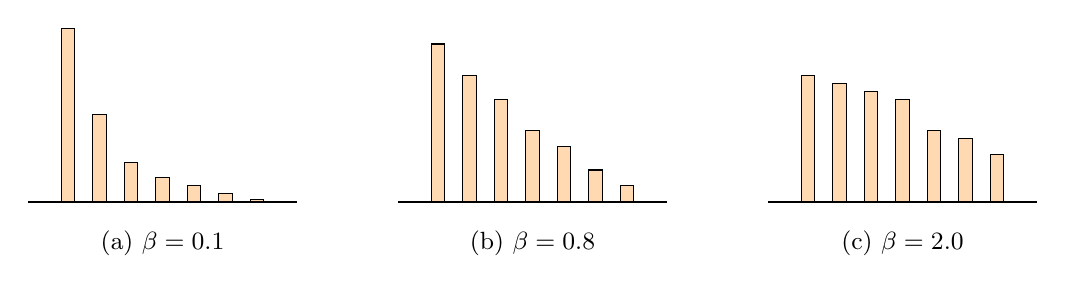
\begin{tikzpicture}
	
\def\ssep{0.4cm}
\def\wbias{0.6cm}
\def\sshift{1.85in}

\tikzstyle{pnode} = [minimum width=0.5em,inner sep=0pt,draw,rounded corners=0pt,fill=orange!30]

\begin{scope}[xshift=0em]

\node [anchor=south,pnode,minimum height=2.2cm] (p1) at (0,0) {};
\node [anchor=south,pnode,minimum height=1.1cm] (p2) at ([xshift=\ssep]p1.south) {};
\node [anchor=south,pnode,minimum height=0.5cm] (p3) at ([xshift=\ssep]p2.south) {};
\node [anchor=south,pnode,minimum height=0.3cm] (p4) at ([xshift=\ssep]p3.south) {};
\node [anchor=south,pnode,minimum height=0.2cm] (p5) at ([xshift=\ssep]p4.south) {};
\node [anchor=south,pnode,minimum height=0.1cm] (p6) at ([xshift=\ssep]p5.south) {};
\node [anchor=south,pnode,minimum height=0.03cm] (p7) at ([xshift=\ssep]p6.south) {};

\draw [-] ([xshift=-\wbias]p1.south east) -- ([xshift=\wbias]p7.south west);

\node [anchor=center] (label) at ([xshift=0,yshift=-\ssep*1.3]p4.south) {\small (a) $\beta=0.1$};

\end{scope}

\begin{scope}[xshift=\sshift]

\node [anchor=south,pnode,minimum height=2.0cm] (p1) at (0,0) {};
\node [anchor=south,pnode,minimum height=1.6cm] (p2) at ([xshift=\ssep]p1.south) {};
\node [anchor=south,pnode,minimum height=1.3cm] (p3) at ([xshift=\ssep]p2.south) {};
\node [anchor=south,pnode,minimum height=0.9cm] (p4) at ([xshift=\ssep]p3.south) {};
\node [anchor=south,pnode,minimum height=0.7cm] (p5) at ([xshift=\ssep]p4.south) {};
\node [anchor=south,pnode,minimum height=0.4cm] (p6) at ([xshift=\ssep]p5.south) {};
\node [anchor=south,pnode,minimum height=0.2cm] (p7) at ([xshift=\ssep]p6.south) {};

\draw [-] ([xshift=-\wbias]p1.south east) -- ([xshift=\wbias]p7.south west);

\node [anchor=center] (label) at ([xshift=0,yshift=-\ssep*1.3]p4.south) {\small (b) $\beta=0.8$};

\end{scope}

\begin{scope}[xshift=\sshift*2]

\node [anchor=south,pnode,minimum height=1.6cm] (p1) at (0,0) {};
\node [anchor=south,pnode,minimum height=1.5cm] (p2) at ([xshift=\ssep]p1.south) {};
\node [anchor=south,pnode,minimum height=1.4cm] (p3) at ([xshift=\ssep]p2.south) {};
\node [anchor=south,pnode,minimum height=1.3cm] (p4) at ([xshift=\ssep]p3.south) {};
\node [anchor=south,pnode,minimum height=0.9cm] (p5) at ([xshift=\ssep]p4.south) {};
\node [anchor=south,pnode,minimum height=0.8cm] (p6) at ([xshift=\ssep]p5.south) {};
\node [anchor=south,pnode,minimum height=0.6cm] (p7) at ([xshift=\ssep]p6.south) {};

\draw [-] ([xshift=-\wbias]p1.south east) -- ([xshift=\wbias]p7.south west);

\node [anchor=center] (label) at ([xshift=0,yshift=-\ssep*1.3]p4.south) {\small (c) $\beta=2.0$};

\end{scope}

\end{tikzpicture}
\end{center}

\vspace{-0.5cm} \caption{温度参数 $\beta$ 取不同值时，Softmax 函数所生成分布的直方图估计。}
\label{fig:llm-softmax-with-temperature}
\end{figure}


\subsubsection{带惩罚项的解码}

文本生成中改进解码方法的一种常见做法，是修改搜索目标。例如，可将最大后验（MAP）解码替换为最小贝叶斯风险（MBR）解码~\cite{kumar-etal:2004minimum}，使关注点从选择概率最高的单个输出，转向选择在可能输出分布上的期望风险最小的输出。这里探讨在解码中引入惩罚项的方法。这类方法简单而有效，能使解码更可控。

回顾式（\ref{eq:llm-general-decoding-objective}），解码的目标是最大化输出序列的似然。加入惩罚项后，目标函数被扩展，以纳入惩罚生成文本中某些行为的额外因素。新目标的一般形式为：
\begin{eqnarray}
\hat{\mathbf{y}} & = & \argmax_{\mathbf{y} \in \mathcal{Y}} \big[ \log \Pr(\mathbf{y}|\mathbf{x}) - \lambda \cdot \mathrm{Penalty}(\mathbf{x},\mathbf{y}) \big], \label{eq:llm-decoding-objective-with-penalty}
\end{eqnarray}

\noindent 其中，$\mathrm{Penalty}(\mathbf{x},\mathbf{y})$ 是一个函数，用于量化在给定输入 $\mathbf{x}$ 时，生成序列 $\mathbf{y}$ 违反特定约束或表现出不期望行为的程度。$\mathrm{Penalty}(\cdot)$ 的设计十分灵活，因此可融入多种约束或先验知识。下面介绍几类常见的惩罚函数。

\begin{itemize}
\item \vspace{0.5em} \textbf{重复惩罚}。重复惩罚用于抑制模型生成重复或冗余文本。惩罚函数可统计生成序列中词元或短语的重复频次，并施加与其出现次数成比例的惩罚。
\item \vspace{0.3em} \textbf{长度惩罚}。长度惩罚用于确保生成序列符合期望长度。例如，在文本摘要任务中，惩罚函数可惩罚过短或过长的输出。
\item \vspace{0.3em} \textbf{多样性惩罚}。多样性惩罚用于促进生成文本的变化。例如，在束搜索中，可度量已生成假设之间的相似度，并鼓励模型探索不同假设。
\item \vspace{0.3em} \textbf{基于约束的惩罚}。基于约束的惩罚用于落实与生成文本内容或风格相关的特定约束。例如，在机器翻译中，惩罚函数可惩罚偏离期望语气或术语的输出。
\end{itemize}
\vspace{0.5em}

通常，可将 $\mathrm{Penalty}(\mathbf{x},\mathbf{y})$ 视为一个函数，为给定输入序列 $\mathbf{x}$ 时生成的序列 $\mathbf{y}$ 指定代价。也可将其定义为评价大语言模型生成 $\mathbf{y}$ 时隐状态的函数。例如，\citet{su-etal:2022contrastive} 设计了一个惩罚项，计算预测词元的表示与先前生成词元的表示之间的最大距离。由此，搜索目标会惩罚包含大量重复等退化输出。

式（\ref{eq:llm-decoding-objective-with-penalty}）所描述的方法具有通用性，可方便地用于不同搜索算法。例如，在贪心搜索中，每个解码步骤可保留使 $\log \Pr(\mathbf{y}|\mathbf{x}) - \lambda \cdot \mathrm{Penalty}(\mathbf{x},\mathbf{y})$ 最大的单个序列；在基于采样的搜索中，可依据 $\log \Pr(\mathbf{y}|\mathbf{x}) - \lambda \cdot \mathrm{Penalty}(\mathbf{x},\mathbf{y})$ 对序列排序，选择排名靠前者构成候选池。

\subsubsection{推测解码}

\mindex{推测解码}源自\mindex{推测执行}的概念：系统对未来操作作出有依据的猜测，并提前执行。如果猜测正确，便可立即使用已有结果，从而加速处理。在大语言模型推理中，假设有两个模型：一个较小且较快的模型，称为草稿模型；另一个完整且能力更强的模型，称为验证模型。这两个模型代表大语言模型推理的两个极端：草稿模型效率高，但准确率较低；验证模型通常才是我们真正希望运行的模型，但速度很慢。给定前缀后，先用草稿模型推测性地预测接下来可能出现的一段词元序列。这是标准的自回归解码过程，但由于草稿模型效率很高，实际执行仍然较快。随后，验证模型并行评价这些推测词元，检查它们是否能被验证模型接受。注意，由于可以同时处理这些词元，验证只需一步即可对所有词元并行完成，无需逐个词元执行。若推测词元正确，就接受它们，并继续处理下一组词元；若不正确，则丢弃错误推测，再由验证模型生成新词元。

更具体地看，\citet{leviathan-etal:2023fast} 提出的推测解码方法使用一个小语言模型作为草稿模型，记为 $\Pr_q(y_i|\mathbf{x},\mathbf{y}_{<i})$；验证模型则是完整的大语言模型，记为 $\Pr_p(y_i|\mathbf{x},\mathbf{y}_{<i})$。其目标是给定前缀后，先使用草稿模型以自回归方式预测至多 $\tau$ 个词元，再由验证模型在推测预测被拒绝的位置生成最后一个词元。图 \ref{fig:speculative-decoding-one-step} 展示了这一解码过程中的一步。为简化说明，这里描述推测解码的贪心版本。

\begin{figure}[!t]
\centering
% !Mode:: "TeX:UTF-8"
% !TEX encoding = UTF-8 Unicode

\begin{center}
\begin{tikzpicture}
	
\def\ssep{1.2cm}

\tikzstyle{lnode} = [minimum width=3.0cm,minimum height=0.6cm,inner sep=2pt,draw,fill=white,rounded corners=0pt]
\tikzstyle{snode} = [minimum width=0.27cm,minimum height=0.18cm,inner sep=2pt,draw,fill=white]

% predictions made by the draft model
\begin{scope}

\node [lnode,anchor=west] (context) at (0,0) {\small{上下文（$\mathbf{x}, \mathbf{y}_{<i}$）}};

\node [anchor=center] (y1) at ([xshift=1.5*\ssep]context.east) {\color{blue} \small{$\hat{y}_{i+1}$}};
\node [anchor=center] (y2) at ([xshift=\ssep]y1.center) {\color{blue} \small{$\hat{y}_{i+2}$}};
\node [anchor=center] (y3) at ([xshift=\ssep]y2.center) {\color{blue} \small{$\hat{y}_{i+3}$}};
\node [anchor=center] (y4) at ([xshift=\ssep]y3.center) {\color{blue} \small{$\hat{y}_{i+4}$}};
\node [anchor=center] (y5) at ([xshift=\ssep]y4.center) {\color{blue} \small{$\hat{y}_{i+5}$}};

\draw [->,double] ([xshift=3pt]context.east) -- ([xshift=-4pt]y1.west);

\draw [-] ([yshift=-0.3cm]y1.west) -- ([yshift=-0.3cm]y5.east);

\node [anchor=north,minimum width=5.7cm,minimum height=0.7cm,draw,thick] (draftmodel) at ([yshift=-0.5cm]y3.south) {\small{草稿模型 $\mathrm{Pr}_q(\cdot)$}};
\draw [->,thick] ([yshift=2pt]draftmodel.north) -- ([yshift=0.4cm]draftmodel.north) node [pos=0.5,right,xshift=0.2cm] (predictlable) {\scriptsize{预测}};

\node [anchor=north] (caption) at ([yshift=-0.3cm,xshift=1cm]draftmodel.south west) {\small{(a) 给定上下文，用草稿模型预测后续 $\tau$ 个词元（$\tau = 5$）}};

\end{scope}

% evaluation by the evaluation model
\begin{scope}[yshift=-5cm]

\node [lnode,anchor=west] (context) at (0,0) {\small{上下文（$\mathbf{x}, \mathbf{y}_{<i}$）}};

\node [anchor=center] (y1) at ([xshift=1.5*\ssep]context.east) {\color{blue} \small{$\hat{y}_{i+1}$}};
\node [anchor=center] (y2) at ([xshift=\ssep]y1.center) {\color{blue} \small{$\hat{y}_{i+2}$}};
\node [anchor=center] (y3) at ([xshift=\ssep]y2.center) {\color{blue} \small{$\hat{y}_{i+3}$}};
\node [anchor=center] (y4) at ([xshift=\ssep]y3.center) {\color{blue} \small{$\hat{y}_{i+4}$}};
\node [anchor=center] (y5) at ([xshift=\ssep]y4.center) {\color{blue} \small{$\hat{y}_{i+5}$}};

\draw [->,double] ([xshift=3pt]context.east) -- ([xshift=-4pt]y1.west);

%\draw [-] ([yshift=-0.3cm]y1.west) -- ([yshift=-0.3cm]y5.east);

\node [anchor=north,minimum width=5.7cm,minimum height=0.7cm,draw=gray!30,thick] (draftmodel) at ([yshift=-0.5cm]y3.south) {\color{gray!30} \small{草稿模型 $\mathrm{Pr}_q(\cdot)$}};
\draw [->,thick,white] ([yshift=2pt]draftmodel.north) -- ([yshift=0.4cm]draftmodel.north);

\node [anchor=south,minimum width=5.7cm,minimum height=0.7cm,draw,thick] (evalmodel) at ([yshift=0.5cm]y3.north) {\small{评估模型 $\mathrm{Pr}_p(\cdot)$}};
\draw [->,thick] ([yshift=-2pt]evalmodel.south) -- ([yshift=-0.4cm]evalmodel.south) node [pos=0.5,right,xshift=0.2cm] (evaluatelable) {\scriptsize{评价}};

\begin{pgfonlayer}{background}
\node [draw,dotted,very thick,inner sep=1pt] [fit = (y1) (y5)] (predictionbox) {};
\end{pgfonlayer}

\node [anchor=north] (caption) at ([yshift=-0.3cm,xshift=1cm]draftmodel.south west) {\small{(b) 使用评估模型评价预测词元}};

\end{scope}

% determining accepted guesses
\begin{scope}[yshift=-10cm]

\node [lnode,anchor=west] (context) at (0,0) {\small{上下文（$\mathbf{x}, \mathbf{y}_{<i}$）}};

\node [anchor=center] (y1) at ([xshift=1.5*\ssep]context.east) {\color{blue} \small{$\hat{y}_{i+1}$}};
\node [anchor=center] (y2) at ([xshift=\ssep]y1.center) {\color{blue} \small{$\hat{y}_{i+2}$}};
\node [anchor=center] (y3) at ([xshift=\ssep]y2.center) {\color{blue} \small{$\hat{y}_{i+3}$}};
\node [anchor=center] (y4) at ([xshift=\ssep]y3.center) {\color{blue} \small{$\hat{y}_{i+4}$}};
\node [anchor=center] (y5) at ([xshift=\ssep]y4.center) {\color{blue} \small{$\hat{y}_{i+5}$}};

\draw [->,double] ([xshift=3pt]context.east) -- ([xshift=-4pt]y1.west);

%\draw [-] ([yshift=-0.3cm]y1.west) -- ([yshift=-0.3cm]y5.east);

\node [anchor=north,minimum width=5.7cm,minimum height=0.7cm,draw=gray!30,thick] (draftmodel) at ([yshift=-0.5cm]y3.south) {\color{gray!30} \small{草稿模型 $\mathrm{Pr}_q(\cdot)$}};
\draw [->,thick,white] ([yshift=2pt]draftmodel.north) -- ([yshift=0.4cm]draftmodel.north);

\node [anchor=south,minimum width=5.7cm,minimum height=0.7cm,draw=gray!30,thick] (evalmodel) at ([yshift=0.5cm]y3.north) {\color{gray!30} \small{评估模型 $\mathrm{Pr}_p(\cdot)$}};
\draw [->,thick,white] ([yshift=-2pt]evalmodel.south) -- ([yshift=-0.4cm]evalmodel.south);

\begin{pgfonlayer}{background}
\node [draw=blue,dotted,very thick,inner sep=1pt] [fit = (y1) (y3)] (predictionbox) {};
\node [draw=red,dotted,very thick,inner sep=1pt] [fit = (y4) (y5)] (predictionbox2) {};
\end{pgfonlayer}

\node [anchor=south] (acceptedlabel) at (predictionbox.north) {\color{blue} \scriptsize{接受}};
\node [anchor=south] (rejectedlabel) at (predictionbox2.north) {\color{red} \scriptsize{拒绝}};
\draw [-,red] ([yshift=-2pt,xshift=3pt]predictionbox2.north west) -- ([yshift=2pt,xshift=-3pt]predictionbox2.south east);
\draw [-,red] ([yshift=-2pt,xshift=-3pt]predictionbox2.north east) -- ([yshift=2pt,xshift=3pt]predictionbox2.south west);

\node [anchor=north] (caption) at ([yshift=-0.3cm,xshift=1cm]draftmodel.south west) {\small{(c) 确定接受的词元数}};

\end{scope}

% predicting a new token
\begin{scope}[yshift=-15cm]

\node [lnode,anchor=west] (context) at (0,0) {\small{上下文（$\mathbf{x}, \mathbf{y}_{<i}$）}};

\node [anchor=center] (y1) at ([xshift=1.5*\ssep]context.east) {\color{blue} \small{$\hat{y}_{i+1}$}};
\node [anchor=center] (y2) at ([xshift=\ssep]y1.center) {\color{blue} \small{$\hat{y}_{i+2}$}};
\node [anchor=center] (y3) at ([xshift=\ssep]y2.center) {\color{blue} \small{$\hat{y}_{i+3}$}};
\node [anchor=center,fill=gray!30] (y4) at ([xshift=\ssep]y3.center) {\color{black} \small{$\bar{y}_{i+4}$}};

\draw [->,double] ([xshift=3pt]context.east) -- ([xshift=-4pt]y1.west);

%\draw [-] ([yshift=-0.3cm]y1.west) -- ([yshift=-0.3cm]y5.east);
\draw [<-,thick] ([yshift=2pt]y4.north) -- ([yshift=0.45cm]y4.north);

\node [anchor=north,minimum width=5.7cm,minimum height=0.7cm,draw=gray!30,thick] (draftmodel) at ([yshift=-0.5cm]y3.south) {\color{gray!30} \small{草稿模型 $\mathrm{Pr}_q(\cdot)$}};
\draw [->,thick,white] ([yshift=2pt]draftmodel.north) -- ([yshift=0.4cm]draftmodel.north);

\node [anchor=south,minimum width=5.7cm,minimum height=0.7cm,draw,thick] (evalmodel) at ([yshift=0.5cm]y3.north) {\small{评估模型 $\mathrm{Pr}_p(\cdot)$}};
\draw [->,thick,white] ([yshift=-2pt]evalmodel.south) -- ([yshift=-0.4cm]evalmodel.south);

\node [anchor=north] (caption) at ([yshift=-0.3cm,xshift=1cm]draftmodel.south west) {\small{(d) 使用评估模型在已接受词元之后预测一个新词元}};

\end{scope}

\end{tikzpicture}
\end{center}

\vspace{-0.5cm} \caption{推测解码的一个步骤。目标是使用草稿模型预测尽可能多的后续词元。该过程包含四个子步骤：首先，给定上下文，用草稿模型预测后续 $\tau$ 个词元；然后，用验证模型并行评价这些预测；接着，确定可接受的预测词元的最大数量；最后，用评估模型在这些已接受词元之后预测一个新词元。}
\label{fig:speculative-decoding-one-step}
\end{figure}

推测解码算法可概括如下。

\begin{itemize}
\item \vspace{0.5em} 给定前缀 $[\mathbf{x},\mathbf{y}_{\le i}]$，使用草稿模型连续预测后续 $\tau$ 个词元，记为 $\{\hat{y}_{i+1},\cdots,\hat{y}_{i+\tau}\}$。这是一个逐词元生成过程，形式为：
    \begin{eqnarray}
    \hat{y}_{i+t} & = & \argmax_{y_{i+t}} \mathrm{Pr}_q(y_{i+t}|\mathbf{x},\mathbf{y}_{\le i},\hat{y}_{i+1}\cdots\hat{y}_{i+t-1}).
    \end{eqnarray}
\item \vspace{0.3em} 使用验证模型评价 $\{\hat{y}_{i+1},\cdots,\hat{y}_{i+\tau}\}$，即计算\\ $\{\mathrm{Pr}_p(\hat{y}_{i+1}|\mathbf{x},\mathbf{y}_{\le i})$ $,\cdots,\mathrm{Pr}_p(\hat{y}_{i+\tau}|\mathbf{x},\mathbf{y}_{\le i},\hat{y}_{i+1}\cdots\hat{y}_{i+\tau-1})\}$。注意，这些概率可以并行计算，因此该验证步骤是高效的。
\item \vspace{0.3em} 确定可接受的推测词元的最大数量。为使记号简洁，将 $\mathrm{Pr}_q(\hat{y}_{i+t}|\mathbf{x},\mathbf{y}_{\le i},\hat{y}_{i+1}\cdots\hat{y}_{i+t-1})$ 和 $\mathrm{Pr}_p(\hat{y}_{i+t}|\mathbf{x},\mathbf{y}_{\le i},\hat{y}_{i+1}\cdots\hat{y}_{i+t-1})$ 分别简记为 $q(\hat{y}_{i+t})$ 与 $p(\hat{y}_{i+t})$。接受规则定义如下：若 $q(\hat{y}_{i+t}) \le p(\hat{y}_{i+t})$，则接受该推测；若 $q(\hat{y}_{i+t}) > p(\hat{y}_{i+t})$，则以概率 $1-\frac{p(\hat{y}_{i+t})}{q(\hat{y}_{i+t})}$ 拒绝该推测。从 $\hat{y}_{i+1}$ 开始，可接受的连续推测词元的最大数量定义为：
    \begin{eqnarray}
    n_a & = & \min \left\{t-1 | 1 \le t \le \tau, r_t > \frac{p(\hat{y}_{i+t})}{q(\hat{y}_{i+t})} \right\},
    \end{eqnarray}
    \noindent 其中，$r_t$ 是从均匀分布 $U(0,1)$ 中抽取的变量。若所有推测词元均被接受，则令 $n_a=\tau$。
\item 给定 $n_a$，保留推测词元 $\{\hat{y}_{i+1},\cdots,\hat{y}_{i+n_a}\}$，再由验证模型在 $i+n_a+1$ 处作出新的预测：
    \begin{eqnarray}
    \bar{y}_{i+n_a+1} & = & \argmax_{y_{i+n_a+1}} \mathrm{Pr}_p(y_{i+n_a+1}|\mathbf{x},\mathbf{y}_{\le i},\hat{y}_{i+1}\cdots\hat{y}_{i+n_a}).
    \end{eqnarray}
\item 上面描述了推测解码的一个步骤。所得序列（包含上下文与预测词元）如下图所示：
\begin{center}
% !Mode:: "TeX:UTF-8"
% !TEX encoding = UTF-8 Unicode

\begin{center}
\begin{tikzpicture}
	
\def\ssep{0.8cm}
\def\nodew{10cm}

\tikzstyle{lnode} = [minimum width=3cm,minimum height=1.0cm,inner sep=2pt,draw,thick,fill=white,rounded corners=1pt]
\tikzstyle{snode} = [circle,minimum size=0.2cm,inner sep=0,draw=white,line width=0.02cm,fill=black]

\begin{scope}

\node[anchor=west] (s1) at (0,0) {$[\mathbf{x},\ \ \mathbf{y}_{<i}]$};
\node[anchor=west] (s2) at ([xshift=0.1cm]s1.east) {$\hat{y}_{i+1} ... \hat{y}_{i+n_a}$};
\node[anchor=west] (s3) at ([xshift=0.1cm,yshift=-1pt]s2.east) {$\bar{y}_{i+n_a+1}$};

\draw [decoration={brace,amplitude=4pt},decorate] ([yshift=-0.0cm,xshift=-2pt]s1.south east) -- ([yshift=-0.0cm,xshift=2pt]s1.south west) node [pos=0.5,below,yshift=-0.1cm] {\scriptsize{上下文}};
\draw [decoration={brace,amplitude=4pt},decorate] ([yshift=-0.0cm,xshift=-2pt]s2.south east) -- ([yshift=-0.0cm,xshift=2pt]s2.south west) node [pos=0.5,below,yshift=-0.1cm,align=left] {\scriptsize{$n_a$ 个词元}\\[-0.15cm] \scriptsize{由以下模型预测：}\\[-0.15cm] \scriptsize{草稿模型}};
\draw [decoration={brace,amplitude=4pt},decorate] ([yshift=-0.0cm,xshift=-3pt]s3.south east) -- ([yshift=-0.0cm,xshift=3pt]s3.south west) node [pos=0.5,below,yshift=-0.1cm,xshift=0.5cm,align=left] {\scriptsize{一个词元}\\[-0.15cm] \scriptsize{由以下模型预测：}\\[-0.15cm] \scriptsize{验证模型}};

\end{scope}

\end{tikzpicture}
\end{center}

\end{center}
    完成该步骤后，将预测词元 $\{\hat{y}_{i+1},\cdots,\hat{y}_{i+n_a},\bar{y}_{i+n_a+1} \}$ 加入上下文，并重复上述过程。
\end{itemize}
\vspace{0.5em}

实践中，通常希望使用较小的草稿模型，使预测 $\{\hat{y}_{i+1},\cdots,\hat{y}_{i+n_a}\}$ 的计算开销更低。不过，草稿模型过小会降低准确率，导致 $n_a$ 较小。因此，需要审慎选择草稿模型，在计算效率与准确率之间作出权衡。

\subsubsection{停止条件}

停止条件是大语言模型推理的重要组成部分，通常由规定模型何时停止解码文本的规则或条件构成。多数大语言模型在训练中会学习生成序列结束词元（例如 $\langle \mathrm{EOS} \rangle$ 或 $\langle /s \rangle$），以标记生成文本的结束。因此，最简单的策略是在生成该词元时停止。束搜索同时探索多个假设，可持续进行，直到生成给定数量的完整序列。

在实际应用中，通常并不希望生成过长的序列，因此需要降低解码开销，避免不必要的冗长。一种常用停止条件是输出的最大长度：模型生成预定数量的词元后即停止。也可依据实际计算开销停止解码，例如计算资源或时间限制。以聊天机器人等实时应用为例，为保证响应速度，可能需要在达到某个时间上限后停止解码。

另一种方法是根据大语言模型的行为设计停止条件。例如，当预测下一词元的概率低于某个阈值时停止解码。除基于概率的停止条件外，还可实现重复检测模块：当模型重复生成词元或短语超过预设上限时，触发停止。这有助于避免冗余或不连贯的输出。

\subsection{大语言模型推理的评价指标}

评价大语言模型推理系统的性能，需要使用多种指标，考察模型在质量、稳健性、可用性与效率等方面达到预期标准的程度。与多数自然语言处理系统一样，可使用困惑度、F1 分数等标准指标评价大语言模型。也可测试它们处理歧义输入或困难输入的能力，包括对抗样本、扰动输入及分布外数据，以考察稳健性。此外，可从流畅性、连贯性、相关性与多样性等方面，度量生成输出符合用户预期的程度，以评价可用性。人工评价者可为文本的自然程度评分，或判断回复是否符合上下文、逻辑是否一致。还可纳入伦理与公平性指标，确保大语言模型避免延续偏见或生成有害内容。

以上评价指标主要关注输出质量。考虑到大语言模型部署和服务的高昂开销，效率指标对实践者同样十分重要。下面列出一些常用的效率指标~\cite{nvidia-nim-llm-benchmarking}：

\begin{itemize}
\item \vspace{0.5em} \textbf{请求时延}。从向大语言模型发送请求，到收到完整回复所需的总时间，包括数据传输、模型处理以及将输出返回用户的时间。
\item \vspace{0.3em} \textbf{吞吐量}。系统单位时间内能够处理的请求数或生成的词元数。吞吐量通常以每秒请求数（RPS）或每秒词元数（TPS）报告。
\item \vspace{0.3em} \textbf{首词元时延}（TTFT）。从发送请求到生成回复中第一个词元之间的时间。若数据传输耗时较少，TTFT 主要由预填充阶段的耗时与生成第一个词元的耗时组成。
\item \vspace{0.3em} \textbf{词元间时延}（ITL）。生成第一个词元之后，每个后续词元所需的生成时间，反映解码过程的效率。
\item \vspace{0.3em} \textbf{资源利用率}。衡量模型推理过程中的计算资源使用情况（例如 CPU 和 GPU 利用率）以及内存消耗。
\end{itemize}
\vspace{0.5em}

除上述指标外，能效与成本效益也是大规模部署大语言模型时的实际考虑因素。能效衡量模型推理过程中的电力消耗；成本效益则评价部署与维护模型相关的总支出。

总体而言，评价指标的选择取决于具体任务与应用。质量指标对于评价大语言模型必不可少，效率指标对于模型在实际应用中的有效部署也同样关键。完整的评价框架应兼顾这两类指标，以准确衡量大语言模型的性能与实用性。

%----------------------------------------------------------------------------------------
% NEW SECTION
%----------------------------------------------------------------------------------------

\section{高效推理技术}

在实际应用中，通常希望系统尽可能高效。对于大语言模型推理，这通常涉及两类改进：降低内存需求与加速推理。例如，可修改 Transformer 架构，避免在处理极长输入序列时出现内存需求激增；也可在保留语义信息的同时压缩输入序列，以降低计算开销。此外，还可使用量化与剪枝等技术，进一步优化内存使用与推理速度。

高效推理是一个涉及面很广的主题，与架构设计、模型压缩等多个大语言模型研究方向交叉。前面各章已介绍其中大多数主题。例如，第 \ChapterLLM 章讨论了长上下文大语言模型，第 \ChapterLLMPrompting 章讨论了用于缩短提示长度的提示压缩方法。本节聚焦大语言模型部署与服务中常用的技术。

\subsection{前缀缓存}

在实际应用中，缓存常见请求及其对应回复是常见做法。当新请求命中缓存时，系统可直接从缓存中取出回复，无需重新计算。一种直接的实现方式是使用键值数据存储（例如哈希表），建立输入序列到大语言模型所生成输出序列的映射。最简单的情形下，可收集常见查询，用大语言模型生成回复，再将这些查询—回复对存入数据存储中。这样便建立了基本的序列级缓存机制：当输入序列与缓存查询完全匹配时，系统即可跳过大语言模型计算。

这一缓存机制可自然扩展为缓存前缀及其对应的 KV 缓存状态。给定数据集 $\mathcal{D}$ 中的输入序列 $\mathbf{x}$，按标准预填充阶段处理它，即可得到一系列前缀及其对应的 KV 缓存状态：
\begin{eqnarray}
x_0\ (\text{即 } \mathbf{x}_{<1}) & \Rightarrow & \mathrm{cache}_{<1} \nonumber \\
x_0 x_1\ (\text{即 } \mathbf{x}_{<2}) & \Rightarrow & \mathrm{cache}_{<2} \nonumber \\
& \cdots & \nonumber \\
x_0 x_1 \cdots x_{m-1}\ (\text{即 } \mathbf{x}_{<m}) & \Rightarrow & \mathrm{cache}_{<m} \nonumber
\end{eqnarray}

\noindent 其中，$\mathrm{cache}_{<i}$ 表示前缀 $\mathbf{x}_{<i}$ 的 KV 缓存（亦见式（\ref{eq:prefilling-kv-cache}））。所有这些映射均可存入前缀缓存，以便高效复用。

当新序列与 $\mathcal{D}$ 中先前处理过的某个序列共享前缀时，可直接加载缓存的对应 KV 状态，无需重新计算。具体而言，若新输入 $\mathbf{x}'$ 与已有序列共享前缀 $\mathbf{x}_{<k}$（即存在 $k \le m$，使 $\mathbf{x}'_{<k} = \mathbf{x}_{<k}$），就可用 $\mathrm{cache}_{<k}$ 初始化 KV 缓存，仅计算剩余词元 $\mathbf{x}'_{\ge k}$ 的 KV 状态。

与通常做法一样，可维护一个键值数据存储，将常见前缀映射到预先计算的 KV 缓存。查询时，可使用前缀词元的哈希值，以常数时间访问缓存状态。需要注意内存管理，因为对于大型数据集，存储所有可能前缀未必可行。实际系统通常采用最近最少使用（LRU）缓存方法或其他策略，在节省计算与内存限制之间取得平衡。

\subsection{批处理}

大语言模型推理中的批处理，是指将多个输入序列组成一组（称为一个批次），同时处理，而非逐个处理。现代 GPU 擅长并行计算，批处理可使它们在一次前向传播中计算多个序列，充分占用硬件。因此，在大规模提供大语言模型服务时，批处理对于提高计算效率、最大化硬件利用率十分重要\footnote{简单的评价可参见 \url{https://docs.nvidia.com/deeplearning/performance/dl-performance-gpu-background/index.html\#understand-perf}。}。

为说明批处理的思想，图 \ref{fig:basic-llm-batching-methods}（a—b）分别给出批大小为 1 和 4 的简单示例。批大小为 1 时（即不进行批处理），GPU 每次只处理一个输入序列。因此，处理是顺序进行的：下一个序列必须等待当前计算完成。相比之下，批大小为 4 时，GPU 可在一次前向传播中同时处理四个序列。由于输入序列长度不同，需要用填充技术统一长度。这里采用左侧填充，即在较短序列的开头添加占位词元，使同一批次中所有序列在预填充时具有相同长度。解码时，同时为这些序列生成词元，直到该批次所有序列均完成解码。

\begin{figure}[!t]
\centering
% !Mode:: "TeX:UTF-8"
% !TEX encoding = UTF-8 Unicode

\begin{center}
\begin{tikzpicture}
	
\def\ssep{0.12cm}

\tikzstyle{lnode} = [minimum width=3.0cm,minimum height=0.6cm,inner sep=2pt,draw,fill=white,rounded corners=0pt]
\tikzstyle{snode} = [minimum width=0.33cm,minimum height=0.33cm,inner sep=0pt,draw,fill=white]

% inference (batch size = 1)
\begin{scope}

\node [snode,anchor=west,fill=red!30] (x00) at (0,0) {};
\node [snode,anchor=east,fill=red!30] (x01) at ([xshift=-\ssep]x00.west) {};
\node [snode,anchor=east,fill=red!30] (x02) at ([xshift=-\ssep]x01.west) {};
\node [snode,anchor=east,fill=red!30] (x03) at ([xshift=-\ssep]x02.west) {};
\node [snode,anchor=east,fill=red!30] (x04) at ([xshift=-\ssep]x03.west) {};

\node [snode,anchor=west,fill=blue!30] (y01) at ([xshift=2*\ssep]x00.east) {};
\node [snode,anchor=west,fill=blue!30] (y02) at ([xshift=\ssep]y01.east) {};
\node [snode,anchor=west,fill=blue!30] (y03) at ([xshift=\ssep]y02.east) {};
\node [snode,anchor=west,fill=blue!30] (y04) at ([xshift=\ssep]y03.east) {};

\draw [decoration={brace,amplitude=4pt},decorate] ([yshift=0.1cm,xshift=0.0cm]x04.north west) -- ([yshift=0.1cm,xshift=0.0cm]x00.north east) node [above,pos=0.5,yshift=0.1cm] {\scriptsize{预填充}};
\draw [decoration={brace,amplitude=4pt},decorate] ([yshift=0.1cm,xshift=0.0cm]y01.north west) -- ([yshift=0.1cm,xshift=0.0cm]y04.north east) node [above,pos=0.5,yshift=0.1cm] {\scriptsize{解码}};

\node [anchor=north] (caption) at ([yshift=-2cm]x00.south east) {\footnotesize{(a) 批大小 $= 1$}};

\end{scope}

% inference (batch size = 4)
\begin{scope}[xshift=7.5cm]

\node [snode,anchor=west,fill=red!30] (x00) at (0,0) {\scriptsize{1}};
\node [snode,anchor=east,fill=red!30] (x01) at ([xshift=-\ssep]x00.west) {\scriptsize{1}};
\node [snode,anchor=east,fill=red!30] (x02) at ([xshift=-\ssep]x01.west) {\scriptsize{1}};
\node [snode,anchor=east,fill=red!30] (x03) at ([xshift=-\ssep]x02.west) {\scriptsize{1}};
\node [snode,anchor=east,fill=red!30] (x04) at ([xshift=-\ssep]x03.west) {\scriptsize{1}};
\node [snode,anchor=east,fill=ugreen!30] (x05) at ([xshift=-\ssep]x04.west) {\tiny{填充}};

\node [snode,anchor=west,fill=blue!30] (y01) at ([xshift=2*\ssep]x00.east) {\scriptsize{1}};
\node [snode,anchor=west,fill=blue!30] (y02) at ([xshift=\ssep]y01.east) {\scriptsize{1}};
\node [snode,anchor=west,fill=blue!30] (y03) at ([xshift=\ssep]y02.east) {\scriptsize{1}};
\node [snode,anchor=west,fill=blue!30] (y04) at ([xshift=\ssep]y03.east) {\scriptsize{1}};
\node [snode,anchor=west,fill=gray!30] (y05) at ([xshift=\ssep]y04.east) {};
\node [snode,anchor=west,fill=gray!30] (y06) at ([xshift=\ssep]y05.east) {};

\node [snode,anchor=north,fill=red!30] (x10) at ([yshift=-\ssep]x00.south) {\scriptsize{2}};
\node [snode,anchor=east,fill=red!30] (x11) at ([xshift=-\ssep]x10.west) {\scriptsize{2}};
\node [snode,anchor=east,fill=red!30] (x12) at ([xshift=-\ssep]x11.west) {\scriptsize{2}};
\node [snode,anchor=east,fill=red!30] (x13) at ([xshift=-\ssep]x12.west) {\scriptsize{2}};
\node [snode,anchor=east,fill=ugreen!30] (x14) at ([xshift=-\ssep]x13.west) {\tiny{填充}};
\node [snode,anchor=east,fill=ugreen!30] (x15) at ([xshift=-\ssep]x14.west) {\tiny{填充}};

\node [snode,anchor=west,fill=blue!30] (y11) at ([xshift=2*\ssep]x10.east) {\scriptsize{2}};
\node [snode,anchor=west,fill=blue!30] (y12) at ([xshift=\ssep]y11.east) {\scriptsize{2}};
\node [snode,anchor=west,fill=blue!30] (y13) at ([xshift=\ssep]y12.east) {\scriptsize{2}};
\node [snode,anchor=west,fill=gray!30] (y14) at ([xshift=\ssep]y13.east) {};
\node [snode,anchor=west,fill=gray!30] (y15) at ([xshift=\ssep]y14.east) {};
\node [snode,anchor=west,fill=gray!30] (y16) at ([xshift=\ssep]y15.east) {};

\node [snode,anchor=north,fill=red!30] (x20) at ([yshift=-\ssep]x10.south) {\scriptsize{3}};
\node [snode,anchor=east,fill=red!30] (x21) at ([xshift=-\ssep]x20.west) {\scriptsize{3}};
\node [snode,anchor=east,fill=red!30] (x22) at ([xshift=-\ssep]x21.west) {\scriptsize{3}};
\node [snode,anchor=east,fill=ugreen!30] (x23) at ([xshift=-\ssep]x22.west) {\tiny{填充}};
\node [snode,anchor=east,fill=ugreen!30] (x24) at ([xshift=-\ssep]x23.west) {\tiny{填充}};
\node [snode,anchor=east,fill=ugreen!30] (x25) at ([xshift=-\ssep]x24.west) {\tiny{填充}};

\node [snode,anchor=west,fill=blue!30] (y21) at ([xshift=2*\ssep]x20.east) {\scriptsize{3}};
\node [snode,anchor=west,fill=blue!30] (y22) at ([xshift=\ssep]y21.east) {\scriptsize{3}};
\node [snode,anchor=west,fill=gray!30] (y23) at ([xshift=\ssep]y22.east) {};
\node [snode,anchor=west,fill=gray!30] (y24) at ([xshift=\ssep]y23.east) {};
\node [snode,anchor=west,fill=gray!30] (y25) at ([xshift=\ssep]y24.east) {};
\node [snode,anchor=west,fill=gray!30] (y26) at ([xshift=\ssep]y25.east) {};

\node [snode,anchor=north,fill=red!30] (x30) at ([yshift=-\ssep]x20.south) {\scriptsize{4}};
\node [snode,anchor=east,fill=red!30] (x31) at ([xshift=-\ssep]x30.west) {\scriptsize{4}};
\node [snode,anchor=east,fill=red!30] (x32) at ([xshift=-\ssep]x31.west) {\scriptsize{4}};
\node [snode,anchor=east,fill=red!30] (x33) at ([xshift=-\ssep]x32.west) {\scriptsize{4}};
\node [snode,anchor=east,fill=red!30] (x34) at ([xshift=-\ssep]x33.west) {\scriptsize{4}};
\node [snode,anchor=east,fill=red!30] (x35) at ([xshift=-\ssep]x34.west) {\scriptsize{4}};

\node [snode,anchor=west,fill=blue!30] (y31) at ([xshift=2*\ssep]x30.east) {\scriptsize{4}};
\node [snode,anchor=west,fill=blue!30] (y32) at ([xshift=\ssep]y31.east) {\scriptsize{4}};
\node [snode,anchor=west,fill=blue!30] (y33) at ([xshift=\ssep]y32.east) {\scriptsize{4}};
\node [snode,anchor=west,fill=blue!30] (y34) at ([xshift=\ssep]y33.east) {\scriptsize{4}};
\node [snode,anchor=west,fill=blue!30] (y35) at ([xshift=\ssep]y34.east) {\scriptsize{4}};
\node [snode,anchor=west,fill=blue!30] (y36) at ([xshift=\ssep]y35.east) {\scriptsize{4}};

\draw [decoration={brace,amplitude=4pt},decorate] ([yshift=0.1cm,xshift=0.0cm]x05.north west) -- ([yshift=0.1cm,xshift=0.0cm]x00.north east) node [above,pos=0.5,yshift=0.1cm] {\scriptsize{预填充}};
\draw [decoration={brace,amplitude=4pt},decorate] ([yshift=0.1cm,xshift=0.0cm]y01.north west) -- ([yshift=0.1cm,xshift=0.0cm]y06.north east) node [above,pos=0.5,yshift=0.1cm] {\scriptsize{解码}};

\node [anchor=north] (caption) at ([yshift=-2cm]x00.south east) {\footnotesize{(b) 批大小 $= 4$}};

\end{scope}

% inference (batch size = 4, sorted by length)
\begin{scope}[yshift=-5.3cm]

\node [snode,anchor=west,fill=red!30] (x00) at (0,0) {\scriptsize{1}};
\node [snode,anchor=east,fill=red!30] (x01) at ([xshift=-\ssep]x00.west) {\scriptsize{1}};
\node [snode,anchor=east,fill=red!30] (x02) at ([xshift=-\ssep]x01.west) {\scriptsize{1}};
\node [snode,anchor=east,fill=red!30] (x03) at ([xshift=-\ssep]x02.west) {\scriptsize{1}};
\node [snode,anchor=east,fill=red!30] (x04) at ([xshift=-\ssep]x03.west) {\scriptsize{1}};
\node [snode,anchor=east,fill=ugreen!30] (x05) at ([xshift=-\ssep]x04.west) {\tiny{填充}};

\node [snode,anchor=west,fill=blue!30] (y01) at ([xshift=2*\ssep]x00.east) {\scriptsize{1}};
\node [snode,anchor=west,fill=blue!30] (y02) at ([xshift=\ssep]y01.east) {\scriptsize{1}};
\node [snode,anchor=west,fill=blue!30] (y03) at ([xshift=\ssep]y02.east) {\scriptsize{1}};
\node [snode,anchor=west,fill=blue!30] (y04) at ([xshift=\ssep]y03.east) {\scriptsize{1}};
\node [snode,anchor=west,fill=blue!30] (y05) at ([xshift=\ssep]y04.east) {\scriptsize{1}};
\node [snode,anchor=west,fill=blue!30] (y06) at ([xshift=\ssep]y05.east) {\scriptsize{1}};

\node [snode,anchor=north,fill=red!30] (x10) at ([yshift=-\ssep]x00.south) {\scriptsize{2}};
\node [snode,anchor=east,fill=red!30] (x11) at ([xshift=-\ssep]x10.west) {\scriptsize{2}};
\node [snode,anchor=east,fill=red!30] (x12) at ([xshift=-\ssep]x11.west) {\scriptsize{2}};
\node [snode,anchor=east,fill=red!30] (x13) at ([xshift=-\ssep]x12.west) {\scriptsize{2}};
\node [snode,anchor=east,fill=red!30] (x14) at ([xshift=-\ssep]x13.west) {\scriptsize{2}};
\node [snode,anchor=east,fill=ugreen!30] (x15) at ([xshift=-\ssep]x14.west) {\tiny{填充}};

\node [snode,anchor=west,fill=blue!30] (y11) at ([xshift=2*\ssep]x10.east) {\scriptsize{2}};
\node [snode,anchor=west,fill=blue!30] (y12) at ([xshift=\ssep]y11.east) {\scriptsize{2}};
\node [snode,anchor=west,fill=blue!30] (y13) at ([xshift=\ssep]y12.east) {\scriptsize{2}};
\node [snode,anchor=west,fill=blue!30] (y14) at ([xshift=\ssep]y13.east) {\scriptsize{2}};
\node [snode,anchor=west,fill=blue!30] (y15) at ([xshift=\ssep]y14.east) {\scriptsize{2}};
\node [snode,anchor=west,fill=gray!30] (y16) at ([xshift=\ssep]y15.east) {};

\node [snode,anchor=north,fill=red!30] (x20) at ([yshift=-\ssep]x10.south) {\scriptsize{3}};
\node [snode,anchor=east,fill=red!30] (x21) at ([xshift=-\ssep]x20.west) {\scriptsize{3}};
\node [snode,anchor=east,fill=red!30] (x22) at ([xshift=-\ssep]x21.west) {\scriptsize{3}};
\node [snode,anchor=east,fill=red!30] (x23) at ([xshift=-\ssep]x22.west) {\scriptsize{3}};
\node [snode,anchor=east,fill=red!30] (x24) at ([xshift=-\ssep]x23.west) {\scriptsize{3}};
\node [snode,anchor=east,fill=red!30] (x25) at ([xshift=-\ssep]x24.west) {\scriptsize{3}};

\node [snode,anchor=west,fill=blue!30] (y21) at ([xshift=2*\ssep]x20.east) {\scriptsize{3}};
\node [snode,anchor=west,fill=blue!30] (y22) at ([xshift=\ssep]y21.east) {\scriptsize{3}};
\node [snode,anchor=west,fill=blue!30] (y23) at ([xshift=\ssep]y22.east) {\scriptsize{3}};
\node [snode,anchor=west,fill=blue!30] (y24) at ([xshift=\ssep]y23.east) {\scriptsize{3}};
\node [snode,anchor=west,fill=blue!30] (y25) at ([xshift=\ssep]y24.east) {\scriptsize{3}};
\node [snode,anchor=west,fill=gray!30] (y26) at ([xshift=\ssep]y25.east) {};

\node [snode,anchor=north,fill=red!30] (x30) at ([yshift=-\ssep]x20.south) {\scriptsize{4}};
\node [snode,anchor=east,fill=red!30] (x31) at ([xshift=-\ssep]x30.west) {\scriptsize{4}};
\node [snode,anchor=east,fill=red!30] (x32) at ([xshift=-\ssep]x31.west) {\scriptsize{4}};
\node [snode,anchor=east,fill=red!30] (x33) at ([xshift=-\ssep]x32.west) {\scriptsize{4}};
\node [snode,anchor=east,fill=red!30] (x34) at ([xshift=-\ssep]x33.west) {\scriptsize{4}};
\node [snode,anchor=east,fill=red!30] (x35) at ([xshift=-\ssep]x34.west) {\scriptsize{4}};

\node [snode,anchor=west,fill=blue!30] (y31) at ([xshift=2*\ssep]x30.east) {\scriptsize{4}};
\node [snode,anchor=west,fill=blue!30] (y32) at ([xshift=\ssep]y31.east) {\scriptsize{4}};
\node [snode,anchor=west,fill=blue!30] (y33) at ([xshift=\ssep]y32.east) {\scriptsize{4}};
\node [snode,anchor=west,fill=blue!30] (y34) at ([xshift=\ssep]y33.east) {\scriptsize{4}};
\node [snode,anchor=west,fill=blue!30] (y35) at ([xshift=\ssep]y34.east) {\scriptsize{4}};
\node [snode,anchor=west,fill=blue!30] (y36) at ([xshift=\ssep]y35.east) {\scriptsize{4}};

\draw [decoration={brace,amplitude=4pt},decorate] ([yshift=0.1cm,xshift=0.0cm]x05.north west) -- ([yshift=0.1cm,xshift=0.0cm]x00.north east) node [above,pos=0.5,yshift=0.1cm] {\scriptsize{预填充}};
\draw [decoration={brace,amplitude=4pt},decorate] ([yshift=0.1cm,xshift=0.0cm]y01.north west) -- ([yshift=0.1cm,xshift=0.0cm]y06.north east) node [above,pos=0.5,yshift=0.1cm] {\scriptsize{解码}};

\node [anchor=north] (caption) at ([yshift=-2.9cm,xshift=0.1cm]x00.south east) {\footnotesize{(c) 批大小 $= 4$（序列长度相近）}};

\end{scope}

% inference (batch size = 4)
\begin{scope}[xshift=7.5cm,yshift=-5.3cm]

\node [snode,anchor=west,fill=red!30] (x00) at (0,0) {\scriptsize{1}};
\node [snode,anchor=east,fill=red!30] (x01) at ([xshift=-\ssep]x00.west) {\scriptsize{1}};
\node [snode,anchor=east,fill=red!30] (x02) at ([xshift=-\ssep]x01.west) {\scriptsize{1}};
\node [snode,anchor=east,fill=red!30] (x03) at ([xshift=-\ssep]x02.west) {\scriptsize{1}};
\node [snode,anchor=east,fill=red!30] (x04) at ([xshift=-\ssep]x03.west) {\scriptsize{1}};
\node [snode,anchor=east,fill=ugreen!30] (x05) at ([xshift=-\ssep]x04.west) {\tiny{填充}};

\node [snode,anchor=west,fill=blue!30] (y01) at ([xshift=2*\ssep]x00.east) {\scriptsize{1}};
\node [snode,anchor=west,fill=blue!30] (y02) at ([xshift=\ssep]y01.east) {\scriptsize{1}};
\node [snode,anchor=west,fill=blue!30] (y03) at ([xshift=\ssep]y02.east) {\scriptsize{1}};
\node [snode,anchor=west,fill=blue!30] (y04) at ([xshift=\ssep]y03.east) {\scriptsize{1}};
\node [snode,anchor=west,fill=gray!30] (y05) at ([xshift=\ssep]y04.east) {};
\node [snode,anchor=west,fill=gray!30] (y06) at ([xshift=\ssep]y05.east) {};

\node [snode,anchor=north,fill=red!30] (x10) at ([yshift=-\ssep]x00.south) {\scriptsize{2}};
\node [snode,anchor=east,fill=red!30] (x11) at ([xshift=-\ssep]x10.west) {\scriptsize{2}};
\node [snode,anchor=east,fill=red!30] (x12) at ([xshift=-\ssep]x11.west) {\scriptsize{2}};
\node [snode,anchor=east,fill=red!30] (x13) at ([xshift=-\ssep]x12.west) {\scriptsize{3}};
\node [snode,anchor=east,fill=red!30] (x14) at ([xshift=-\ssep]x13.west) {\scriptsize{3}};
\node [snode,anchor=east,fill=red!30] (x15) at ([xshift=-\ssep]x14.west) {\scriptsize{3}};
\draw [-,thick] ([xshift=-0.5*\ssep,yshift=1pt]x12.north west) -- ([xshift=-0.5*\ssep,yshift=-1pt]x12.south west);

\node [snode,anchor=west,fill=blue!30] (y11) at ([xshift=2*\ssep]x10.east) {\scriptsize{2}};
\node [snode,anchor=west,fill=blue!30] (y12) at ([xshift=\ssep]y11.east) {\scriptsize{2}};
\node [snode,anchor=west,fill=blue!30] (y13) at ([xshift=\ssep]y12.east) {\scriptsize{2}};
\node [snode,anchor=west,fill=gray!30] (y14) at ([xshift=\ssep]y13.east) {};
\node [snode,anchor=west,fill=gray!30] (y15) at ([xshift=\ssep]y14.east) {};
\node [snode,anchor=west,fill=gray!30] (y16) at ([xshift=\ssep]y15.east) {};

\node [snode,anchor=north,fill=red!30] (x20) at ([yshift=-\ssep]x10.south) {\scriptsize{5}};
\node [snode,anchor=east,fill=red!30] (x21) at ([xshift=-\ssep]x20.west) {\scriptsize{5}};
\node [snode,anchor=east,fill=red!30] (x22) at ([xshift=-\ssep]x21.west) {\scriptsize{5}};
\node [snode,anchor=east,fill=red!30] (x23) at ([xshift=-\ssep]x22.west) {\scriptsize{5}};
\node [snode,anchor=east,fill=red!30] (x24) at ([xshift=-\ssep]x23.west) {\scriptsize{4}};
\node [snode,anchor=east,fill=red!30] (x25) at ([xshift=-\ssep]x24.west) {\scriptsize{4}};
\draw [-,thick] ([xshift=-0.5*\ssep,yshift=1pt]x23.north west) -- ([xshift=-0.5*\ssep,yshift=-1pt]x23.south west);

\node [snode,anchor=west,fill=blue!30] (y21) at ([xshift=2*\ssep]x20.east) {\scriptsize{3}};
\node [snode,anchor=west,fill=blue!30] (y22) at ([xshift=\ssep]y21.east) {\scriptsize{3}};
\node [snode,anchor=west,fill=blue!30] (y23) at ([xshift=\ssep]y22.east) {\scriptsize{3}};
\node [snode,anchor=west,fill=blue!30] (y24) at ([xshift=\ssep]y23.east) {\scriptsize{3}};
\node [snode,anchor=west,fill=gray!30] (y25) at ([xshift=\ssep]y24.east) {};
\node [snode,anchor=west,fill=gray!30] (y26) at ([xshift=\ssep]y25.east) {};

\node [snode,anchor=north,fill=red!30] (x30) at ([yshift=-\ssep]x20.south) {\scriptsize{6}};
\node [snode,anchor=east,fill=red!30] (x31) at ([xshift=-\ssep]x30.west) {\scriptsize{6}};
\node [snode,anchor=east,fill=red!30] (x32) at ([xshift=-\ssep]x31.west) {\scriptsize{6}};
\node [snode,anchor=east,fill=red!30] (x33) at ([xshift=-\ssep]x32.west) {\scriptsize{6}};
\node [snode,anchor=east,fill=red!30] (x34) at ([xshift=-\ssep]x33.west) {\scriptsize{6}};
\node [snode,anchor=east,fill=red!30] (x35) at ([xshift=-\ssep]x34.west) {\scriptsize{6}};

\node [snode,anchor=west,fill=blue!30] (y31) at ([xshift=2*\ssep]x30.east) {\scriptsize{4}};
\node [snode,anchor=west,fill=blue!30] (y32) at ([xshift=\ssep]y31.east) {\scriptsize{4}};
\node [snode,anchor=west,fill=blue!30] (y33) at ([xshift=\ssep]y32.east) {\scriptsize{4}};
\node [snode,anchor=west,fill=gray!30] (y34) at ([xshift=\ssep]y33.east) {};
\node [snode,anchor=west,fill=gray!30] (y35) at ([xshift=\ssep]y34.east) {};
\node [snode,anchor=west,fill=gray!30] (y36) at ([xshift=\ssep]y35.east) {};

\node [snode,anchor=north,fill=blue!30] (y41) at ([yshift=-\ssep]y31.south) {\scriptsize{5}};
\node [snode,anchor=west,fill=blue!30] (y42) at ([xshift=\ssep]y41.east) {\scriptsize{5}};
\node [snode,anchor=west,fill=blue!30] (y43) at ([xshift=\ssep]y42.east) {\scriptsize{5}};
\node [snode,anchor=west,fill=blue!30] (y44) at ([xshift=\ssep]y43.east) {\scriptsize{5}};
\node [snode,anchor=west,fill=blue!30] (y45) at ([xshift=\ssep]y44.east) {\scriptsize{5}};
\node [snode,anchor=west,fill=gray!30] (y46) at ([xshift=\ssep]y45.east) {};

\node [snode,anchor=north,fill=blue!30] (y51) at ([yshift=-\ssep]y41.south) {\scriptsize{6}};
\node [snode,anchor=west,fill=blue!30] (y52) at ([xshift=\ssep]y51.east) {\scriptsize{6}};
\node [snode,anchor=west,fill=blue!30] (y53) at ([xshift=\ssep]y52.east) {\scriptsize{6}};
\node [snode,anchor=west,fill=blue!30] (y54) at ([xshift=\ssep]y53.east) {\scriptsize{6}};
\node [snode,anchor=west,fill=blue!30] (y55) at ([xshift=\ssep]y54.east) {\scriptsize{6}};
\node [snode,anchor=west,fill=blue!30] (y56) at ([xshift=\ssep]y55.east) {\scriptsize{6}};

\draw [decoration={brace,amplitude=4pt},decorate] ([yshift=0.1cm,xshift=0.0cm]x05.north west) -- ([yshift=0.1cm,xshift=0.0cm]x00.north east) node [above,pos=0.5,yshift=0.1cm] (prefilllabel) {\scriptsize{预填充}};
\draw [decoration={brace,amplitude=4pt},decorate] ([yshift=0.1cm,xshift=0.0cm]y01.north west) -- ([yshift=0.1cm,xshift=0.0cm]y06.north east) node [above,pos=0.5,yshift=0.1cm] (decodelabel) {\scriptsize{解码}};

\draw [-] ([xshift=-\ssep,yshift=1cm]y01.north west) -- ([xshift=-\ssep,yshift=-0.2cm]y51.south west);

\node [anchor=south] (device1) at (prefilllabel.north) {\scriptsize{引擎 1}};
\node [anchor=south] (device2) at (decodelabel.north) {\scriptsize{引擎 2}};

\draw [->] ([yshift=1pt]device1.45) .. controls +(north:0.5cm) and +(north:0.5cm) .. ([yshift=1pt]device2.135) node [pos=0.5,above] {\scriptsize{传输 KV 缓存}};

\node [anchor=north] (caption) at ([yshift=-2.9cm]x00.south east) {\footnotesize{(d) 预填充与解码分离}};

\end{scope}


\end{tikzpicture}
\end{center}

\vspace{-0.5cm} \caption{基本批处理方法示意图。使用二维布局展示批次，每个方格代表一个词元。红色方格表示预填充阶段的词元，蓝色方格表示解码阶段的词元，绿色方格表示填充词元，灰色方格表示无意义词元。子图（a）与（b）分别比较批大小为 1 和 4 的情形。子图（c）展示将长度相近的序列归入同一批次的策略。子图（d）展示预填充与解码分离：通过将多个短序列拼接为一个长序列并联合处理，可更充分地利用 GPU 并行能力，在减少填充词元的同时，尽可能增加一个批次内处理的词元数。不过，作为代价，需要在预填充完成后将 KV 缓存复制到解码引擎并重新组织，从而引入额外的数据传输开销。}
\label{fig:basic-llm-batching-methods}
\end{figure}

上述示例体现了吞吐量与时延之间的权衡，这是设计和实现大语言模型推理系统时十分重要的考虑因素。若选择较小的批大小，单次推理需要处理的词元更少，因此时延较低。设想只有一个序列，生成完成后即可立即得到结果，无需额外计算开销。然而，这种低时延优势的代价是并行计算资源利用不足：顺序处理时，GPU 的并行能力大部分处于闲置状态。另一方面，若使用较大的批次，GPU 可执行大规模矩阵计算，从而更充分地利用并行能力。由此，相同时间内能够处理更多词元，吞吐量得到提升。不过，由于只有预测完批次中的最后一个词元才能得到结果，时延也会更高。

实践中，通常倾向于使用稍大的批次，同时尽量填入长度相近的序列，以减少填充词元数、提高设备利用率。例如，可将短时间内到达的用户请求分桶，每个桶包含长度相近的序列。随后，用同一桶中的序列填充批次，从而尽量减少计算资源浪费，如图 \ref{fig:basic-llm-batching-methods}（c）所示。

在大语言模型中实现批处理的另一种方法，是将预填充与解码过程分离~\cite{wu-etal:2023fast,patel-etal:2024splitwise,zhong-etal:2024distserve}。例如，可在一块 GPU 上执行预填充，在另一块 GPU 上执行解码。分离的优势之一是预填充与解码互不干扰，因此可重新排列批次内的输入序列，以更充分地填满批次。例如，可将多个短序列打包在一起，使批次内的序列长度尽可能一致，如图 \ref{fig:basic-llm-batching-methods}（d）所示。这样可最大化预填充阶段的吞吐量。不过，作为代价，需要将 KV 缓存传送到执行解码的设备上，产生额外通信开销。通常，只有借助高带宽、低时延网络，这种方法才能达到最佳性能。

本节将讨论对上述基本批处理策略的若干改进。多数方法基于未分离的架构，即可将解码与预填充视为同一设备上执行的模型的不同阶段。

\subsubsection{调度}

一个实用的大语言模型推理系统通常由两个组件构成：

\begin{itemize}
\item \vspace{0.5cm} \mindex{调度器}。其主要职责是根据当前系统负载与请求优先级，高效地将任务（即输入序列）排队并分派给推理引擎。这通常涉及多种批处理策略，将特定请求组合在一起，以最大化处理效率。
\item \vspace{0.3cm} \mindex{推理引擎}。负责实际执行大语言模型，处理陆续进入队列的请求。如前所述，该引擎包含预填充与解码两个过程。
\end{itemize}
\vspace{0.5em}

图 \ref{fig:llm-inference-scheduler-and-engine} 展示了这一架构。在批处理中引入调度，可灵活地优化系统吞吐量与时延，使两者达到更好的平衡。例如，图 \ref{fig:basic-llm-batching-methods}（a）和（b）中的批处理方法可视为简单的调度形式，称为\mindex{请求级调度}。该策略中，批次一旦填满并送入引擎，整个批次的处理就不能中断。调度器必须等待该批次处理完成，才会处理下一个批次~\cite{timonin-etal:2022}。

\begin{figure}[!t]
\centering
% !Mode:: "TeX:UTF-8"
% !TEX encoding = UTF-8 Unicode

\begin{center}
\begin{tikzpicture}
	
\def\ssep{0.1cm}

\tikzstyle{lnode} = [minimum width=3.0cm,minimum height=0.6cm,inner sep=2pt,draw,fill=white,rounded corners=0pt]
\tikzstyle{snode} = [minimum width=0.18cm,minimum height=0.18cm,inner sep=0pt,fill=red!30]

\begin{scope}

\node [anchor=west,draw,thick,minimum height=1.2cm,minimum width=2.8cm] (scheduler) at (0,0) {\small{调度器}};
\node [anchor=west,draw,thick,minimum height=1.2cm,minimum width=2.8cm,align=left] (engine) at ([xshift=4cm]scheduler.east) {\small{推理}\\[-0.1cm] \small{引擎}};

\draw [->] ([yshift=0.8em,xshift=2pt]scheduler.east) -- ([yshift=0.8em,xshift=-2pt]engine.west);
\draw [<-] ([yshift=-0.8em,xshift=2pt]scheduler.east) -- ([yshift=-0.8em,xshift=-2pt]engine.west);

\node [snode,anchor=south] (x00) at ([yshift=1.6em,xshift=1cm]scheduler.east) {};
\node [snode,anchor=west] (x01) at ([xshift=\ssep]x00.east) {};
\node [snode,anchor=west] (x02) at ([xshift=\ssep]x01.east) {};
\node [snode,anchor=west] (x03) at ([xshift=\ssep]x02.east) {};
\node [snode,anchor=south,fill=ugreen!30] (x10) at ([yshift=\ssep]x00.north) {};
\node [snode,anchor=west,fill=ugreen!30] (x11) at ([xshift=\ssep]x10.east) {};
\node [snode,anchor=west] (x12) at ([xshift=\ssep]x11.east) {};
\node [snode,anchor=west] (x13) at ([xshift=\ssep]x12.east) {};
\node [snode,anchor=south,fill=ugreen!30] (x20) at ([yshift=\ssep]x10.north) {};
\node [snode,anchor=west] (x21) at ([xshift=\ssep]x20.east) {};
\node [snode,anchor=west] (x22) at ([xshift=\ssep]x21.east) {};
\node [snode,anchor=west] (x23) at ([xshift=\ssep]x22.east) {};

\node [snode,anchor=north,fill=ugreen!30] (bx20) at ([yshift=-1.6em,xshift=1cm]scheduler.east) {};
\node [snode,anchor=west] (bx21) at ([xshift=\ssep]bx20.east) {};
\node [snode,anchor=west] (bx22) at ([xshift=\ssep]bx21.east) {};
\node [snode,anchor=west] (bx23) at ([xshift=\ssep]bx22.east) {};
\node [snode,anchor=north,fill=ugreen!30] (bx10) at ([yshift=-\ssep]bx20.south) {};
\node [snode,anchor=west,fill=ugreen!30] (bx11) at ([xshift=\ssep]bx10.east) {};
\node [snode,anchor=west] (bx12) at ([xshift=\ssep]bx11.east) {};
\node [snode,anchor=west] (bx13) at ([xshift=\ssep]bx12.east) {};
\node [snode,anchor=north] (bx00) at ([yshift=-\ssep]bx10.south) {};
\node [snode,anchor=west] (bx01) at ([xshift=\ssep]bx00.east) {};
\node [snode,anchor=west] (bx02) at ([xshift=\ssep]bx01.east) {};
\node [snode,anchor=west] (bx03) at ([xshift=\ssep]bx02.east) {};

\node [snode,anchor=west,fill=blue!30] (by01) at ([xshift=\ssep]bx03.east) {};
\node [snode,anchor=west,fill=blue!30] (by02) at ([xshift=\ssep]by01.east) {};
\node [snode,anchor=west,fill=blue!30] (by03) at ([xshift=\ssep]by02.east) {};
\node [snode,anchor=west,fill=blue!30] (by04) at ([xshift=\ssep]by03.east) {};
\node [snode,anchor=west,fill=blue!30] (by11) at ([xshift=\ssep]bx13.east) {};
\node [snode,anchor=west,fill=blue!30] (by12) at ([xshift=\ssep]by11.east) {};
\node [snode,anchor=west,fill=blue!30] (by13) at ([xshift=\ssep]by12.east) {};
\node [snode,anchor=west,fill=gray!30] (by14) at ([xshift=\ssep]by13.east) {};
\node [snode,anchor=west,fill=blue!30] (by21) at ([xshift=\ssep]bx23.east) {};
\node [snode,anchor=west,fill=blue!30] (by22) at ([xshift=\ssep]by21.east) {};
\node [snode,anchor=west,fill=gray!30] (by23) at ([xshift=\ssep]by22.east) {};
\node [snode,anchor=west,fill=gray!30] (by24) at ([xshift=\ssep]by23.east) {};

\begin{pgfonlayer}{background}
\node [draw,rounded corners=2pt]  [fit = (x00) (x23)] (batch) {};
\node [draw,rounded corners=2pt]  [fit = (bx00) (by24)] (batchback) {};
\end{pgfonlayer}

\node [anchor=south] (batchlabel) at ([yshift=0.0cm]batch.north) {\scriptsize{批次}};
\node [anchor=north] (batchbacklabel) at ([yshift=-0.0cm]batchback.south) {\scriptsize{批次（处理后）}};

\node [anchor=south,draw,thick,dotted,minimum height=1.2cm,minimum width=2.8cm,align=left] (inputbox) at ([yshift=2cm]scheduler.north) {\footnotesize{请求池}\\[-2pt] \footnotesize{$\mathbf{x}_1$, $\mathbf{x}_2$, $\mathbf{x}_3$, ...}};
\draw [-{Stealth[scale=1]},double] ([yshift=-1pt]inputbox.south) -- ([yshift=1pt]scheduler.north);

\node [anchor=north,draw,thick,dotted,minimum height=1.2cm,minimum width=2.8cm,align=left] (outputbox) at ([yshift=-2cm]scheduler.south) {\footnotesize{预测结果}\\[-2pt] \footnotesize{$\mathbf{y}_2$, $\mathbf{y}_1$, $\mathbf{y}_3$, ...}};
\draw [{Stealth[scale=1]}-,double] ([yshift=1pt]outputbox.north) -- ([yshift=-1pt]scheduler.south);

\begin{pgfonlayer}{background}
\node [rounded corners=0pt,fill=gray!10]  [fit = (scheduler) (engine) (batchlabel) (batchbacklabel)] (bigsystem) {};
\node [draw,rounded corners=2pt]  [fit = (x00) (x23)] (batch) {};
\node [draw,rounded corners=2pt]  [fit = (bx00) (by24)] (batchback) {};
\end{pgfonlayer}

\end{scope}

\end{tikzpicture}
\end{center}

\vspace{-0.5cm} \caption{包含调度器与推理引擎的大语言模型推理架构。调度器每次选择若干用户请求组成一个批次，并将其送入推理引擎。调度器可在推理过程的特定时点与引擎交互、调整批次，例如批处理开始时，以及每次词元预测开始时。}
\label{fig:llm-inference-scheduler-and-engine}
\end{figure}

更复杂的调度策略称为\mindex{迭代级调度}，它在每个词元预测步骤与推理引擎交互，而非在序列层面交互。这种方法允许在推理过程中动态调整批次，如图 \ref{fig:llm-inference-and-iteration-level-scheduling} 所示。如此细粒度的控制，使系统能够优先处理对时延敏感的请求或序列。例如，若某个解码步骤中有紧急请求到达，调度器可将其加入批次，使其尽早得到处理。以下小节将讨论基于迭代级调度的批处理方法。

\begin{figure}[!t]
\centering
% !Mode:: "TeX:UTF-8"
% !TEX encoding = UTF-8 Unicode

\begin{center}
\begin{tikzpicture}
	
\def\ssep{0.08cm}
\def\bsep{2.5cm}

\tikzstyle{lnode} = [minimum width=3.0cm,minimum height=0.6cm,inner sep=2pt,draw,fill=white,rounded corners=0pt]
\tikzstyle{snode} = [minimum width=0.23cm,minimum height=0.23cm,inner sep=0pt,fill=red!30]


% request-level scheduling
\begin{scope}

% prefilling (step 0)
\node [snode,anchor=north,fill=ugreen!30] (px20) at (0,0) {};
\node [snode,anchor=west] (px21) at ([xshift=\ssep]px20.east) {\tiny{1}};
\node [snode,anchor=west] (px22) at ([xshift=\ssep]px21.east) {\tiny{1}};
\node [snode,anchor=north,fill=ugreen!30] (px10) at ([yshift=-\ssep]px20.south) {};
\node [snode,anchor=west,fill=ugreen!30] (px11) at ([xshift=\ssep]px10.east) {};
\node [snode,anchor=west] (px12) at ([xshift=\ssep]px11.east) {\tiny{2}};
\node [snode,anchor=north] (px00) at ([yshift=-\ssep]px10.south) {\tiny{3}};
\node [snode,anchor=west] (px01) at ([xshift=\ssep]px00.east) {\tiny{3}};
\node [snode,anchor=west] (px02) at ([xshift=\ssep]px01.east) {\tiny{3}};

\node [snode,anchor=west,fill=white] (py01) at ([xshift=\ssep]px02.east) {};
\node [snode,anchor=west,fill=white] (py02) at ([xshift=\ssep]py01.east) {};
\node [snode,anchor=west,fill=white] (py03) at ([xshift=\ssep]py02.east) {};
\node [snode,anchor=west,fill=white] (py11) at ([xshift=\ssep]px12.east) {};
\node [snode,anchor=west,fill=white] (py12) at ([xshift=\ssep]py11.east) {};
\node [snode,anchor=west,fill=white] (py13) at ([xshift=\ssep]py12.east) {};
\node [snode,anchor=west,fill=white] (py21) at ([xshift=\ssep]px22.east) {};
\node [snode,anchor=west,fill=white] (py22) at ([xshift=\ssep]py21.east) {};
\node [snode,anchor=west,fill=white] (py23) at ([xshift=\ssep]py22.east) {};

\begin{pgfonlayer}{background}
\node [draw,rounded corners=2pt]  [fit = (px00) (py23)] (step0) {};
\end{pgfonlayer}

% prediction at step 1
\node [snode,anchor=north,fill=ugreen!30] (ax20) at ([yshift=-\bsep]px20.south) {};
\node [snode,anchor=west] (ax21) at ([xshift=\ssep]ax20.east) {\tiny{1}};
\node [snode,anchor=west] (ax22) at ([xshift=\ssep]ax21.east) {\tiny{1}};
\node [snode,anchor=north,fill=ugreen!30] (ax10) at ([yshift=-\ssep]ax20.south) {};
\node [snode,anchor=west,fill=ugreen!30] (ax11) at ([xshift=\ssep]ax10.east) {};
\node [snode,anchor=west] (ax12) at ([xshift=\ssep]ax11.east) {\tiny{2}};
\node [snode,anchor=north] (ax00) at ([yshift=-\ssep]ax10.south) {\tiny{3}};
\node [snode,anchor=west] (ax01) at ([xshift=\ssep]ax00.east) {\tiny{3}};
\node [snode,anchor=west] (ax02) at ([xshift=\ssep]ax01.east) {\tiny{3}};

\node [snode,anchor=west,fill=blue!30] (ay01) at ([xshift=\ssep]ax02.east) {\tiny{3}};
\node [snode,anchor=west,fill=white] (ay02) at ([xshift=\ssep]ay01.east) {};
\node [snode,anchor=west,fill=white] (ay03) at ([xshift=\ssep]ay02.east) {};
\node [snode,anchor=west,fill=blue!30] (ay11) at ([xshift=\ssep]ax12.east) {\tiny{2}};
\node [snode,anchor=west,fill=white] (ay12) at ([xshift=\ssep]ay11.east) {};
\node [snode,anchor=west,fill=white] (ay13) at ([xshift=\ssep]ay12.east) {};
\node [snode,anchor=west,fill=blue!30] (ay21) at ([xshift=\ssep]ax22.east) {\tiny{1}};
\node [snode,anchor=west,fill=white] (ay22) at ([xshift=\ssep]ay21.east) {};
\node [snode,anchor=west,fill=white] (ay23) at ([xshift=\ssep]ay22.east) {};

\begin{pgfonlayer}{background}
\node [draw,rounded corners=2pt]  [fit = (ax00) (ay23)] (step1) {};
\end{pgfonlayer}

\node [inner sep=1pt,fill=white,opacity=0.5]  [fit = (ax00) (ax22)] (step1mask) {};

% prediction at step 2
\node [snode,anchor=north,fill=ugreen!30] (bx20) at ([yshift=-\bsep]ax20.south) {};
\node [snode,anchor=west] (bx21) at ([xshift=\ssep]bx20.east) {\tiny{1}};
\node [snode,anchor=west] (bx22) at ([xshift=\ssep]bx21.east) {\tiny{1}};
\node [snode,anchor=north,fill=ugreen!30] (bx10) at ([yshift=-\ssep]bx20.south) {};
\node [snode,anchor=west,fill=ugreen!30] (bx11) at ([xshift=\ssep]bx10.east) {};
\node [snode,anchor=west] (bx12) at ([xshift=\ssep]bx11.east) {\tiny{2}};
\node [snode,anchor=north] (bx00) at ([yshift=-\ssep]bx10.south) {\tiny{3}};
\node [snode,anchor=west] (bx01) at ([xshift=\ssep]bx00.east) {\tiny{3}};
\node [snode,anchor=west] (bx02) at ([xshift=\ssep]bx01.east) {\tiny{3}};

\node [snode,anchor=west,fill=blue!30] (by01) at ([xshift=\ssep]bx02.east) {\tiny{3}};
\node [snode,anchor=west,fill=blue!30] (by02) at ([xshift=\ssep]by01.east) {\tiny{3}};
\node [snode,anchor=west,fill=white] (by03) at ([xshift=\ssep]by02.east) {};
\node [snode,anchor=west,fill=blue!30] (by11) at ([xshift=\ssep]bx12.east) {\tiny{2}};
\node [snode,anchor=west,fill=blue!30] (by12) at ([xshift=\ssep]by11.east) {\tiny{2}};
\node [snode,anchor=west,fill=white] (by13) at ([xshift=\ssep]by12.east) {};
\node [snode,anchor=west,fill=blue!30] (by21) at ([xshift=\ssep]bx22.east) {\tiny{1}};
\node [snode,anchor=west,fill=gray!30] (by22) at ([xshift=\ssep]by21.east) {};
\node [snode,anchor=west,fill=white] (by23) at ([xshift=\ssep]by22.east) {};

\begin{pgfonlayer}{background}
\node [draw,rounded corners=2pt]  [fit = (bx00) (by23)] (step2) {};
\end{pgfonlayer}

\node [inner sep=1pt,fill=white,opacity=0.5]  [fit = (bx00) (by21)] (step2mask) {};

% prediction at step 3
\node [snode,anchor=north,fill=ugreen!30] (cx20) at ([yshift=-\bsep]bx20.south) {};
\node [snode,anchor=west] (cx21) at ([xshift=\ssep]cx20.east) {\tiny{1}};
\node [snode,anchor=west] (cx22) at ([xshift=\ssep]cx21.east) {\tiny{1}};
\node [snode,anchor=north,fill=ugreen!30] (cx10) at ([yshift=-\ssep]cx20.south) {};
\node [snode,anchor=west,fill=ugreen!30] (cx11) at ([xshift=\ssep]cx10.east) {};
\node [snode,anchor=west] (cx12) at ([xshift=\ssep]cx11.east) {\tiny{2}};
\node [snode,anchor=north] (cx00) at ([yshift=-\ssep]cx10.south) {\tiny{3}};
\node [snode,anchor=west] (cx01) at ([xshift=\ssep]cx00.east) {\tiny{3}};
\node [snode,anchor=west] (cx02) at ([xshift=\ssep]cx01.east) {\tiny{3}};

\node [snode,anchor=west,fill=blue!30] (cy01) at ([xshift=\ssep]cx02.east) {\tiny{3}};
\node [snode,anchor=west,fill=blue!30] (cy02) at ([xshift=\ssep]cy01.east) {\tiny{3}};
\node [snode,anchor=west,fill=blue!30] (cy03) at ([xshift=\ssep]cy02.east) {\tiny{3}};
\node [snode,anchor=west,fill=blue!30] (cy11) at ([xshift=\ssep]cx12.east) {\tiny{2}};
\node [snode,anchor=west,fill=blue!30] (cy12) at ([xshift=\ssep]cy11.east) {\tiny{2}};
\node [snode,anchor=west,fill=gray!30] (cy13) at ([xshift=\ssep]cy12.east) {};
\node [snode,anchor=west,fill=blue!30] (cy21) at ([xshift=\ssep]cx22.east) {\tiny{1}};
\node [snode,anchor=west,fill=gray!30] (cy22) at ([xshift=\ssep]cy21.east) {};
\node [snode,anchor=west,fill=gray!30] (cy23) at ([xshift=\ssep]cy22.east) {};

\begin{pgfonlayer}{background}
\node [draw,rounded corners=2pt]  [fit = (cx00) (cy23)] (step3) {};
\end{pgfonlayer}

\node [inner sep=1pt,fill=white,opacity=0.5]  [fit = (cx00) (cy22)] (step3mask) {};

% connections
\draw [->] ([yshift=-1pt]step0.south) -- ([yshift=1pt]step1.north);
\draw [->] ([yshift=-1pt]step1.south) -- ([yshift=1pt]step2.north);
\draw [->] ([yshift=-1pt]step2.south) -- ([yshift=1pt]step3.north);
\draw [->,dotted] ([yshift=0.5cm]step0.north) -- ([yshift=1pt]step0.north) node [pos=0.4,left] (startlabel) {\scriptsize{开始}};
\draw [->,dotted] ([yshift=-1pt]step3.south) -- ([yshift=-1.8cm]step3.south) node [pos=0.18,left,xshift=-0.1cm] (endlabel) {\scriptsize{结束}};

\node [anchor=south,align=left] (inputrequests) at ([yshift=0.7cm]step0.north) {\scriptsize{请求}\\[-6pt] \scriptsize{$\mathbf{x}_1$, $\mathbf{x}_2$, $\mathbf{x}_3$ 到达}};

\node [anchor=north,align=left] (newrequest) at ([yshift=-0.3cm,xshift=-0.2cm]step1.south west) {\scriptsize{请求}\\[-6pt] \scriptsize{$\mathbf{x}_4$ 到达}};
\draw [->] (newrequest.east) -- ([xshift=0.3cm]newrequest.east);
\draw [->,dotted] ([xshift=-1pt]newrequest.west) -- ([xshift=-0.6cm]newrequest.west) -- ([xshift=-0.6cm,yshift=-5.5cm]newrequest.west) -- ([xshift=1.8cm,yshift=-5.5cm]newrequest.west) node [pos=0.5,below,align=left] {\scriptsize{$\mathbf{x}_4$ 加入}\\[-5pt] \scriptsize{下一批次}};

\node [anchor=east,align=right] (step0label) at (step0.west) {\scriptsize{迭代 1}\\[-0.15cm] \scriptsize{（预填充）}};
\node [anchor=east,align=right] (step1label) at (step1.west) {\scriptsize{迭代 2}};
\node [anchor=east,align=right] (step2label) at (step2.west) {\scriptsize{迭代 3}};
\node [anchor=east,align=right] (step3label) at (step3.west) {\scriptsize{迭代 4}};

\node [anchor=center,circle,minimum size=0.12cm,fill=red,inner sep=0] (begincircle) at ([yshift=0.3cm]step0.north) {};
\node [anchor=center,circle,minimum size=0.12cm,fill=red,inner sep=0] (endcircle) at ([yshift=-0.35cm]step3.south) {};
\node [anchor=center,circle,minimum size=0.12cm,fill=blue,inner sep=0] (arrivecircle) at ([yshift=-0.29*\bsep]step1.south) {};

\node [anchor=north] (caption) at ([yshift=-3.5cm,xshift=-0.5cm]step3.north) {\small{(a) 请求级调度}};

\end{scope}

% iteration-level scheduling
\begin{scope}[xshift=6.5cm]

% prefilling (step 0)
\node [snode,anchor=north,fill=ugreen!30] (px20) at (0,0) {};
\node [snode,anchor=west] (px21) at ([xshift=\ssep]px20.east) {\tiny{1}};
\node [snode,anchor=west] (px22) at ([xshift=\ssep]px21.east) {\tiny{1}};
\node [snode,anchor=north,fill=ugreen!30] (px10) at ([yshift=-\ssep]px20.south) {};
\node [snode,anchor=west,fill=ugreen!30] (px11) at ([xshift=\ssep]px10.east) {};
\node [snode,anchor=west] (px12) at ([xshift=\ssep]px11.east) {\tiny{2}};
\node [snode,anchor=north] (px00) at ([yshift=-\ssep]px10.south) {\tiny{3}};
\node [snode,anchor=west] (px01) at ([xshift=\ssep]px00.east) {\tiny{3}};
\node [snode,anchor=west] (px02) at ([xshift=\ssep]px01.east) {\tiny{3}};

\node [snode,anchor=west,fill=white] (py01) at ([xshift=\ssep]px02.east) {};
\node [snode,anchor=west,fill=white] (py02) at ([xshift=\ssep]py01.east) {};
\node [snode,anchor=west,fill=white] (py03) at ([xshift=\ssep]py02.east) {};
\node [snode,anchor=west,fill=white] (py11) at ([xshift=\ssep]px12.east) {};
\node [snode,anchor=west,fill=white] (py12) at ([xshift=\ssep]py11.east) {};
\node [snode,anchor=west,fill=white] (py13) at ([xshift=\ssep]py12.east) {};
\node [snode,anchor=west,fill=white] (py21) at ([xshift=\ssep]px22.east) {};
\node [snode,anchor=west,fill=white] (py22) at ([xshift=\ssep]py21.east) {};
\node [snode,anchor=west,fill=white] (py23) at ([xshift=\ssep]py22.east) {};

\begin{pgfonlayer}{background}
\node [draw,rounded corners=2pt]  [fit = (px00) (py23)] (step0) {};
\end{pgfonlayer}

% prediction at step 1
\node [snode,anchor=north,fill=ugreen!30] (ax20) at ([yshift=-\bsep]px20.south) {};
\node [snode,anchor=west] (ax21) at ([xshift=\ssep]ax20.east) {\tiny{1}};
\node [snode,anchor=west] (ax22) at ([xshift=\ssep]ax21.east) {\tiny{1}};
\node [snode,anchor=north,fill=ugreen!30] (ax10) at ([yshift=-\ssep]ax20.south) {};
\node [snode,anchor=west,fill=ugreen!30] (ax11) at ([xshift=\ssep]ax10.east) {};
\node [snode,anchor=west] (ax12) at ([xshift=\ssep]ax11.east) {\tiny{2}};
\node [snode,anchor=north] (ax00) at ([yshift=-\ssep]ax10.south) {\tiny{3}};
\node [snode,anchor=west] (ax01) at ([xshift=\ssep]ax00.east) {\tiny{3}};
\node [snode,anchor=west] (ax02) at ([xshift=\ssep]ax01.east) {\tiny{3}};

\node [snode,anchor=west,fill=blue!30] (ay01) at ([xshift=\ssep]ax02.east) {\tiny{3}};
\node [snode,anchor=west,fill=white] (ay02) at ([xshift=\ssep]ay01.east) {};
\node [snode,anchor=west,fill=white] (ay03) at ([xshift=\ssep]ay02.east) {};
\node [snode,anchor=west,fill=blue!30] (ay11) at ([xshift=\ssep]ax12.east) {\tiny{2}};
\node [snode,anchor=west,fill=white] (ay12) at ([xshift=\ssep]ay11.east) {};
\node [snode,anchor=west,fill=white] (ay13) at ([xshift=\ssep]ay12.east) {};
\node [snode,anchor=west,fill=blue!30] (ay21) at ([xshift=\ssep]ax22.east) {\tiny{1}};
\node [snode,anchor=west,fill=white] (ay22) at ([xshift=\ssep]ay21.east) {};
\node [snode,anchor=west,fill=white] (ay23) at ([xshift=\ssep]ay22.east) {};

\begin{pgfonlayer}{background}
\node [draw,rounded corners=2pt]  [fit = (ax00) (ay23)] (step1) {};
\end{pgfonlayer}

\node [inner sep=1pt,fill=white,opacity=0.5]  [fit = (ax00) (ax22)] (step1mask) {};

% prediction at step 2
\node [snode,anchor=north,fill=ugreen!30] (bx20) at ([yshift=-\bsep]ax20.south) {};
\node [snode,anchor=west] (bx21) at ([xshift=\ssep]bx20.east) {\tiny{1}};
\node [snode,anchor=west] (bx22) at ([xshift=\ssep]bx21.east) {\tiny{1}};
\node [snode,anchor=north,fill=ugreen!30] (bx10) at ([yshift=-\ssep]bx20.south) {};
\node [snode,anchor=west,fill=ugreen!30] (bx11) at ([xshift=\ssep]bx10.east) {};
\node [snode,anchor=west] (bx12) at ([xshift=\ssep]bx11.east) {\tiny{2}};
\node [snode,anchor=north] (bx00) at ([yshift=-\ssep]bx10.south) {\tiny{3}};
\node [snode,anchor=west] (bx01) at ([xshift=\ssep]bx00.east) {\tiny{3}};
\node [snode,anchor=west] (bx02) at ([xshift=\ssep]bx01.east) {\tiny{3}};
\node [snode,anchor=north] (bx90) at ([yshift=-\ssep]bx00.south) {\tiny{4}};
\node [snode,anchor=west] (bx91) at ([xshift=\ssep]bx90.east) {\tiny{4}};
\node [snode,anchor=west] (bx92) at ([xshift=\ssep]bx91.east) {\tiny{4}};

\node [snode,anchor=west,fill=blue!30] (by01) at ([xshift=\ssep]bx02.east) {\tiny{3}};
\node [snode,anchor=west,fill=blue!30] (by02) at ([xshift=\ssep]by01.east) {\tiny{3}};
\node [snode,anchor=west,fill=white] (by03) at ([xshift=\ssep]by02.east) {};
\node [snode,anchor=west,fill=blue!30] (by11) at ([xshift=\ssep]bx12.east) {\tiny{2}};
\node [snode,anchor=west,fill=blue!30] (by12) at ([xshift=\ssep]by11.east) {\tiny{2}};
\node [snode,anchor=west,fill=white] (by13) at ([xshift=\ssep]by12.east) {};
\node [snode,anchor=west,fill=blue!30] (by21) at ([xshift=\ssep]bx22.east) {\tiny{1}};
\node [snode,anchor=west,fill=gray!30] (by22) at ([xshift=\ssep]by21.east) {};
\node [snode,anchor=west,fill=white] (by23) at ([xshift=\ssep]by22.east) {};

\begin{pgfonlayer}{background}
\node [draw,rounded corners=2pt]  [fit = (bx90) (by23)] (step2) {};
\end{pgfonlayer}

\node [inner sep=1pt,fill=white,opacity=0.5]  [fit = (bx00) (by21)] (step2mask) {};

% prediction at step 3
\node [snode,anchor=north,fill=ugreen!30] (cx20) at ([yshift=-\bsep]bx20.south) {};
\node [snode,anchor=west] (cx21) at ([xshift=\ssep]cx20.east) {\tiny{1}};
\node [snode,anchor=west] (cx22) at ([xshift=\ssep]cx21.east) {\tiny{1}};
\node [snode,anchor=north,fill=ugreen!30] (cx10) at ([yshift=-\ssep]cx20.south) {};
\node [snode,anchor=west,fill=ugreen!30] (cx11) at ([xshift=\ssep]cx10.east) {};
\node [snode,anchor=west] (cx12) at ([xshift=\ssep]cx11.east) {\tiny{2}};
\node [snode,anchor=north] (cx00) at ([yshift=-\ssep]cx10.south) {\tiny{3}};
\node [snode,anchor=west] (cx01) at ([xshift=\ssep]cx00.east) {\tiny{3}};
\node [snode,anchor=west] (cx02) at ([xshift=\ssep]cx01.east) {\tiny{3}};
\node [snode,anchor=north] (cx90) at ([yshift=-\ssep]cx00.south) {\tiny{4}};
\node [snode,anchor=west] (cx91) at ([xshift=\ssep]cx90.east) {\tiny{4}};
\node [snode,anchor=west] (cx92) at ([xshift=\ssep]cx91.east) {\tiny{4}};

\node [snode,anchor=west,fill=blue!30] (cy01) at ([xshift=\ssep]cx02.east) {\tiny{3}};
\node [snode,anchor=west,fill=blue!30] (cy02) at ([xshift=\ssep]cy01.east) {\tiny{3}};
\node [snode,anchor=west,fill=blue!30] (cy03) at ([xshift=\ssep]cy02.east) {\tiny{3}};
\node [snode,anchor=west,fill=blue!30] (cy11) at ([xshift=\ssep]cx12.east) {\tiny{2}};
\node [snode,anchor=west,fill=blue!30] (cy12) at ([xshift=\ssep]cy11.east) {\tiny{2}};
\node [snode,anchor=west,fill=gray!30] (cy13) at ([xshift=\ssep]cy12.east) {};
\node [snode,anchor=west,fill=blue!30] (cy21) at ([xshift=\ssep]cx22.east) {\tiny{1}};
\node [snode,anchor=west,fill=gray!30] (cy22) at ([xshift=\ssep]cy21.east) {};
\node [snode,anchor=west,fill=gray!30] (cy23) at ([xshift=\ssep]cy22.east) {};
\node [snode,anchor=west,fill=blue!30] (cy91) at ([xshift=\ssep]cx92.east) {\tiny{4}};

\begin{pgfonlayer}{background}
\node [draw,rounded corners=2pt]  [fit = (cx90) (cy23)] (step3) {};
\end{pgfonlayer}

\node [inner sep=1pt,fill=white,opacity=0.5]  [fit = (cx00) (cy22)] (step3mask) {};
\node [inner sep=1pt,fill=white,opacity=0.5]  [fit = (cx90) (cx92)] (step3mask2) {};

% connections
\draw [->] ([yshift=-1pt]step0.south) -- ([yshift=1pt]step1.north);
\draw [->] ([yshift=-1pt]step1.south) -- ([yshift=1pt]step2.north);
\draw [->] ([yshift=-1pt]step2.south) -- ([yshift=1pt]step3.north);
\draw [->,dotted] ([yshift=0.5cm]step0.north) -- ([yshift=1pt]step0.north) node [pos=0.4,left] (startlabel) {\scriptsize{开始}};
\draw [->,dotted] ([yshift=-1pt]step3.south) -- ([yshift=-1.5cm]step3.south) node [pos=0.7,left,xshift=-0.1cm] (endlabel) {\scriptsize{结束}};

\node [anchor=south,align=left] (inputrequests) at ([yshift=0.7cm]step0.north) {\scriptsize{请求}\\[-6pt] \scriptsize{$\mathbf{x}_1$, $\mathbf{x}_2$, $\mathbf{x}_3$ 到达}};

\node [anchor=north,align=left] (newrequest) at ([yshift=-0.3cm,xshift=-0.2cm]step1.south west) {\scriptsize{请求}\\[-6pt] \scriptsize{$\mathbf{x}_4$ 到达}};
\draw [->] (newrequest.east) -- ([xshift=0.3cm]newrequest.east);
\draw [->,thin] ([yshift=0.1cm]newrequest.south) .. controls +(south:0.4cm) and +(north:0.6cm) .. ([xshift=-0.6cm,yshift=0.05cm]step2.north);

\begin{pgfonlayer}{background}
\node [draw,rounded corners=2pt,inner sep=1pt,thin,dotted]  [fit = (bx90) (bx92)] (newprefillingbox) {};
\node [draw,rounded corners=2pt,inner sep=1pt,thin,dotted]  [fit = (by02) (by22)] (newdecodingbox) {};
\end{pgfonlayer}

\node [anchor=north east] (newprefillinglabel) at ([xshift=0.2cm,yshift=-0.2cm]newprefillingbox.south) {\tiny{$\mathbf{x}_4$ 的预填充}};
\node [anchor=north west,align=left] (newdecodinglabel) at ([xshift=0.6cm,yshift=0.1cm]newdecodingbox.north east) {\tiny{一个解码步骤}\\[-0.25cm] \tiny{用于 $\mathbf{x}_1$、$\mathbf{x}_2$、$\mathbf{x}_3$}};
\draw [->,very thin] (newprefillingbox.south) -- ([xshift=0.4cm,yshift=-0.1cm]newprefillinglabel.north);
\draw [->,very thin] (newdecodingbox.east) -- ([xshift=0.1cm,yshift=0.1cm]newdecodinglabel.west);

\node [anchor=east,align=right] (step0label) at (step0.west) {\scriptsize{迭代 1}\\[-0.15cm] \scriptsize{（预填充）}};
\node [anchor=east,align=right] (step1label) at (step1.west) {\scriptsize{迭代 2}};
\node [anchor=east,align=right] (step2label) at (step2.west) {\scriptsize{迭代 3}};
\node [anchor=east,align=right] (step3label) at (step3.west) {\scriptsize{迭代 4}};
\node [anchor=north west] (morestepslabel) at ([xshift=0.1cm,yshift=-0.3cm]step3.south) {\scriptsize{后续迭代}};

\node [anchor=center,circle,minimum size=0.12cm,fill=red,inner sep=0] (begincircle) at ([yshift=0.3cm]step0.north) {};
\node [anchor=center,circle,minimum size=0.12cm,fill=red,inner sep=0] (endcircle) at ([yshift=-1.1cm]step3.south) {};
\node [anchor=center,circle,minimum size=0.12cm,fill=blue,inner sep=0] (arrivecircle) at ([yshift=-0.29*\bsep]step1.south) {};

\node [anchor=north] (caption) at ([yshift=-3.5cm,xshift=-0.5cm]step3.north) {\small{(b) 迭代级调度}};

\end{scope}

\end{tikzpicture}
\end{center}

\vspace{-0.5cm} \caption{请求级调度与迭代级调度示意图。请求级调度中，批次一旦创建并送入推理引擎，就不能再调整。换言之，只有一个批次处理结束后才能调度。迭代级调度中，则可在批处理过程中进行调度。例如，推理期间若有新请求到达，可将其加入批次并继续处理。}
\label{fig:llm-inference-and-iteration-level-scheduling}
\end{figure}

\subsubsection{连续批处理}

\mindex{连续批处理}是 Orca 系统使用的一种迭代级调度方法~\cite{yu-ettal:2022orca}。在该方法中，一次迭代是指整个预填充过程，或一个解码步骤。例如，给定输入序列 $\mathbf{x}=x_0\cdots x_m$ 与输出序列 $\mathbf{y}=y_1\cdots y_n$，总共有 $n+1$ 次迭代：一次用于预填充，$n$ 次用于生成输出词元（每个词元一次）。调度时，可在迭代之间调整批次。例如，即使批次仍在处理中，也可在某次迭代时加入新输入序列，或移除已完成的序列。

连续批处理的一般过程包括以下步骤：

\begin{itemize}
\item \vspace{0.3cm} 初始时，根据推理引擎的处理能力与当前用户请求，创建包含一个或多个输入序列的批次，再将其送入推理引擎。

\item \vspace{0.3em} 推理引擎逐次迭代处理批次。每次迭代后，调度器可按以下方式之一调整批次：
    \begin{itemize}
    \item \vspace{0.3em} 若批次中的某个序列完成生成（即生成序列结束符号），则将其从批次中移除。
    \item \vspace{0.3em} 若有新用户请求到达，且推理引擎尚有处理余力，则将该请求加入批次。
    \item \vspace{0.3em} 若未加入或移除任何序列，则批次保持不变。
    \end{itemize}

\item \vspace{0.3em} 只有所有序列均已完成，且没有新用户请求到达时，处理过程才终止。
\end{itemize}

\vspace{0.5em}

图 \ref{fig:llm-continuous-batching} 给出了连续批处理的例子。初始时有两个用户请求 $\mathbf{x}_1$ 与 $\mathbf{x}_2$，将这两个序列组成一个批次，送入推理引擎处理。引擎完成两次迭代后，新用户请求 $\mathbf{x}_3$ 到达。此时，调度器通过将 $\mathbf{x}_3$ 加入批次来调整批次，推理引擎继续处理更新后的批次。注意，此时引擎对不同序列执行不同处理：$\mathbf{x}_1$ 与 $\mathbf{x}_2$ 继续解码（即预测下一词元），$\mathbf{x}_3$ 则进行预填充。一段时间后，$\mathbf{x}_2$ 完成生成。恰在此时，另两个用户请求 $\mathbf{x}_4$ 与 $\mathbf{x}_5$ 到达。调度器将已完成的 $\mathbf{x}_2$ 移出批次，并结合推理引擎当前负载，将 $\mathbf{x}_4$ 加入批次。$\mathbf{x}_5$ 则必须等待批次中另一个序列完成后才能加入。

\begin{figure}[!t]
\centering
% !Mode:: "TeX:UTF-8"
% !TEX encoding = UTF-8 Unicode

\begin{center}
\begin{tikzpicture}
	
\def\ssep{0.08cm}
\def\bsep{2.5cm}

\tikzstyle{lnode} = [minimum width=3.0cm,minimum height=0.6cm,inner sep=2pt,draw,fill=white,rounded corners=0pt]
\tikzstyle{snode} = [minimum width=0.3cm,minimum height=0.3cm,inner sep=0pt,fill=red!30]


% step 0
\begin{scope}

% prefilling (step 0)
\node [snode,anchor=north] (x20) at (0,0) {\scriptsize{1}};
\node [snode,anchor=west] (x21) at ([xshift=\ssep]x20.east) {\scriptsize{1}};
\node [snode,anchor=west] (x22) at ([xshift=\ssep]x21.east) {\scriptsize{1}};
\node [snode,anchor=north,fill=ugreen!30] (x10) at ([yshift=-\ssep]x20.south) {};
\node [snode,anchor=west] (x11) at ([xshift=\ssep]x10.east) {\scriptsize{2}};
\node [snode,anchor=west] (x12) at ([xshift=\ssep]x11.east) {\scriptsize{2}};
\node [snode,anchor=north,fill=white] (x00) at ([yshift=-\ssep]x10.south) {};
\node [snode,anchor=west,fill=white] (x01) at ([xshift=\ssep]x00.east) {};
\node [snode,anchor=west,fill=white] (x02) at ([xshift=\ssep]x01.east) {};

\node [snode,anchor=west,fill=white] (y01) at ([xshift=\ssep]x02.east) {};
\node [snode,anchor=west,fill=white] (y02) at ([xshift=\ssep]y01.east) {};
\node [snode,anchor=west,fill=white] (y03) at ([xshift=\ssep]y02.east) {};
\node [snode,anchor=west,fill=white] (y04) at ([xshift=\ssep]y03.east) {};
\node [snode,anchor=west,fill=white] (y05) at ([xshift=\ssep]y04.east) {};
\node [snode,anchor=west,fill=white] (y11) at ([xshift=\ssep]x12.east) {};
\node [snode,anchor=west,fill=white] (y12) at ([xshift=\ssep]y11.east) {};
\node [snode,anchor=west,fill=white] (y13) at ([xshift=\ssep]y12.east) {};
\node [snode,anchor=west,fill=white] (y14) at ([xshift=\ssep]y13.east) {};
\node [snode,anchor=west,fill=white] (y15) at ([xshift=\ssep]y14.east) {};
\node [snode,anchor=west,fill=white] (y21) at ([xshift=\ssep]x22.east) {};
\node [snode,anchor=west,fill=white] (y22) at ([xshift=\ssep]y21.east) {};
\node [snode,anchor=west,fill=white] (y23) at ([xshift=\ssep]y22.east) {};
\node [snode,anchor=west,fill=white] (y24) at ([xshift=\ssep]y23.east) {};
\node [snode,anchor=west,fill=white] (y25) at ([xshift=\ssep]y24.east) {};

\begin{pgfonlayer}{background}
\node [draw,rounded corners=2pt]  [fit = (x00) (y25)] (batchbox) {};
\node [anchor=north] (batchlabel) at (batchbox.south) {\scriptsize{为 $\mathbf{x}_1$ 与 $\mathbf{x}_2$ 预填充。}};
\end{pgfonlayer}

\node [anchor=east,draw,minimum height=1.33cm,minimum width=1.7cm,inner sep=0,thick] (scheduler) at ([xshift=-0.5cm]batchbox.west) {\footnotesize{调度器}};
\draw [->] ([yshift=0.2cm,xshift=1pt]scheduler.east) -- ([yshift=0.2cm,xshift=-1pt]batchbox.west);

\node [anchor=south,draw,minimum height=0.8cm,minimum width=1.7cm,inner sep=2pt,align=left,rounded corners=2pt] (input) at ([yshift=0.4cm]scheduler.north) {\scriptsize{$\mathbf{x}_1$, $\mathbf{x}_2$}\\[-0.08cm] \scriptsize{到达}};
\node [anchor=north,draw,minimum height=0.8cm,minimum width=1.7cm,inner sep=2pt,align=left,rounded corners=2pt] (output) at ([yshift=-0.4cm]scheduler.south) {\scriptsize{}};

\draw [->] ([yshift=-1pt]input.south) -- ([yshift=1pt]scheduler.north);
\draw [->] ([yshift=-1pt]scheduler.south) -- ([yshift=1pt]output.north);

\node [anchor=north] (caption) at ([yshift=-1.4cm,xshift=0.5cm]batchbox.south west) {\small{(a) 迭代 1}};

\node [anchor=north west,inner sep=1pt,draw,fill=white,minimum width=0.7cm] (inputlabel) at ([xshift=-0.1cm,yshift=0.1cm]input.north west) {\tiny{输入}};
\node [anchor=north west,inner sep=1pt,draw,fill=white,minimum width=0.7cm] (outputlabel) at ([xshift=-0.1cm,yshift=0.1cm]output.north west) {\tiny{输出}};
\node [anchor=north east,inner sep=1pt,draw,fill=white,minimum width=0.7cm] (batchlabel) at ([xshift=0.1cm,yshift=0.15cm]batchbox.north east) {\tiny{批次}};

\end{scope}


% step 1
\begin{scope}[xshift=7.5cm]

\node [snode,anchor=north] (x20) at (0,0) {\scriptsize{1}};
\node [snode,anchor=west] (x21) at ([xshift=\ssep]x20.east) {\scriptsize{1}};
\node [snode,anchor=west] (x22) at ([xshift=\ssep]x21.east) {\scriptsize{1}};
\node [snode,anchor=north,fill=ugreen!30] (x10) at ([yshift=-\ssep]x20.south) {};
\node [snode,anchor=west] (x11) at ([xshift=\ssep]x10.east) {\scriptsize{2}};
\node [snode,anchor=west] (x12) at ([xshift=\ssep]x11.east) {\scriptsize{2}};
\node [snode,anchor=north,fill=white] (x00) at ([yshift=-\ssep]x10.south) {};
\node [snode,anchor=west,fill=white] (x01) at ([xshift=\ssep]x00.east) {};
\node [snode,anchor=west,fill=white] (x02) at ([xshift=\ssep]x01.east) {};

\node [snode,anchor=west,fill=white] (y01) at ([xshift=\ssep]x02.east) {};
\node [snode,anchor=west,fill=white] (y02) at ([xshift=\ssep]y01.east) {};
\node [snode,anchor=west,fill=white] (y03) at ([xshift=\ssep]y02.east) {};
\node [snode,anchor=west,fill=white] (y04) at ([xshift=\ssep]y03.east) {};
\node [snode,anchor=west,fill=white] (y05) at ([xshift=\ssep]y04.east) {};
\node [snode,anchor=west,fill=blue!30] (y11) at ([xshift=\ssep]x12.east) {\scriptsize{2}};
\node [snode,anchor=west,fill=white] (y12) at ([xshift=\ssep]y11.east) {};
\node [snode,anchor=west,fill=white] (y13) at ([xshift=\ssep]y12.east) {};
\node [snode,anchor=west,fill=white] (y14) at ([xshift=\ssep]y13.east) {};
\node [snode,anchor=west,fill=white] (y15) at ([xshift=\ssep]y14.east) {};
\node [snode,anchor=west,fill=blue!30] (y21) at ([xshift=\ssep]x22.east) {\scriptsize{1}};
\node [snode,anchor=west,fill=white] (y22) at ([xshift=\ssep]y21.east) {};
\node [snode,anchor=west,fill=white] (y23) at ([xshift=\ssep]y22.east) {};
\node [snode,anchor=west,fill=white] (y24) at ([xshift=\ssep]y23.east) {};
\node [snode,anchor=west,fill=white] (y25) at ([xshift=\ssep]y24.east) {};

\begin{pgfonlayer}{background}
\node [draw,rounded corners=2pt]  [fit = (x00) (y25)] (batchbox) {};
\node [anchor=north,align=left] (batchlabel) at (batchbox.south) {\scriptsize{执行一个解码步骤，处理}\\[-0.20cm] \scriptsize{$\mathbf{x}_1$ 与 $\mathbf{x}_2$。}};
\end{pgfonlayer}

\node [anchor=east,draw,minimum height=1.33cm,minimum width=1.7cm,inner sep=0,thick] (scheduler) at ([xshift=-0.5cm]batchbox.west) {\footnotesize{调度器}};
%\draw [->] ([yshift=0.2cm,xshift=1pt]scheduler.east) -- ([yshift=0.2cm,xshift=-1pt]batchbox.west);

\node [anchor=south,draw,minimum height=0.8cm,minimum width=1.7cm,inner sep=2pt,align=left,rounded corners=2pt] (input) at ([yshift=0.4cm]scheduler.north) {\scriptsize{}};
\node [anchor=north,draw,minimum height=0.8cm,minimum width=1.7cm,inner sep=2pt,align=left,rounded corners=2pt] (output) at ([yshift=-0.4cm]scheduler.south) {\scriptsize{}};

\draw [->] ([yshift=-1pt]input.south) -- ([yshift=1pt]scheduler.north);
\draw [->] ([yshift=-1pt]scheduler.south) -- ([yshift=1pt]output.north);

\node [anchor=north] (caption) at ([yshift=-1.4cm,xshift=0.5cm]batchbox.south west) {\small{(b) 迭代 2}};

\node [anchor=north west,inner sep=1pt,draw,fill=white,minimum width=0.7cm] (inputlabel) at ([xshift=-0.1cm,yshift=0.1cm]input.north west) {\tiny{输入}};
\node [anchor=north west,inner sep=1pt,draw,fill=white,minimum width=0.7cm] (outputlabel) at ([xshift=-0.1cm,yshift=0.1cm]output.north west) {\tiny{输出}};
\node [anchor=north east,inner sep=1pt,draw,fill=white,minimum width=0.7cm] (batchlabel) at ([xshift=0.1cm,yshift=0.15cm]batchbox.north east) {\tiny{批次}};

\end{scope}

% step 2
\begin{scope}[yshift=-5.5cm]

\node [snode,anchor=north] (x20) at (0,0) {\scriptsize{1}};
\node [snode,anchor=west] (x21) at ([xshift=\ssep]x20.east) {\scriptsize{1}};
\node [snode,anchor=west] (x22) at ([xshift=\ssep]x21.east) {\scriptsize{1}};
\node [snode,anchor=north,fill=ugreen!30] (x10) at ([yshift=-\ssep]x20.south) {};
\node [snode,anchor=west] (x11) at ([xshift=\ssep]x10.east) {\scriptsize{2}};
\node [snode,anchor=west] (x12) at ([xshift=\ssep]x11.east) {\scriptsize{2}};
\node [snode,anchor=north,fill=white] (x00) at ([yshift=-\ssep]x10.south) {};
\node [snode,anchor=west,fill=white] (x01) at ([xshift=\ssep]x00.east) {};
\node [snode,anchor=west,fill=white] (x02) at ([xshift=\ssep]x01.east) {};

\node [snode,anchor=west,fill=white] (y01) at ([xshift=\ssep]x02.east) {};
\node [snode,anchor=west,fill=white] (y02) at ([xshift=\ssep]y01.east) {};
\node [snode,anchor=west,fill=white] (y03) at ([xshift=\ssep]y02.east) {};
\node [snode,anchor=west,fill=white] (y04) at ([xshift=\ssep]y03.east) {};
\node [snode,anchor=west,fill=white] (y05) at ([xshift=\ssep]y04.east) {};
\node [snode,anchor=west,fill=blue!30] (y11) at ([xshift=\ssep]x12.east) {\scriptsize{2}};
\node [snode,anchor=west,fill=blue!30] (y12) at ([xshift=\ssep]y11.east) {\scriptsize{2}};
\node [snode,anchor=west,fill=white] (y13) at ([xshift=\ssep]y12.east) {};
\node [snode,anchor=west,fill=white] (y14) at ([xshift=\ssep]y13.east) {};
\node [snode,anchor=west,fill=white] (y15) at ([xshift=\ssep]y14.east) {};
\node [snode,anchor=west,fill=blue!30] (y21) at ([xshift=\ssep]x22.east) {\scriptsize{1}};
\node [snode,anchor=west,fill=blue!30] (y22) at ([xshift=\ssep]y21.east) {\scriptsize{1}};
\node [snode,anchor=west,fill=white] (y23) at ([xshift=\ssep]y22.east) {};
\node [snode,anchor=west,fill=white] (y24) at ([xshift=\ssep]y23.east) {};
\node [snode,anchor=west,fill=white] (y25) at ([xshift=\ssep]y24.east) {};

\begin{pgfonlayer}{background}
\node [draw,rounded corners=2pt]  [fit = (x00) (y25)] (batchbox) {};
\node [anchor=north,align=left] (batchlabel) at (batchbox.south) {\scriptsize{执行一个解码步骤，处理}\\[-0.20cm] \scriptsize{$\mathbf{x}_1$ 与 $\mathbf{x}_2$。}};
\end{pgfonlayer}

\node [anchor=east,draw,minimum height=1.33cm,minimum width=1.7cm,inner sep=0,thick] (scheduler) at ([xshift=-0.5cm]batchbox.west) {\footnotesize{调度器}};
%\draw [->] ([yshift=0.2cm,xshift=1pt]scheduler.east) -- ([yshift=0.2cm,xshift=-1pt]batchbox.west);

\node [anchor=south,draw,minimum height=0.8cm,minimum width=1.7cm,inner sep=2pt,align=left,rounded corners=2pt] (input) at ([yshift=0.4cm]scheduler.north) {\scriptsize{}};
\node [anchor=north,draw,minimum height=0.8cm,minimum width=1.7cm,inner sep=2pt,align=left,rounded corners=2pt] (output) at ([yshift=-0.4cm]scheduler.south) {\scriptsize{}};

\draw [->] ([yshift=-1pt]input.south) -- ([yshift=1pt]scheduler.north);
\draw [->] ([yshift=-1pt]scheduler.south) -- ([yshift=1pt]output.north);

\node [anchor=north] (caption) at ([yshift=-1.4cm,xshift=0.5cm]batchbox.south west) {\small{(c) 迭代 3}};

\node [anchor=north west,inner sep=1pt,draw,fill=white,minimum width=0.7cm] (inputlabel) at ([xshift=-0.1cm,yshift=0.1cm]input.north west) {\tiny{输入}};
\node [anchor=north west,inner sep=1pt,draw,fill=white,minimum width=0.7cm] (outputlabel) at ([xshift=-0.1cm,yshift=0.1cm]output.north west) {\tiny{输出}};
\node [anchor=north east,inner sep=1pt,draw,fill=white,minimum width=0.7cm] (batchlabel) at ([xshift=0.1cm,yshift=0.15cm]batchbox.north east) {\tiny{批次}};

\end{scope}

% step 3
\begin{scope}[yshift=-5.5cm,xshift=7.5cm]

\node [snode,anchor=north] (x20) at (0,0) {\scriptsize{1}};
\node [snode,anchor=west] (x21) at ([xshift=\ssep]x20.east) {\scriptsize{1}};
\node [snode,anchor=west] (x22) at ([xshift=\ssep]x21.east) {\scriptsize{1}};
\node [snode,anchor=north,fill=ugreen!30] (x10) at ([yshift=-\ssep]x20.south) {};
\node [snode,anchor=west] (x11) at ([xshift=\ssep]x10.east) {\scriptsize{2}};
\node [snode,anchor=west] (x12) at ([xshift=\ssep]x11.east) {\scriptsize{2}};
\node [snode,anchor=north,fill=white] (x00) at ([yshift=-\ssep]x10.south) {};
\node [snode,anchor=west] (x01) at ([xshift=\ssep]x00.east) {\scriptsize{3}};
\node [snode,anchor=west] (x02) at ([xshift=\ssep]x01.east) {\scriptsize{3}};

\node [snode,anchor=west,fill=white] (y01) at ([xshift=\ssep]x02.east) {};
\node [snode,anchor=west,fill=white] (y02) at ([xshift=\ssep]y01.east) {};
\node [snode,anchor=west,fill=white] (y03) at ([xshift=\ssep]y02.east) {};
\node [snode,anchor=west,fill=white] (y04) at ([xshift=\ssep]y03.east) {};
\node [snode,anchor=west,fill=white] (y05) at ([xshift=\ssep]y04.east) {};
\node [snode,anchor=west,fill=blue!30] (y11) at ([xshift=\ssep]x12.east) {\scriptsize{2}};
\node [snode,anchor=west,fill=blue!30] (y12) at ([xshift=\ssep]y11.east) {\scriptsize{2}};
\node [snode,anchor=west,fill=blue!30] (y13) at ([xshift=\ssep]y12.east) {\scriptsize{2}};
\node [snode,anchor=west,fill=white] (y14) at ([xshift=\ssep]y13.east) {};
\node [snode,anchor=west,fill=white] (y15) at ([xshift=\ssep]y14.east) {};
\node [snode,anchor=west,fill=blue!30] (y21) at ([xshift=\ssep]x22.east) {\scriptsize{1}};
\node [snode,anchor=west,fill=blue!30] (y22) at ([xshift=\ssep]y21.east) {\scriptsize{1}};
\node [snode,anchor=west,fill=blue!30] (y23) at ([xshift=\ssep]y22.east) {\scriptsize{1}};
\node [snode,anchor=west,fill=white] (y24) at ([xshift=\ssep]y23.east) {};
\node [snode,anchor=west,fill=white] (y25) at ([xshift=\ssep]y24.east) {};

\begin{pgfonlayer}{background}
\node [draw,rounded corners=2pt]  [fit = (x00) (y25)] (batchbox) {};
\node [anchor=north,align=left] (batchlabel) at (batchbox.south) {\scriptsize{执行一个解码步骤，处理}\\[-0.20cm] \scriptsize{$\mathbf{x}_1$ 与 $\mathbf{x}_2$，并为}\\[-0.2cm] \scriptsize{$\mathbf{x}_3$ 预填充。}};
\end{pgfonlayer}

\node [anchor=east,draw,minimum height=1.33cm,minimum width=1.7cm,inner sep=0,thick] (scheduler) at ([xshift=-0.5cm]batchbox.west) {\footnotesize{调度器}};
\draw [->] ([yshift=0.2cm,xshift=1pt]scheduler.east) -- ([yshift=0.2cm,xshift=-1pt]batchbox.west);

\node [anchor=south,draw,minimum height=0.8cm,minimum width=1.7cm,inner sep=2pt,align=left,rounded corners=2pt] (input) at ([yshift=0.4cm]scheduler.north) {\scriptsize{$\mathbf{x}_3$ 到达}};
\node [anchor=north,draw,minimum height=0.8cm,minimum width=1.7cm,inner sep=2pt,align=left,rounded corners=2pt] (output) at ([yshift=-0.4cm]scheduler.south) {\scriptsize{}};

\draw [->] ([yshift=-1pt]input.south) -- ([yshift=1pt]scheduler.north);
\draw [->] ([yshift=-1pt]scheduler.south) -- ([yshift=1pt]output.north);

\node [anchor=north] (caption) at ([yshift=-1.4cm,xshift=0.5cm]batchbox.south west) {\small{(d) 迭代 4}};

\node [anchor=north west,inner sep=1pt,draw,fill=white,minimum width=0.7cm] (inputlabel) at ([xshift=-0.1cm,yshift=0.1cm]input.north west) {\tiny{输入}};
\node [anchor=north west,inner sep=1pt,draw,fill=white,minimum width=0.7cm] (outputlabel) at ([xshift=-0.1cm,yshift=0.1cm]output.north west) {\tiny{输出}};
\node [anchor=north east,inner sep=1pt,draw,fill=white,minimum width=0.7cm] (batchlabel) at ([xshift=0.1cm,yshift=0.15cm]batchbox.north east) {\tiny{批次}};

\end{scope}

% step 4
\begin{scope}[yshift=-11cm]

\node [snode,anchor=north] (x20) at (0,0) {\scriptsize{1}};
\node [snode,anchor=west] (x21) at ([xshift=\ssep]x20.east) {\scriptsize{1}};
\node [snode,anchor=west] (x22) at ([xshift=\ssep]x21.east) {\scriptsize{1}};
\node [snode,anchor=north,fill=ugreen!30] (x10) at ([yshift=-\ssep]x20.south) {};
\node [snode,anchor=west] (x11) at ([xshift=\ssep]x10.east) {\scriptsize{2}};
\node [snode,anchor=west] (x12) at ([xshift=\ssep]x11.east) {\scriptsize{2}};
\node [snode,anchor=north,fill=white] (x00) at ([yshift=-\ssep]x10.south) {};
\node [snode,anchor=west] (x01) at ([xshift=\ssep]x00.east) {\scriptsize{3}};
\node [snode,anchor=west] (x02) at ([xshift=\ssep]x01.east) {\scriptsize{3}};

\node [snode,anchor=west,fill=blue!30] (y01) at ([xshift=\ssep]x02.east) {\scriptsize{3}};
\node [snode,anchor=west,fill=white] (y02) at ([xshift=\ssep]y01.east) {};
\node [snode,anchor=west,fill=white] (y03) at ([xshift=\ssep]y02.east) {};
\node [snode,anchor=west,fill=white] (y04) at ([xshift=\ssep]y03.east) {};
\node [snode,anchor=west,fill=white] (y05) at ([xshift=\ssep]y04.east) {};
\node [snode,anchor=west,fill=blue!30] (y11) at ([xshift=\ssep]x12.east) {\scriptsize{2}};
\node [snode,anchor=west,fill=blue!30] (y12) at ([xshift=\ssep]y11.east) {\scriptsize{2}};
\node [snode,anchor=west,fill=blue!30] (y13) at ([xshift=\ssep]y12.east) {\scriptsize{2}};
\node [snode,anchor=west,fill=blue!30] (y14) at ([xshift=\ssep]y13.east) {\scriptsize{2}};
\node [snode,anchor=west,fill=white] (y15) at ([xshift=\ssep]y14.east) {};
\node [snode,anchor=west,fill=blue!30] (y21) at ([xshift=\ssep]x22.east) {\scriptsize{1}};
\node [snode,anchor=west,fill=blue!30] (y22) at ([xshift=\ssep]y21.east) {\scriptsize{1}};
\node [snode,anchor=west,fill=blue!30] (y23) at ([xshift=\ssep]y22.east) {\scriptsize{1}};
\node [snode,anchor=west,fill=blue!30] (y24) at ([xshift=\ssep]y23.east) {\scriptsize{1}};
\node [snode,anchor=west,fill=white] (y25) at ([xshift=\ssep]y24.east) {};

\begin{pgfonlayer}{background}
\node [draw,rounded corners=2pt]  [fit = (x00) (y25)] (batchbox) {};
\node [anchor=north,align=left] (batchlabel) at (batchbox.south) {\scriptsize{执行一个解码步骤，处理}\\[-0.20cm] \scriptsize{$\mathbf{x}_1$、$\mathbf{x}_2$ 与 $\mathbf{x}_3$。}\\[-0.2cm] \scriptsize{$\mathbf{x}_2$ 的预测完成。}};
\node [draw,inner sep=1pt,very thin] [fit = (x10) (y14)] (completebox) {};
\end{pgfonlayer}

\node [anchor=south] (completelabel) at ([xshift=0.2cm,yshift=0.2cm]batchbox.north) {\tiny{完成}};
\draw [->,very thin] ([xshift=-0.2cm]completebox.north) .. controls +(north:0.6cm) and +(south:0.6cm) .. (completelabel.south);

\node [anchor=east,draw,minimum height=1.33cm,minimum width=1.7cm,inner sep=0,thick] (scheduler) at ([xshift=-0.5cm]batchbox.west) {\footnotesize{调度器}};
%\draw [->] ([yshift=0.2cm,xshift=1pt]scheduler.east) -- ([yshift=0.2cm,xshift=-1pt]batchbox.west);
\draw [<-] ([yshift=-0.2cm,xshift=1pt]scheduler.east) -- ([yshift=-0.2cm,xshift=-1pt]batchbox.west);

\node [anchor=south,draw,minimum height=0.8cm,minimum width=1.7cm,inner sep=2pt,align=left,rounded corners=2pt] (input) at ([yshift=0.4cm]scheduler.north) {\scriptsize{}};
\node [anchor=north,draw,minimum height=0.8cm,minimum width=1.7cm,inner sep=2pt,align=left,rounded corners=2pt] (output) at ([yshift=-0.4cm]scheduler.south) {\scriptsize{$\mathbf{y}_2$}};

\draw [->] ([yshift=-1pt]input.south) -- ([yshift=1pt]scheduler.north);
\draw [->] ([yshift=-1pt]scheduler.south) -- ([yshift=1pt]output.north);

\node [anchor=north] (caption) at ([yshift=-1.4cm,xshift=0.5cm]batchbox.south west) {\small{(e) 迭代 5}};

\node [anchor=north west,inner sep=1pt,draw,fill=white,minimum width=0.7cm] (inputlabel) at ([xshift=-0.1cm,yshift=0.1cm]input.north west) {\tiny{输入}};
\node [anchor=north west,inner sep=1pt,draw,fill=white,minimum width=0.7cm] (outputlabel) at ([xshift=-0.1cm,yshift=0.1cm]output.north west) {\tiny{输出}};
\node [anchor=north east,inner sep=1pt,draw,fill=white,minimum width=0.7cm] (batchlabel) at ([xshift=0.1cm,yshift=0.15cm]batchbox.north east) {\tiny{批次}};

\end{scope}

% step 5
\begin{scope}[yshift=-11cm,xshift=7.5cm]

\node [snode,anchor=north] (x20) at (0,0) {\scriptsize{1}};
\node [snode,anchor=west] (x21) at ([xshift=\ssep]x20.east) {\scriptsize{1}};
\node [snode,anchor=west] (x22) at ([xshift=\ssep]x21.east) {\scriptsize{1}};
\node [snode,anchor=north] (x10) at ([yshift=-\ssep]x20.south) {\scriptsize{4}};
\node [snode,anchor=west] (x11) at ([xshift=\ssep]x10.east) {\scriptsize{4}};
\node [snode,anchor=west] (x12) at ([xshift=\ssep]x11.east) {\scriptsize{4}};
\node [snode,anchor=north,fill=white] (x00) at ([yshift=-\ssep]x10.south) {};
\node [snode,anchor=west] (x01) at ([xshift=\ssep]x00.east) {\scriptsize{3}};
\node [snode,anchor=west] (x02) at ([xshift=\ssep]x01.east) {\scriptsize{3}};

\node [snode,anchor=west,fill=blue!30] (y01) at ([xshift=\ssep]x02.east) {\scriptsize{3}};
\node [snode,anchor=west,fill=blue!30] (y02) at ([xshift=\ssep]y01.east) {\scriptsize{3}};
\node [snode,anchor=west,fill=white] (y03) at ([xshift=\ssep]y02.east) {};
\node [snode,anchor=west,fill=white] (y04) at ([xshift=\ssep]y03.east) {};
\node [snode,anchor=west,fill=white] (y05) at ([xshift=\ssep]y04.east) {};
\node [snode,anchor=west,fill=white] (y11) at ([xshift=\ssep]x12.east) {};
\node [snode,anchor=west,fill=white] (y12) at ([xshift=\ssep]y11.east) {};
\node [snode,anchor=west,fill=white] (y13) at ([xshift=\ssep]y12.east) {};
\node [snode,anchor=west,fill=white] (y14) at ([xshift=\ssep]y13.east) {};
\node [snode,anchor=west,fill=white] (y15) at ([xshift=\ssep]y14.east) {};
\node [snode,anchor=west,fill=blue!30] (y21) at ([xshift=\ssep]x22.east) {\scriptsize{1}};
\node [snode,anchor=west,fill=blue!30] (y22) at ([xshift=\ssep]y21.east) {\scriptsize{1}};
\node [snode,anchor=west,fill=blue!30] (y23) at ([xshift=\ssep]y22.east) {\scriptsize{1}};
\node [snode,anchor=west,fill=blue!30] (y24) at ([xshift=\ssep]y23.east) {\scriptsize{1}};
\node [snode,anchor=west,fill=blue!30] (y25) at ([xshift=\ssep]y24.east) {\scriptsize{1}};

\begin{pgfonlayer}{background}
\node [draw,rounded corners=2pt]  [fit = (x00) (y25)] (batchbox) {};
\node [anchor=north,align=left] (batchlabel) at (batchbox.south) {\scriptsize{执行一个解码步骤，处理}\\[-0.20cm] \scriptsize{$\mathbf{x}_1$ 与 $\mathbf{x}_3$，并为}\\[-0.2cm] \scriptsize{$\mathbf{x}_4$ 预填充。}};
\node [draw,inner sep=1pt,very thin] [fit = (x10) (x12)] (contbox) {};
\end{pgfonlayer}

\node [anchor=south,align=left] (contlabel) at ([xshift=0.2cm,yshift=0.2cm]batchbox.north) {\tiny{用 $\mathbf{x}_4$ 接替}\\[-0.2cm] \tiny{批次中的第二个序列}};
\draw [->,very thin] ([xshift=-0.2cm]contbox.north) .. controls +(north:0.7cm) and +(south:0.6cm) .. ([xshift=-0.6cm]contlabel.south);

\node [anchor=east,draw,minimum height=1.33cm,minimum width=1.7cm,inner sep=0,thick] (scheduler) at ([xshift=-0.5cm]batchbox.west) {\footnotesize{调度器}};
\draw [->] ([yshift=0.2cm,xshift=1pt]scheduler.east) -- ([yshift=0.2cm,xshift=-1pt]batchbox.west);

\node [anchor=south,draw,minimum height=0.8cm,minimum width=1.7cm,inner sep=2pt,align=left,rounded corners=2pt] (input) at ([yshift=0.4cm]scheduler.north) {\scriptsize{$\mathbf{x}_4$, $\mathbf{x}_5$}\\[-0.08cm] \scriptsize{到达}};
\node [anchor=north,draw,minimum height=0.8cm,minimum width=1.7cm,inner sep=2pt,align=left,rounded corners=2pt] (output) at ([yshift=-0.4cm]scheduler.south) {\scriptsize{}};

\draw [->] ([yshift=-1pt]input.south) -- ([yshift=1pt]scheduler.north);
\draw [->] ([yshift=-1pt]scheduler.south) -- ([yshift=1pt]output.north);

\node [anchor=north] (caption) at ([yshift=-1.4cm,xshift=0.5cm]batchbox.south west) {\small{(f) 迭代 6}};

\node [anchor=north west,inner sep=1pt,draw,fill=white,minimum width=0.7cm] (inputlabel) at ([xshift=-0.1cm,yshift=0.1cm]input.north west) {\tiny{输入}};
\node [anchor=north west,inner sep=1pt,draw,fill=white,minimum width=0.7cm] (outputlabel) at ([xshift=-0.1cm,yshift=0.1cm]output.north west) {\tiny{输出}};
\node [anchor=north east,inner sep=1pt,draw,fill=white,minimum width=0.7cm] (batchlabel) at ([xshift=0.1cm,yshift=0.15cm]batchbox.north east) {\tiny{批次}};

\end{scope}

\end{tikzpicture}
\end{center}

\vspace{-0.5cm} \caption{连续批处理中的批次调整。与请求级批处理固定一批输入序列并处理至完成不同，连续批处理在推理期间动态更新批次。只要存在可用计算能力，系统就会持续接受新请求，并将其加入当前批次（例如 $\mathbf{x}_3$ 和 $\mathbf{x}_4$）。}
\label{fig:llm-continuous-batching}
\end{figure}

连续批处理的思想是尽可能处理更多序列，使推理引擎充分运转，从而最大化计算资源使用率。它与标准批处理（见图 \ref{fig:basic-llm-batching-methods}）的关键区别在于：连续批处理中，不同序列的预填充与解码可同时进行；标准批处理中，则对整个批次先后执行这两个阶段。如第 \ref{sec:llm-inference-prefilling-and-decoding} 节所述，预填充被认为受计算能力限制，而解码被认为受内存带宽限制。让预填充与解码重叠的直觉，是减少计算和数据传输各自的空闲时间。考虑两个小批次，一个用于预填充，一个用于解码。当预填充小批次占用 GPU 计算时，解码小批次可同时进行内存传输。

连续批处理与标准批处理的另一处差异是，前者优先预填充，后者优先解码~\cite{agrawal-etal:2024taming}。在连续批处理中，一旦推理引擎有空余计算资源，调度器就会将新请求加入批次。换言之，这些新加入请求会尽早进行预填充。这种方法提高了系统吞吐量，却以更高时延为代价，因为新请求会延长先前请求的处理时间。相比之下，标准批处理创建批次后，必须等待其中最后一个序列完成，才能处理新请求。这可保证相对较低的时延，但设备利用率与系统吞吐量较低。

需要注意，连续批处理的代价在于必须不断重新组织批次，这涉及对内存中的数据重新排列。每次加入新请求时，调度器都需要重新评估并优化当前批次结构。这种动态调整可能带来额外的内存与计算开销，尤其是在频繁调整批次时。因此，虽然该方法能提高吞吐量，也可能增加内存碎片，并在某些情况下引入额外时延。

\subsubsection{分页注意力}


分页注意力（PagedAttention，也称分页 KV 缓存）是 vLLM 系统使用的一项技术~\cite{kwon-etal:2023efficient}。它受操作系统分页机制启发，通过解决变长序列动态批处理场景中的内存分配碎片问题，优化大语言模型推理中的内存使用，尤其是 KV 缓存的内存使用。其思想是将 KV 缓存划分为较小的内存页。这样就无需将完整序列的 KV 缓存存放在连续内存中，而是将其划分为固定大小的块（类似操作系统中的内存页），可在物理内存中不连续地分配。分页注意力的一个优势是支持灵活的内存管理，使序列能够动态增长，而无需对大块连续内存进行代价高昂的重新分配或复制。注意，分页注意力并非专门为批处理设计，但在内存管理需求更高、更复杂的批量推理场景中，它确实有助于提高内存效率。

\begin{figure}[!t]
\centering
% !Mode:: "TeX:UTF-8"
% !TEX encoding = UTF-8 Unicode

\begin{center}
\begin{tikzpicture}
	
\def\ssep{0.08cm}
\def\bsep{2.5cm}

\tikzstyle{lnode} = [minimum width=3.0cm,minimum height=0.6cm,inner sep=2pt,draw,fill=white,rounded corners=0pt]
\tikzstyle{snode} = [minimum width=1.2cm,minimum height=0.4cm,inner sep=1pt,draw,thin]


% illustration of the two sequences in a batch
\begin{scope}

\node [snode,anchor=west] (x00) at (0,0) {\scriptsize{$\langle \mathrm{SOS} \rangle$}};
\node [snode,anchor=west] (x01) at ([xshift=0.5pt]x00.east) {\scriptsize{I}};
\node [snode,anchor=west] (x02) at ([xshift=0.5pt]x01.east) {\scriptsize{think}};
\node [snode,anchor=west] (x03) at ([xshift=0.5pt]x02.east) {\scriptsize{this}};
\node [snode,anchor=west] (x04) at ([xshift=0.5pt]x03.east) {\scriptsize{movie}};
\node [snode,anchor=west] (x05) at ([xshift=0.5pt]x04.east) {\scriptsize{is}};
\node [snode,anchor=west] (x06) at ([xshift=0.5pt]x05.east) {\scriptsize{better}};
\node [snode,anchor=west] (x07) at ([xshift=0.3cm]x06.east) {\scriptsize{than}};

\node [snode,anchor=north west] (x10) at ([yshift=-1pt]x00.south west) {\scriptsize{$\langle \mathrm{pad} \rangle$}};
\node [snode,anchor=north west] (x11) at ([yshift=-1pt]x01.south west) {\scriptsize{$\langle \mathrm{pad} \rangle$}};
\node [snode,anchor=north west] (x12) at ([yshift=-1pt]x02.south west) {\scriptsize{$\langle \mathrm{pad} \rangle$}};
\node [snode,anchor=north west] (x13) at ([yshift=-1pt]x03.south west) {\scriptsize{$\langle \mathrm{SOS} \rangle$}};
\node [snode,anchor=north west] (x14) at ([yshift=-1pt]x04.south west) {\scriptsize{I}};
\node [snode,anchor=north west] (x15) at ([yshift=-1pt]x05.south west) {\scriptsize{really}};
\node [snode,anchor=north west] (x16) at ([yshift=-1pt]x06.south west) {\scriptsize{like}};
\node [snode,anchor=north west] (x17) at ([yshift=-1pt]x07.south west) {\scriptsize{reading}};

\node [anchor=east] (seq1label) at (x00.west) {\scriptsize{序列 1}};
\node [anchor=east] (seq2label) at (x10.west) {\scriptsize{序列 2}};

\draw [decoration={brace,amplitude=4pt},decorate,thin] ([xshift=0.1cm,yshift=0.2cm]x00.north west) -- ([xshift=-0.1cm,yshift=0.2cm]x06.north east) node [pos=0.5,above,yshift=0.2cm] (kvcachelabel) {\footnotesize{KV 缓存}};

\draw [->] ([yshift=0.3cm]x07.north) .. controls +(north:1.8cm) and +(north:1.0cm) .. (kvcachelabel.north) node [pos=0.5,below,yshift=-0.0cm] {\scriptsize{注意力计算}};

\node [anchor=north] (caption) at ([yshift=-0.3cm]x13.south) {\small{(a) 一个批次中的两个序列}};

\end{scope}

% standard memory allocation for self-attention
\begin{scope}[yshift=-3.5cm]

\node [snode,anchor=west,draw=red] (key1) at (0,0) {\scriptsize{than}};
\node [snode,anchor=north,draw=blue] (key2) at ([yshift=-3pt]key1.south) {\scriptsize{reading}};

\node [snode,anchor=west] (m00) at ([xshift=3.9cm]key1.east) {};
\node [snode,anchor=west] (m01) at ([xshift=1pt]m00.east) {};
\node [snode,anchor=west,pattern=north east lines] (m02) at ([xshift=1pt]m01.east) {};
\node [snode,anchor=west,pattern=north east lines] (m03) at ([xshift=1pt]m02.east) {};
\node [snode,anchor=north] (m10) at ([yshift=-3pt]m00.south) {};
\node [snode,anchor=north] (m11) at ([yshift=-3pt]m01.south) {};
\node [snode,anchor=north] (m12) at ([yshift=-3pt]m02.south) {};
\node [snode,anchor=north] (m13) at ([yshift=-3pt]m03.south) {};
\node [snode,anchor=north,pattern=north east lines] (m20) at ([yshift=-3pt]m10.south) {};
\node [snode,anchor=north,pattern=north east lines] (m21) at ([yshift=-3pt]m11.south) {};
\node [snode,anchor=north] (m22) at ([yshift=-3pt]m12.south) {};
\node [snode,anchor=north,pattern=north east lines] (m23) at ([yshift=-3pt]m13.south) {};
\node [snode,anchor=north] (m30) at ([yshift=-3pt]m20.south) {};
\node [snode,anchor=north] (m31) at ([yshift=-3pt]m21.south) {};
\node [snode,anchor=north] (m32) at ([yshift=-3pt]m22.south) {};
\node [snode,anchor=north] (m33) at ([yshift=-3pt]m23.south) {};
\node [snode,anchor=north,pattern=north east lines] (m40) at ([yshift=-3pt]m30.south) {};
\node [snode,anchor=north,pattern=north east lines] (m41) at ([yshift=-3pt]m31.south) {};
\node [snode,anchor=north,pattern=north east lines] (m42) at ([yshift=-3pt]m32.south) {};
\node [snode,anchor=north,pattern=north east lines] (m43) at ([yshift=-3pt]m33.south) {};
\node [snode,anchor=north] (m50) at ([yshift=-3pt]m40.south) {\scriptsize{$\langle \mathrm{SOS} \rangle$}};
\node [snode,anchor=north] (m51) at ([yshift=-3pt]m41.south) {\scriptsize{I}};
\node [snode,anchor=north] (m52) at ([yshift=-3pt]m42.south) {\scriptsize{think}};
\node [snode,anchor=north] (m53) at ([yshift=-3pt]m43.south) {\scriptsize{this}};
\node [snode,anchor=north] (m60) at ([yshift=-3pt]m50.south) {\scriptsize{movie}};
\node [snode,anchor=north] (m61) at ([yshift=-3pt]m51.south) {\scriptsize{is}};
\node [snode,anchor=north] (m62) at ([yshift=-3pt]m52.south) {\scriptsize{better}};
\node [snode,anchor=north] (m63) at ([yshift=-3pt]m53.south) {};
\node [snode,anchor=north] (m70) at ([yshift=-3pt]m60.south) {\scriptsize{$\langle \mathrm{pad} \rangle$}};
\node [snode,anchor=north] (m71) at ([yshift=-3pt]m61.south) {\scriptsize{$\langle \mathrm{pad} \rangle$}};
\node [snode,anchor=north] (m72) at ([yshift=-3pt]m62.south) {\scriptsize{$\langle \mathrm{pad} \rangle$}};
\node [snode,anchor=north] (m73) at ([yshift=-3pt]m63.south) {\scriptsize{$\langle \mathrm{SOS} \rangle$}};
\node [snode,anchor=north] (m80) at ([yshift=-3pt]m70.south) {\scriptsize{I}};
\node [snode,anchor=north] (m81) at ([yshift=-3pt]m71.south) {\scriptsize{really}};
\node [snode,anchor=north] (m82) at ([yshift=-3pt]m72.south) {\scriptsize{like}};
\node [snode,anchor=north] (m83) at ([yshift=-3pt]m73.south) {};

\node [anchor=south] (memlabel) at (m01.north east) {\footnotesize{物理内存块}};

\node [anchor=south] (usedlabel) at ([yshift=0.1cm,xshift=0.4cm]m03.north) {\tiny{已使用}};
\draw [-] ([yshift=0.1cm]usedlabel.south) -- ([xshift=0.15cm,yshift=0.1cm]m03.center);

\draw [decoration={brace,amplitude=4pt},decorate,thin] ([xshift=0.1cm,yshift=0cm]m03.north east) -- ([xshift=0.1cm,yshift=0cm]m43.south east) node [pos=0.5,right,rotate=90,xshift=-1.3cm,yshift=-0.4cm] (fragmem) {\scriptsize{碎片内存}};

\begin{pgfonlayer}{background}
\node [draw,inner sep=1pt,red] [fit=(m50) (m63)] (memblock1) {};
\node [draw,inner sep=1pt,blue] [fit=(m70) (m83)] (memblock2) {};
\end{pgfonlayer}

\draw [->,red] ([xshift=1pt,yshift=0.1cm]key1.east) -- ([xshift=-1pt,yshift=-0.15cm]memblock1.west);
\draw [->,blue] ([xshift=1pt,yshift=-0.1cm]key2.east) -- ([xshift=-1pt,yshift=0.15cm]memblock2.west);

\node [anchor=north] (caption) at ([yshift=-0.3cm,xshift=-1.3cm]m80.south) {\small{(b) 标准自注意力中 KV 缓存的内存分配}};

\end{scope}

% standard memory allocation for paged attention
\begin{scope}[yshift=-10.5cm]

\node [snode,anchor=west,draw=red] (key1) at (0,0) {\scriptsize{than}};
\node [snode,anchor=north,draw=blue] (key2) at ([yshift=-3pt]key1.south) {\scriptsize{reading}};

\node [snode,anchor=west] (m00) at ([xshift=3.9cm]key1.east) {};
\node [snode,anchor=west] (m01) at ([xshift=1pt]m00.east) {};
\node [snode,anchor=west,pattern=north east lines] (m02) at ([xshift=1pt]m01.east) {};
\node [snode,anchor=west,pattern=north east lines] (m03) at ([xshift=1pt]m02.east) {};
\node [snode,anchor=north] (m10) at ([yshift=-3pt]m00.south) {\scriptsize{$\langle \mathrm{SOS} \rangle$}};
\node [snode,anchor=north] (m11) at ([yshift=-3pt]m01.south) {\scriptsize{I}};
\node [snode,anchor=north] (m12) at ([yshift=-3pt]m02.south) {\scriptsize{think}};
\node [snode,anchor=north] (m13) at ([yshift=-3pt]m03.south) {\scriptsize{this}};
\node [snode,anchor=north,pattern=north east lines] (m20) at ([yshift=-3pt]m10.south) {};
\node [snode,anchor=north,pattern=north east lines] (m21) at ([yshift=-3pt]m11.south) {};
\node [snode,anchor=north] (m22) at ([yshift=-3pt]m12.south) {};
\node [snode,anchor=north,pattern=north east lines] (m23) at ([yshift=-3pt]m13.south) {};
\node [snode,anchor=north] (m30) at ([yshift=-3pt]m20.south) {\scriptsize{$\langle \mathrm{pad} \rangle$}};
\node [snode,anchor=north] (m31) at ([yshift=-3pt]m21.south) {\scriptsize{$\langle \mathrm{pad} \rangle$}};
\node [snode,anchor=north] (m32) at ([yshift=-3pt]m22.south) {\scriptsize{$\langle \mathrm{pad} \rangle$}};
\node [snode,anchor=north] (m33) at ([yshift=-3pt]m23.south) {\scriptsize{$\langle \mathrm{SOS} \rangle$}};
\node [snode,anchor=north,pattern=north east lines] (m40) at ([yshift=-3pt]m30.south) {};
\node [snode,anchor=north,pattern=north east lines] (m41) at ([yshift=-3pt]m31.south) {};
\node [snode,anchor=north,pattern=north east lines] (m42) at ([yshift=-3pt]m32.south) {};
\node [snode,anchor=north,pattern=north east lines] (m43) at ([yshift=-3pt]m33.south) {};
\node [snode,anchor=north] (m50) at ([yshift=-3pt]m40.south) {\scriptsize{movie}};
\node [snode,anchor=north] (m51) at ([yshift=-3pt]m41.south) {\scriptsize{is}};
\node [snode,anchor=north] (m52) at ([yshift=-3pt]m42.south) {\scriptsize{better}};
\node [snode,anchor=north] (m53) at ([yshift=-3pt]m43.south) {};
\node [snode,anchor=north] (m60) at ([yshift=-3pt]m50.south) {\scriptsize{I}};
\node [snode,anchor=north] (m61) at ([yshift=-3pt]m51.south) {\scriptsize{really}};
\node [snode,anchor=north] (m62) at ([yshift=-3pt]m52.south) {\scriptsize{like}};
\node [snode,anchor=north] (m63) at ([yshift=-3pt]m53.south) {};
\node [snode,anchor=north] (m70) at ([yshift=-3pt]m60.south) {};
\node [snode,anchor=north] (m71) at ([yshift=-3pt]m61.south) {};
\node [snode,anchor=north] (m72) at ([yshift=-3pt]m62.south) {};
\node [snode,anchor=north] (m73) at ([yshift=-3pt]m63.south) {};
\node [snode,anchor=north] (m80) at ([yshift=-3pt]m70.south) {};
\node [snode,anchor=north] (m81) at ([yshift=-3pt]m71.south) {};
\node [snode,anchor=north] (m82) at ([yshift=-3pt]m72.south) {};
\node [snode,anchor=north] (m83) at ([yshift=-3pt]m73.south) {};

\node [anchor=south] (memlabel) at (m01.north east) {\footnotesize{物理内存块}};

\node [anchor=south] (usedlabel) at ([yshift=0.1cm,xshift=0.4cm]m03.north) {\tiny{已使用}};
\draw [-] ([yshift=0.1cm]usedlabel.south) -- ([xshift=0.15cm,yshift=0.1cm]m03.center);

\begin{pgfonlayer}{background}
\node [draw,inner sep=1pt,red] [fit=(m10) (m13)] (memblock1) {};
\node [draw,inner sep=1pt,blue] [fit=(m30) (m33)] (memblock2) {};
\node [draw,inner sep=1pt,red] [fit=(m50) (m53)] (memblock3) {};
\node [draw,inner sep=1pt,blue] [fit=(m60) (m63)] (memblock4) {};
\end{pgfonlayer}

\draw [->,red] ([xshift=1pt,yshift=0.1cm]key1.east) -- ([xshift=-1pt]memblock1.west);
\draw [->,red] ([xshift=1pt,yshift=-0.1cm]key1.east) -- ([xshift=-1pt]memblock3.west);
\draw [->,blue] ([xshift=1pt,yshift=0.1cm]key2.east) -- ([xshift=-1pt]memblock2.west);
\draw [->,blue] ([xshift=1pt,yshift=-0.1cm]key2.east) -- ([xshift=-1pt]memblock4.west);

\node [anchor=north] (caption) at ([yshift=-0.3cm,xshift=-1.3cm]m80.south) {\small{(c) 分页注意力中 KV 缓存的内存分配}};

\end{scope}

\end{tikzpicture}
\end{center}

\vspace{-0.5cm} \caption{分页注意力中的内存分配。批次包含两个序列，如子图（a）所示。由于内存存在碎片，标准自注意力将 KV 缓存存入一块较大的未使用内存区域（见子图（b）），却未利用碎片内存。相比之下，分页注意力将 KV 缓存划分为较小的块，使其能够放入碎片内存中（见子图（c））。}
\label{fig:llm-paged-attention-example}
\end{figure}

考虑图 \ref{fig:llm-paged-attention-example} 中的简单内存分配例子：对由两个序列组成的批次计算自注意力。按照自注意力的要求，每个序列都需要让当前词元对该序列 KV 缓存中的键值对进行注意力计算。标准自注意力将 KV 缓存存储在一块连续内存中，以便高效访问这一连续区域。而在分页 KV 缓存系统中，KV 缓存被划分为较小、大小固定且不一定连续的内存块。这些较小的 KV 缓存块可更有效地分配到碎片内存区域，从而提高内存利用率。将 KV 缓存片段分散到不同内存块的另一个好处，是可使缓存过程并行化。例如，输入序列较长、内存带宽充足时，在多个内存块上并行读写序列不同片段的键向量与值向量会更有利。

一般而言，将连续数据存储在不连续区域可能带来问题，例如增加内存访问开销，降低 I/O 效率。不过，处理大规模数据（例如执行大型矩阵乘法）时，通常不会一次性处理全部数据，而是将其划分为较小的块，按块进行计算。从这个角度看，对注意力计算进行分块也很合理。若分页策略设计得当，额外内存访问开销可很小，而内存利用率则能显著提高。

\subsubsection{分块预填充}

如前所述，在迭代级调度中，不同序列的预填充与解码可以同时进行。这可视为一种优先预填充的策略，能够最大化吞吐量。不过，若输入序列很长，且预填充过程占据主要计算量，一次迭代可能耗时很长。此时，其他序列的解码必须等待预填充完成，导致输出词元的生成时延增加。因此，尽管优先预填充的策略能有效提高硬件利用率，却可能使词元生成时延出现较大波动，尤其是系统同时处理长短输入序列时。

降低解码时延的一种简单方法，是使批次中不同序列的计算量相近。一种实现是将序列划分为块，逐块执行预填充。该方法通常称为分块预填充，每次只处理序列中的较小部分，使系统能更好地平衡不同序列的计算负载~\cite{agrawal-etal:2023sarathi}。选择适当的块大小，可使两个序列的预填充与解码重叠时，同一次迭代中的处理时间趋于接近。由此减少解码空闲时间，提高整体吞吐量。

图 \ref{fig:llm-chunked-prefilling} 展示了若干次迭代中的分块预填充。在此例中，批次包含两个序列。第一个序列的整个预填充过程分为三步，对应的块记为 $P_{11}$、$P_{12}$ 和 $P_{13}$。每个块对应一次迭代，因此可与一个解码步骤重叠。这样，在第一个序列的预填充期间，可执行三个解码步骤，而非像标准迭代级调度那样只能执行一个。解码过程的空闲时间因此减少，输出词元也能更早生成。

分块预填充通过重叠预填充与解码来提高解码效率，但代价是额外的内存开销与调度复杂度。标准预填充一次处理整个输入序列，一次性构建 KV 缓存；分块预填充则需要为每个块单独执行前向传播，计算注意力输出并更新 KV 缓存。因此，处理后续块时，必须维护早先各块的 KV 缓存。这也削弱了单次前向传播完成整个序列预填充所具有的并行性。实践中，通常可通过选择适当的块大小，在吞吐量与时延之间取得平衡。


\begin{figure}[!t]
\centering
% !Mode:: "TeX:UTF-8"
% !TEX encoding = UTF-8 Unicode

\begin{center}
\begin{tikzpicture}
	
\def\ssep{0.1cm}
\def\bsep{2.5cm}

\tikzstyle{snode} = [minimum width=0.8cm,minimum height=0.5cm,inner sep=1pt,draw,thin]


% basic iteration-based scheduling
\begin{scope}

\node [snode,anchor=west,minimum width=2.5cm,fill=red!30] (p21) at (0,0) {\footnotesize{$P_{21}$}};
\node [snode,anchor=south west,minimum width=3.5cm,fill=red!30] (p11) at ([xshift=\ssep,yshift=\ssep]p21.north east) {\footnotesize{$P_{11}$}};

\node [snode,anchor=west,fill=blue!30] (d21) at ([xshift=\ssep]p21.east) {\footnotesize{$D_{21}$}};

\node [snode,anchor=west,minimum width=1.1cm,fill=blue!30] (d11) at ([xshift=\ssep]p11.east) {\footnotesize{$D_{11}$}};
\node [snode,anchor=north west,minimum width=0.9cm,fill=ugreen!30] (d22) at ([yshift=-\ssep]d11.south west) {\footnotesize{$D_{22}$}};

\node [snode,anchor=west,minimum width=1.2cm,fill=blue!30] (d12) at ([xshift=\ssep]d11.east) {\footnotesize{$D_{12}$}};
\node [snode,anchor=north west,minimum width=1.0cm,fill=blue!30] (d23) at ([yshift=-\ssep]d12.south west) {\footnotesize{$D_{23}$}};

\node [snode,anchor=west,minimum width=1.2cm,fill=blue!30] (d13) at ([xshift=\ssep]d12.east) {\footnotesize{$D_{13}$}};
\node [snode,anchor=north west,minimum width=1.0cm,fill=blue!30] (d24) at ([yshift=-\ssep]d13.south west) {\footnotesize{$D_{24}$}};

\node [anchor=west] (d1dots) at ([xshift=\ssep]d13.east) {\footnotesize{$\cdots$}};
\node [anchor=north west] (d2dots) at ([yshift=-0.2cm]d1dots.south west) {\footnotesize{$\cdots$}};

\node [anchor=east] (seq2label) at ([xshift=-0.2cm]p21.west) {\footnotesize{序列 2}};
\node [anchor=south east] (seq1label) at ([yshift=\ssep]seq2label.north east) {\footnotesize{序列 1}};

\draw [-,dashed] ([xshift=-0.5*\ssep,yshift=0.3cm]p11.north west) -- ([xshift=-0.5*\ssep,yshift=-1.6cm]p11.north west);
\draw [-,dashed] ([xshift=0.5*\ssep,yshift=0.3cm]p11.north east) -- ([xshift=0.5*\ssep,yshift=-1.6cm]p11.north east);
\draw [-,dashed] ([xshift=0.5*\ssep,yshift=0.3cm]d11.north east) -- ([xshift=0.5*\ssep,yshift=-1.6cm]d11.north east);
\draw [-,dashed] ([xshift=0.5*\ssep,yshift=0.3cm]d12.north east) -- ([xshift=0.5*\ssep,yshift=-1.6cm]d12.north east);
\draw [-,dashed] ([xshift=0.5*\ssep,yshift=0.3cm]d13.north east) -- ([xshift=0.5*\ssep,yshift=-1.6cm]d13.north east);

\draw [-,dashed] ([xshift=0.5*\ssep,yshift=0cm]d21.north east) -- ([xshift=0.5*\ssep,yshift=-0.9cm]d21.north east);
\draw [<->] ([xshift=0.5*\ssep+2pt,yshift=-0.2cm]d21.south east) -- ([xshift=-0.5*\ssep-2pt,yshift=-0.2cm]d22.south west) node [pos=0.5,above] {\tiny{空闲时间}};

\node [anchor=south] (iter1) at ([yshift=2pt,xshift=-1.5cm]p11.north west) {\scriptsize{迭代 1}};
\node [anchor=south] (iter2) at ([yshift=2pt]p11.north) {\scriptsize{迭代 2}};
\node [anchor=south] (iter3) at ([yshift=2pt]d11.north) {\scriptsize{迭代 3}};
\node [anchor=south] (iter4) at ([yshift=2pt]d12.north) {\scriptsize{迭代 4}};
\node [anchor=south] (iter5) at ([yshift=2pt]d13.north) {\scriptsize{迭代 5}};
\node [anchor=south] (iter2top) at ([yshift=-0.1cm]iter2.north) {\scriptsize{一次完成预填充}};

\node [anchor=north,align=left] (problemlabel) at ([yshift=-0.6cm,xshift=0.3cm]d22.south) {\scriptsize{第二个输出词元}\\[-0.1cm] \scriptsize{的预测被延迟。}};
\draw [<-,thin] ([yshift=-2pt]d22.south) .. controls +(south:0.5cm) and +(north:0.6cm) .. ([yshift=-0.7cm,xshift=0.4cm]d22.south);

\node [anchor=north] (caption) at ([xshift=2cm,yshift=-1.7cm]p21.south east) {\small{(a) 简单迭代级调度}};

\end{scope}

% chucked prefilling
\begin{scope}[yshift=-4.8cm]

\node [snode,anchor=west,minimum width=2.5cm,fill=red!30] (p21) at (0,0) {\footnotesize{$P_{21}$}};
\node [snode,anchor=south west,minimum width=1.3cm,fill=red!30] (p11) at ([xshift=\ssep,yshift=\ssep]p21.north east) {\footnotesize{$P_{11}$}};

\node [snode,anchor=west,fill=blue!30] (d21) at ([xshift=\ssep]p21.east) {\footnotesize{$D_{21}$}};

\node [snode,anchor=west,minimum width=1.3cm,fill=red!30] (p12) at ([xshift=\ssep]p11.east) {\footnotesize{$P_{12}$}};
\node [snode,anchor=north west,minimum width=0.9cm,fill=ugreen!30] (d22) at ([yshift=-\ssep]p12.south west) {\footnotesize{$D_{22}$}};

\node [snode,anchor=west,minimum width=1.3cm,fill=red!30] (p13) at ([xshift=\ssep]p12.east) {\footnotesize{$P_{13}$}};
\node [snode,anchor=north west,minimum width=1.0cm,fill=blue!30] (d23) at ([yshift=-\ssep]p13.south west) {\footnotesize{$D_{23}$}};

\node [snode,anchor=west,minimum width=1.2cm,fill=blue!30] (d11) at ([xshift=\ssep]p13.east) {\footnotesize{$D_{11}$}};
\node [snode,anchor=north west,minimum width=1.0cm,fill=blue!30] (d24) at ([yshift=-\ssep]d11.south west) {\footnotesize{$D_{24}$}};

\node [snode,anchor=west,minimum width=1.3cm,fill=blue!30] (d12) at ([xshift=\ssep]d11.east) {\footnotesize{$D_{12}$}};
\node [snode,anchor=north west,minimum width=1.1cm,fill=blue!30] (d25) at ([yshift=-\ssep]d12.south west) {\footnotesize{$D_{25}$}};

\node [anchor=west] (d1dots) at ([xshift=\ssep]d12.east) {\footnotesize{$\cdots$}};
\node [anchor=north west] (d2dots) at ([yshift=-0.2cm]d1dots.south west) {\footnotesize{$\cdots$}};

\node [anchor=east] (seq2label) at ([xshift=-0.2cm]p21.west) {\footnotesize{序列 2}};
\node [anchor=south east] (seq1label) at ([yshift=\ssep]seq2label.north east) {\footnotesize{序列 1}};

\draw [-,dashed] ([xshift=-0.5*\ssep,yshift=0.3cm]p11.north west) -- ([xshift=-0.5*\ssep,yshift=-1.6cm]p11.north west);
\draw [-,dashed] ([xshift=0.5*\ssep,yshift=0.3cm]p11.north east) -- ([xshift=0.5*\ssep,yshift=-1.6cm]p11.north east);
\draw [-,dashed] ([xshift=0.5*\ssep,yshift=0.3cm]p12.north east) -- ([xshift=0.5*\ssep,yshift=-1.6cm]p12.north east);
\draw [-,dashed] ([xshift=0.5*\ssep,yshift=0.3cm]p13.north east) -- ([xshift=0.5*\ssep,yshift=-1.6cm]p13.north east);
\draw [-,dashed] ([xshift=0.5*\ssep,yshift=0.3cm]d11.north east) -- ([xshift=0.5*\ssep,yshift=-1.6cm]d11.north east);
\draw [-,dashed] ([xshift=0.5*\ssep,yshift=0.3cm]d12.north east) -- ([xshift=0.5*\ssep,yshift=-1.6cm]d12.north east);

\node [anchor=south] (iter1) at ([yshift=2pt,xshift=-1.5cm]p11.north west) {\scriptsize{迭代 1}};
\node [anchor=south] (iter2) at ([yshift=2pt]p11.north) {\scriptsize{迭代 2}};
\node [anchor=south] (iter3) at ([yshift=2pt]p12.north) {\scriptsize{迭代 3}};
\node [anchor=south] (iter4) at ([yshift=2pt]p13.north) {\scriptsize{迭代 4}};
\node [anchor=south] (iter5) at ([yshift=2pt]d11.north) {\scriptsize{迭代 5}};
\node [anchor=south] (iter6) at ([yshift=2pt]d12.north) {\scriptsize{迭代 6}};
\node [anchor=south] (iter2top) at ([yshift=-0.1cm]iter2.north) {\scriptsize{块 1}};
\node [anchor=south] (iter3top) at ([yshift=-0.1cm]iter3.north) {\scriptsize{块 2}};
\node [anchor=south] (iter4top) at ([yshift=-0.1cm]iter4.north) {\scriptsize{块 3}};

\node [anchor=north,align=left] (problemlabel) at ([yshift=-0.6cm,xshift=0.3cm]d22.south) {\scriptsize{第二个输出词元可在}\\[-0.1cm] \scriptsize{序列 1 预填充期间预测。}};
\draw [<-,thin] ([yshift=-2pt]d22.south) .. controls +(south:0.5cm) and +(north:0.6cm) .. ([yshift=-0.7cm,xshift=0.4cm]d22.south);


\node [anchor=north] (caption) at ([xshift=2cm,yshift=-1.7cm]p21.south east) {\small{(b) 分块预填充}};

\end{scope}

\end{tikzpicture}
\end{center}

\vspace{-0.5cm} \caption{简单迭代级调度与分块预填充的比较。$P_{x y}$ 表示序列 $x$ 的第 $y$ 个预填充步骤，$D_{x y}$ 表示序列 $x$ 的第 $y$ 个解码步骤。在简单迭代级调度（或优先预填充调度）中，整个预填充视为一次迭代，因此 $D_{22}$ 必须等待序列 1 的预填充完成。分块预填充可将预填充过程划分为多个步骤，因此 $D_{22}$ 可在序列 1 的预填充期间（即 $P_{12}$ 期间）执行。}
\label{fig:llm-chunked-prefilling}
\end{figure}

本小节讨论的方法大体上可归为基于优先级的调度方法。此类方法可优先处理特定请求，或特定的预填充、解码步骤，使系统资源的分配更符合具体性能目标。例如，如上所述，可使解码优先于预填充，以尽量降低词元生成时延；也可在批处理场景中使预填充优先于解码，以最大化总体吞吐量。在实际应用中，实践者可根据具体需求与运行约束设计定制的优先级策略，例如用户定义的请求截止时间与重要性等级。

\subsection{并行化}

并行化是扩展大语言模型推理的常见方法，尤其适用于大规模部署。第 \ChapterPretraining 章已讨论若干常见的大语言模型预训练并行化策略，例如模型并行、张量并行与流水线并行，也讨论了易于部署在分布式计算系统中的高效架构。例如，在混合专家（MoE）模型中，可将不同专家分配给不同设备\footnote{在大语言模型中，专家通常是 FFN 模块，因此每个专家都是 Transformer 架构中 FFN 组件的一部分。}。给定输入时，只执行被激活的专家，从而在保持模型质量的同时显著提高计算效率。其中许多方法只需少量修改，即可直接用于大语言模型推理。

不过，与预训练相比，将这些并行化技术用于推理会带来新的挑战。在实时或低时延推理场景中，这些问题尤其突出：设备间负载不均与通信开销可能显著影响性能。例如，预训练可提前准备批次，推理却必须实时处理变长序列。这使维持最佳设备利用率更为困难，也使异构计算资源间的调度更加复杂。另一个相关问题是负载均衡。大量请求短时间内到达时，系统必须在可用设备间高效分配工作负载。例如，实际请求因任务类型与提示长度不同，计算需求通常差异很大。这样的波动使简单的静态负载均衡方法难以奏效，需要采用能适应运行时状况的更细粒度策略。若系统部署在异构硬件上，同时又有严格时延约束，问题会更加复杂。

在大语言模型开发中，并行化与大语言模型服务密切相关。构建高质量的大语言模型服务系统并非易事，通常需要结合架构设计、工作负载分配，以及针对大语言模型的软硬件优化等多项技术。因此，大语言模型服务是一个广泛的主题，往往需要丰富的工程经验。这里不再详细展开。相关概念与技术可参阅开源系统，例如 vLLM\footnote{\url{https://github.com/vllm-project/vllm}}、TensorRT-LLM\footnote{\url{https://github.com/NVIDIA/TensorRT-LLM}} 和 TGI\footnote{\url{https://github.com/huggingface/text-generation-inference}}，以及相关论文~\cite{pope-etal:2023efficiently,li-etal:2024llm}。

\subsection{讨论}

本章与前面各章已介绍多种提高大语言模型效率的方法。尽管这些方法解决的问题不同，但大多本质上是在探索不同性能因素之间的权衡。一项重要权衡是推理速度与准确率之间的关系。例如，量化、剪枝与知识蒸馏等技术可显著降低计算开销与时延，却可能略微损害模型性能。相反，使用更高数值精度或更大模型能够提高准确率，代价则是推理更慢、资源需求更高。

大语言模型推理中的另一项重要考虑是内存与计算之间的权衡。如同计算机系统设计一样，需要平衡内存使用量与生成输出所需的计算量。具体而言，在推理时存储 KV 缓存等中间结果，可显著减少冗余计算，但会增加内存使用。KV 缓存通过保存过去的注意力状态，避免重新计算先前词元的自注意力，从而减少每个词元所需的计算时间。不过，随着词元数增加，KV 缓存占用的内存也会增长，尤其是在处理极长序列或并行处理多个序列时。为此，人们开发了多种技术，通过部分重新计算中间状态来降低内存消耗。例如，分块注意力或窗口注意力将注意力范围限制为近期的一部分词元，从而减小 KV 缓存。但若需要重新处理过去的信息，通常就会增加计算量。

注意，考虑内存与计算之间的权衡是一项十分普遍的原则。它可从注意力机制与 Transformer 扩展到系统设计的其他组件。例如，数据精度的选择：使用 FP16 或 INT8 等低精度格式，可同时降低内存占用与内存带宽需求，有效缓解内存子系统的压力。不过，低精度可能导致数值不稳定或准确率略降，因此需要仔细校准或重新训练。由此，这一权衡也可视为内存、计算、准确率三者之间的关系：一个维度的改善可能以另一个维度的损失为代价。

除速度、准确率与内存外，还有若干维度会影响大语言模型的推理效率。其中一些已在本章讨论，另一些尚未涉及。下面作简要概述。

\begin{itemize}
\item \vspace{0.5em} \textbf{吞吐量与时延}：在大规模多用户的大语言模型服务场景中，通常希望最大化系统吞吐量。例如，如本节所述，可将多个请求组成批次，增加同时处理的词元数。不过，批处理会增加等待时间，可能提高每个请求的时延，尤其是短请求或交互式请求。相反，优化低时延通常需要逐个处理请求或使用较小批次，这会使硬件利用不足、吞吐量降低。能否取得良好平衡，取决于服务质量要求与用户交互模式。
\item \vspace{0.3cm} \textbf{通用性与专用性}：通用大语言模型使用同一组参数学习执行广泛任务。尽管灵活，它们在特定任务上的效率或准确率可能较低。专用模型可在目标应用中提供更好的性能与更低的推理成本，但维护多个专用模型会增加系统复杂度与存储需求。维护单个通用模型，还是多个专用模型，是一项重要的系统级设计选择。
\item \vspace{0.3em} \textbf{能效与性能}：高性能推理往往需要在强大加速器上以高吞吐量运行大型模型，耗电量较高。这可能不适合边缘部署或对能耗敏感的环境。模型压缩等技术可提高能效，但通常会使输出质量有所下降或时延增加。因此，能源约束为大语言模型推理优化增加了另一项重要维度。
\end{itemize}
\vspace{0.5em}

%----------------------------------------------------------------------------------------
% NEW SECTION
%----------------------------------------------------------------------------------------

\section{推理时扩展}

扩展定律可视为指导大语言模型发展的基本原则之一。前面各章曾多次讨论，增加训练数据、模型规模与计算量能够有效改善大语言模型的性能。事实上，扩展定律也适用于微调与推理等下游阶段（见图 \ref{fig:scaling-laws-for-llm-development}）。这里讨论\mindex{推理时扩展}，近期大语言模型已广泛采用它来解决复杂数学问题等具有挑战性的任务~\cite{snell-etal:2025scaling}。预训练与微调阶段的扩展着重通过参数更新改善大语言模型，而推理时扩展无需进一步训练，便可在推理阶段提高模型性能。这些方法从不同方面扩展推理，例如集成多个模型的输出、增加上下文长度、采用更积极的解码算法，以及利用外部工具拓展模型能力。

\begin{figure}[!t]
\centering
% Chinese labels over the source vector artwork. Original PDF remains unchanged.
% The derivative removes only its five text objects; all 17 drawing objects are verified unchanged.
\begin{tikzpicture}[x=0.23bp,y=-0.23bp]
\node[anchor=north west,inner sep=0] (scalingartwork) at (0,0) {\includegraphics[scale=0.23]{./Chapter11/Figures/figure-scaling-law-curves-artwork.pdf}};
\node[rotate=90,anchor=center,font=\fontsize{8.31}{10}\selectfont\sffamily] at (308.08,514.81) {性能};
\node[anchor=center,font=\fontsize{8.31}{10}\selectfont\sffamily] at (995.89,966.96) {计算量};
\definecolor{scalinglabelblue}{RGB}{63,170,245}
\node[anchor=base west,text=scalinglabelblue,font=\fontsize{8.77}{10.5}\selectfont\sffamily,inner sep=0] at (741.5542,780.8291) {预训练扩展};
\node[anchor=base west,text=scalinglabelblue,font=\fontsize{8.77}{10.5}\selectfont\sffamily,inner sep=0] at (1016.2182,515.6271) {微调扩展};
\node[anchor=base west,text=scalinglabelblue,font=\fontsize{8.77}{10.5}\selectfont\sffamily,inner sep=0] at (1170.7262,284.4731) {推理时扩展};
\end{tikzpicture}

%\includegraphics[scale=0.25]{./Chapter11/Figures/figure-scaling-law-curves-50k.jpg}
\vspace{-0.5cm} \caption{预训练、微调与推理阶段的扩展~\cite{briski:2025how}。}
\label{fig:scaling-laws-for-llm-development}
\end{figure}

推理时扩展涉及广泛方法，本节主要关注向推理过程投入更多计算量的方法，称为推理时计算扩展。以下按类别列出若干推理时（测试时）计算扩展方法：

\begin{itemize}
    \item \vspace{0.5em} \textbf{上下文扩展}。扩展输入或上下文，以改善生成结果（也可能扩展输出）。
    \item \vspace{0.3em} \textbf{搜索扩展}。增加解码过程中的计算投入。
    \item \vspace{0.3em} \textbf{输出集成}。结合多个模型输出。
    \item \vspace{0.3em} \textbf{思考路径生成与验证}。引导大语言模型生成并验证思考路径，以解决复杂推理问题。
    \end{itemize}
    \vspace{0.5em}

以下小节将介绍这些方法。

\subsection{上下文扩展}

上下文扩展通过延长模型输入来改善大语言模型的性能。一种直接方法是在推理时加入更多相关上下文，使模型能够依据更多先验信息进行预测。少样本提示就是一个例子：通过在上下文中加入多个输入—输出示例，模型无需更新参数，便可从示例中隐式学习任务行为。在此基础上，还可使用思维链提示，鼓励模型先生成中间推理步骤，再给出最终答案。注意，思维链提示是改善推理性能最重要的方法之一。通过显式提供解题中间步骤，可提示模型将复杂任务拆解为较简单的子任务；研究发现，这对生成准确、可解释的输出十分有益。

除通过示例或推理步骤延长提示外，上下文扩展还可动态引入外部知识，通常借助检索增强生成（RAG）实现。RAG 系统先依据当前输入，从大量文档或数据库中检索相关文档片段，再将检索到的信息加入提供给大语言模型的上下文。这实际上扩展了上下文，使其包含及时或专业的外部知识。由此，模型的回复能够以外部来源中的具体知识为依据，既与输入相关，又具有事实准确性与时效性。

不过，随着上下文增长，这些方法往往受到有限上下文窗口的约束。尽管模型架构与相关技术（例如高效注意力模型）不断发展，能够支持更长上下文，处理极长输入仍存在挑战。计算成本增加是一方面；更重要的是，上下文窗口过大时，模型可能难以有效关注最相关的信息（例如“中间信息遗失”现象）。因此，有效的上下文扩展不仅要增加信息，还需在模型处理能力范围内，有策略地选择、组织并呈现最相关的信息。

由于前面各章已介绍这些方法，这里不再详细讨论。提示方法、RAG 与长序列建模等内容，可参见第 \ChapterLLM\ 章与第 \ChapterLLMPrompting\ 章。

\subsection{搜索扩展}

在大语言模型中，解码是一个搜索过程，目标是在给定输入序列后高效找到最优输出序列。搜索扩展（或解码扩展）通常涉及两个方面：扩展输出长度与扩展搜索空间。

扩展输出长度是指增加推理时生成的词元数。这对故事写作等需要生成长篇文本的任务尤为重要。近来，生成包含较长思考路径的输出，在数学解题与代码生成中表现出很强的能力。例如，研究发现，鼓励模型先生成较长的思考路径，再给出最终答案，对执行复杂推理十分有益。这一思想已广泛用于近期推理大语言模型的开发，例如 \citet{openai:2024learning} 的 o1 与 \citet{deepseek:2025r1} 的 R1。第 \ref{sec:generating-long-thinking-paths} 节将进一步讨论输出长度扩展。

扩展搜索空间则是扩大搜索中考虑的候选输出序列集合，以找到质量更高的输出。如第 \ref{sec:llm-decoding-algorithms} 节所述，一个简单例子是在束搜索中增大束宽，使每个解码步骤能够探索更多候选序列。这会增加发现更好输出的机会，尤其是在无法通过局部决策立即看出最优解的任务中。

除调整解码算法外，还可探索用紧凑结构编码大量输出。例如，可构建并遍历推理步骤组成的树或图~\cite{yao-etal:2024tree}。在这一范式中，每个节点表示部分解或中间步骤，边表示推理状态之间的转移。这种结构化搜索使模型能够同时考虑多条路径。另一个相关方向是受蒙特卡洛树搜索启发的解码：模型依据学到的启发式规则或外部奖励模型，随机探索并评价不同路径。

搜索扩展是一个十分普遍的思想，常隐含在利用搜索结构、启发式规则与模型不确定性来设计搜索过程的方法中。上述许多方法前面已讨论过，尽管它们最初并非以扩展为首要目标。不过，搜索扩展必然伴随计算成本。例如，增大束宽会直接提高内存使用量、延长推理时间。实践中，往往存在收益递减点：继续扩大搜索空间，只能以显著计算代价换取输出质量的微小提升。因此，有效策略通常需要在扩展规模与计算可行性之间寻求最佳平衡。

\subsection{输出集成}

若有多个模型输出可用，将它们组合起来通常有助于减少个别错误的影响，产生更可靠的最终输出。各模型可能捕捉底层数据分布的不同方面，也可能各有长处与不足。通过集成，可平均掉个别预测中的噪声或随机误差，得到更稳定、可靠的结果。在大语言模型集成中，最简单的方法之一是对各模型的下一词元概率分布求平均，再使用平均后的分布选择下一词元。若将问题视为离散决策任务，也可使用多数投票。更复杂的方法包括：使用独立评分函数对不同模型生成的候选输出重新排序，甚至使用元学习器智能地结合各项预测。

输出集成需要额外的推理时计算，例如运行多个模型或采样多个输出。这不仅会增加推理时延，也会增加系统复杂度。不过，随着模型数量增加，输出质量并不会无限改善。有时，集成中的组成模型数量超过某一阈值后，输出集成的收益会减小。相比之下，当各模型具有多样性（即犯不同错误）时，即使组成模型较少，集成收益通常也更大。因此，若有多个模型可用，也应追求集成成员之间的多样性。

输出集成说明，推理时扩展并不限于增大模型规模或输出长度。通过投入额外计算来生成并汇总多个候选输出，集成可提高稳健性与输出质量。与其他推理时扩展方式一样，这些收益必须与额外计算成本相权衡。

\subsection{思考路径生成与验证}
\label{sec:generating-long-thinking-paths}

到目前为止，我们将推理时扩展视为一类通用方法，用于扩展序列长度、模型规模和／或搜索策略等推理环节。事实上，它的一项成功应用，就是增强大语言模型的推理能力。如前所述，思维链提示通过鼓励模型先生成中间推理步骤、再得出最终答案，改善模型的推理表现。不过，推理问题往往十分复杂，仅提供简单的思维链提示，无法获得高质量解答。例如，解一道数学题通常需要经历一系列推理步骤：每一步都要求出中间结果、验证结果，再决定下一步做什么。推理路径并非固定模式，而是动态生成的思考过程，常涉及试错、回溯与自我纠正。因此，需要更复杂的提示策略或搜索算法，引导如此复杂的推理过程。本小节聚焦超越简单思维链、能够更有效处理复杂推理问题的推理时扩展方法。

从总体上看，扩展大语言模型推理能力的方法可分为两类：

\begin{itemize}
\item \vspace{0.5em} \textbf{免训练方法}。这类方法无需更新预训练模型参数，旨在通过推理阶段的技术改善推理能力，例如复杂提示策略（如思维链），以及对推理过程的算法控制（如搜索）。
\item \vspace{0.3em} \textbf{基于训练的方法}。这类方法通过进一步训练或微调模型参数，显式改善推理能力，例如在包含推理示例的数据集（如带逐步解答的数学题）上进行监督微调。
\end{itemize}
\vspace{0.5em}

下面先讨论免训练方法，再讨论基于训练的方法。

\subsubsection{使用验证器的解答级搜索}

给定输入序列（例如一道数学题），可能存在许多输出序列（例如该题的解答）。若有一个模型可以评价或验证每个解答，就能选出最佳解答。这是 N 次采样择优（best-of-$N$）等方法的基本原理：生成多个输出，再依据某种选择机制挑选最优结果。这一选择过程可视为搜索问题，包含两个组成部分：

\begin{itemize}
\item \vspace{0.5em} \textbf{搜索算法}。规定如何探索可能的输出序列（解答）空间，并生成一组候选。其范围可从简单的独立采样，到第 \ref{sec:llm-decoding-algorithms} 节所讨论的更复杂搜索技术。
\item \vspace{0.3em} \textbf{验证器}。负责评价搜索算法生成的每个候选解答的质量、正确性或效用，是一个模型或函数。它提供分数、概率或判断，使系统能够从候选中选出最佳解答。验证器可以是另一个大语言模型，甚至可以是一组预定义规则或启发式方法。
\end{itemize}
\vspace{0.5em}

给定输入问题 $\mathbf{x}$，可将输出解答 $\mathbf{y}$ 表示为一系列推理步骤：
\begin{eqnarray}
\mathbf{y} & = & (a_1,a_2,\cdots,a_{n_r}),
\end{eqnarray}

\noindent 其中，$a_i$ 为第 $i$ 个推理步骤，$a_{n_r}$ 为包含问题答案的最后一个步骤。图 \ref{fig:multi-step-reasoning-example} 给出了多步推理路径的例子。

\begin{figure}[!t]
\centering
% !Mode:: "TeX:UTF-8"
% !TEX encoding = UTF-8 Unicode

\begin{center}
\begin{tikzpicture}
	
\def\ssep{0.1cm}
\def\bsep{2.5cm}

\tikzstyle{snode} = [minimum width=0.8cm,minimum height=0.5cm,inner sep=1pt,draw,thin]
\tikzstyle{rnode} = [minimum width=6cm,minimum height=1.1cm,inner sep=2pt,draw]

\begin{scope}

\node [rnode,anchor=west,align=left] (x) at (0,0) {\footnotesize{将 $(5-4i)-2(3+6i)$ 写成}\\[-0.1cm] \footnotesize{一个复数。请逐步思考。}};

\node [rnode,anchor=north west,align=left] (step1) at ([yshift=-0.8cm]x.south west) {\footnotesize{先将 $2$ 分配到括号内各项：}\\[-0.1cm] \footnotesize{$2(3+6i) = 6+12i$。}};

\node [rnode,anchor=north west,align=left] (step2) at ([yshift=-0.8cm]step1.south west) {\footnotesize{因此，$(5-4i)-2(3+6i)$ 等价于}\\[-0.1cm] \footnotesize{$(5-4i)-(6+12i)$。}};

\node [rnode,anchor=north west,align=left] (step3) at ([yshift=-0.8cm]step2.south west) {\footnotesize{现在将各项相减：}\\[-0.1cm] \footnotesize{$5-4i-6-12i = -1-16i$。}};

\node [rnode,anchor=north west,align=left] (step4) at ([yshift=-0.8cm]step3.south west) {\footnotesize{这就是答案。}\\[-0.1cm] \footnotesize{}};

\node [rnode,anchor=north west,align=left] (step5) at ([yshift=-0.8cm]step4.south west) {\footnotesize{也可以写成 $-1-16i$。}\\[-0.1cm] \footnotesize{答案\ \ $-1-16i$。}};

\draw [->] ([yshift=-2pt]x.south) -- ([yshift=2pt]step1.north);
\draw [->] ([yshift=-2pt]step1.south) -- ([yshift=2pt]step2.north);
\draw [->] ([yshift=-2pt]step2.south) -- ([yshift=2pt]step3.north);
\draw [->] ([yshift=-2pt]step3.south) -- ([yshift=2pt]step4.north);
\draw [->] ([yshift=-2pt]step4.south) -- ([yshift=2pt]step5.north);

\node [anchor=east] (xlabel) at ([xshift=-0.2cm]x.west) {\footnotesize{问题（$\mathbf{x}$）}};
\node [anchor=east] (step1label) at ([xshift=-0.2cm]step1.west) {\footnotesize{步骤 1（$a_1$）}};
\node [anchor=east] (step2label) at ([xshift=-0.2cm]step2.west) {\footnotesize{步骤 2（$a_2$）}};
\node [anchor=east] (step3label) at ([xshift=-0.2cm]step3.west) {\footnotesize{步骤 3（$a_3$）}};
\node [anchor=east] (step4label) at ([xshift=-0.2cm]step4.west) {\footnotesize{步骤 4（$a_4$）}};
\node [anchor=east] (step5label) at ([xshift=-0.2cm]step5.west) {\footnotesize{步骤 5（$a_5$）}};

\draw [decoration={brace,amplitude=6pt},decorate] ([yshift=0.0cm,xshift=0.3cm]step1.north east) -- ([yshift=0.0cm,xshift=0.3cm]step5.south east) node [right,pos=0.5,xshift=0.3cm,align=left] {\footnotesize{包含推理路径}\\[-0.1cm] \footnotesize{的解答}};


\end{scope}

\end{tikzpicture}
\end{center}

\vspace{-0.5cm} \caption{多步推理示意图。该例来自 PRM800K 数据集~\cite{lightman-etal:2024lets}。给定一道数学题，提示大语言模型生成由若干推理步骤构成的思考路径（或推理路径）。每一步基于先前步骤的结果解决一个子问题，原问题的答案包含在最后一步中。}
\label{fig:multi-step-reasoning-example}
\end{figure}

搜索算法可生成一组候选解答：
\begin{eqnarray}
\mathcal{D}_c & = & \{\mathbf{y}_1,\cdots,\mathbf{y}_K\}.
\end{eqnarray}

随后，使用通过函数 $V(\mathbf{y})$ 评价每个解答的验证器，对 $\mathcal{D}_c$ 中的候选评分。最终输出为验证器选出的最佳候选：
\begin{eqnarray}
\hat{\mathbf{y}} & = & \argmax_{\mathbf{y} \in \mathcal{D}_c} V(\mathbf{y}).
\end{eqnarray}

虽然可以验证整条推理路径，但更简单的替代方法是只验证最后一个推理步骤。此时，验证函数 $V(\mathbf{y})$ 可简化为仅依赖 $a_{n_r}$ 中的最终答案。根据问题性质与期望答案格式，可采用不同方式实现。

\begin{itemize}
\item \vspace{0.5em} 对于某些数学与编程问题，可直接使用现成工具作为验证器。例如，用证明检查器验证数学定理，用解释器或编译器执行代码，用单元测试系统根据预定义测试用例验证程序正确性。
\item \vspace{0.3em} 若有用于评价答案的标注数据，例如人类偏好数据，可使用这些数据训练奖励模型。学得的奖励模型随后充当验证器，为每个候选答案赋予标量分数。
\item \vspace{0.3em} 若没有现成系统或合适的奖励模型，可使用另一个大语言模型充当验证器，提示其评价候选答案的质量。它可以是能力更强的模型，也可以是配合特定“评价者”提示使用的同一个大语言模型。
\item \vspace{0.3em} 也可设计更简单的启发式验证器。一种常用方法是多数投票，选取候选集合中出现次数最多的答案。
\end{itemize}
\vspace{0.3em}

使用这些验证器，即可评价搜索过程中生成的一组候选解答。一种简单策略通常称为\mindex{并行扩展}~\cite{brown-etal:2024large,snell-etal:2024scaling}：独立运行基础大语言模型 $K$ 次，生成 $K$ 个候选解答。在此过程中，可调整采样温度以控制输出多样性。验证器随后评价这 $K$ 个完整解答，并将得分最高者选为最终输出。这在概念上与 $N$ 次采样择优十分相似；前面各章主要将后者描述为使用奖励模型从一组采样输出中选出最佳结果的方法。

另一种方法是\mindex{序列扩展}，它逐步构建一系列解答~\cite{gou-etal:2024critic,zhang-etal:2024small}。首先，通过提示让大语言模型生成初始解答。随后，用验证器（往往仍是同一个大语言模型）评价解答，可视为评议阶段。该阶段输出某种形式的反馈，例如指出错误或提出改进建议的文字评议、反映解答质量的数值分数，甚至是指导下一次生成的修订计划或中间步骤。再将反馈连同原问题与当前解答一起用于提示大语言模型，使其生成可能更好的解答，可视为改进阶段。这一评议—改进循环可反复进行，形成如下迭代：
\begin{eqnarray}
\mathbf{y}_{k+1} & = & \mathrm{Refine}(\mathbf{x}, \mathbf{y}_k, \mathrm{Feedback}(\mathbf{y}_k)),
\end{eqnarray}

\noindent 其中，$\mathrm{Feedback}(\mathbf{y}_k)$ 表示验证器的反馈。$\mathrm{Refine}(\cdot)$ 函数通过向大语言模型提供原问题 $\mathbf{x}$、先前解答 $\mathbf{y}_k$ 及反馈，生成改进后的解答 $\mathbf{y}_{k+1}$。该过程可重复 $K$ 次，或持续到验证器评定的解答质量收敛至满意水平。这种通过生成、评价（评议）与修订循环逐步改善解答的迭代框架，正是自我改进~\cite{shinn-etal:2023reflexion,madaan-etal:2024self}。在这种场景中，验证器的作用不仅是从静态候选集中挑选最佳完整解答，还会主动引导生成过程本身。

图 \ref{fig:parallel-and-sequential-scaling} 展示了并行扩展与序列扩展。注意，还可通过其他方式搜索，获得不同的候选解答集合。一种替代方法是将搜索组织为树形结构，通常称为树搜索，它以更有结构的方式探索可能的推理路径空间。在解答级搜索中，树的每个节点表示一个完整解答。搜索时，需要将节点扩展为一组子节点，表示可纳入验证的新解答。扩展过程通常是以已有解答（父节点）为基础，让大语言模型生成其变体或替代解答。

\begin{figure}[!t]
\centering
% !Mode:: "TeX:UTF-8"
% !TEX encoding = UTF-8 Unicode

\begin{center}
\begin{tikzpicture}
	
\def\ssep{0.1cm}
\def\bsep{2.5cm}

\tikzstyle{snode} = [minimum width=0.8cm,minimum height=0.5cm,inner sep=1pt,draw,thin]
\tikzstyle{rnode} = [minimum width=2cm,minimum height=0.5cm,inner sep=2pt,draw]

% parallel scaling
\begin{scope}

\node [rnode,anchor=west] (x) at (0,0) {\footnotesize{问题}};

\node [rnode,anchor=west,draw=blue] (s2) at ([xshift=7.6cm]x.east) {\footnotesize{解答 2}};
\node [rnode,anchor=south west,draw=blue] (s1) at ([yshift=0.8cm]s2.north west) {\footnotesize{解答 1}};
\node [rnode,anchor=north west,draw=blue] (s3) at ([yshift=-0.8cm]s2.south west) {\footnotesize{解答 3}};

\node [anchor=north] (xlabel) at (x.south) {\footnotesize{$\mathbf{x}$}};
\node [anchor=north] (s1label) at (s1.south) {\footnotesize{$\mathbf{y}_1$}};
\node [anchor=north] (s2label) at (s2.south) {\footnotesize{$\mathbf{y}_2$}};
\node [anchor=north] (s3label) at (s3.south) {\footnotesize{$\mathbf{y}_3$}};

\draw [->] ([xshift=2pt,yshift=0.1cm]x.east) -- ([xshift=-2pt]s1.west) node [pos=0.5,above,rotate=9] {\scriptsize{采样}};
\draw [->] ([xshift=2pt,yshift=0.0cm]x.east) -- ([xshift=-2pt]s2.west);
\draw [->] ([xshift=2pt,yshift=-0.1cm]x.east) -- ([xshift=-2pt]s3.west);

\node [anchor=north west] (caption) at ([yshift=-1.7cm,xshift=2.5cm]x.south east) {\small{(a) 并行扩展}};

\end{scope}

% sequential scaling
\begin{scope}[yshift=-4.8cm]

\node [rnode,anchor=west] (x) at (0,0) {\footnotesize{问题}};

\node [rnode,anchor=west,draw=blue] (s1) at ([xshift=1.2cm]x.east) {\footnotesize{解答 1}};
\node [rnode,anchor=west,draw=blue] (s2) at ([xshift=1.2cm]s1.east) {\footnotesize{解答 2}};
\node [rnode,anchor=west,draw=blue] (s3) at ([xshift=1.2cm]s2.east) {\footnotesize{解答 3}};

\node [anchor=north] (xlabel) at (x.south) {\footnotesize{$\mathbf{x}$}};
\node [anchor=north] (s1label) at (s1.south) {\footnotesize{$\mathbf{y}_1$}};
\node [anchor=north] (s2label) at (s2.south) {\footnotesize{$\mathbf{y}_2$}};
\node [anchor=north] (s3label) at (s3.south) {\footnotesize{$\mathbf{y}_3$}};

\draw [->] ([xshift=2pt]x.east) -- ([xshift=-2pt]s1.west);
\draw [->] ([xshift=2pt]s1.east) -- ([xshift=-2pt]s2.west);
\draw [->] ([xshift=2pt]s2.east) -- ([xshift=-2pt]s3.west);

\node [anchor=south] (selflabel) at ([xshift=0.6cm,yshift=0.3cm]s1.north east) {\scriptsize{自我改进}};
\draw [->,thin] (selflabel.south) -- ([yshift=-0.3cm]selflabel.south);

\node [anchor=north west] (caption) at ([yshift=-0.8cm,xshift=2.3cm]x.south east) {\small{(b) 序列扩展}};

\end{scope}

\end{tikzpicture}
\end{center}

\vspace{-0.5cm} \caption{并行扩展与序列扩展示意图。并行扩展通过独立多次运行大语言模型获得多个解答。序列扩展先由模型生成初始解答，再使用模型迭代改进；每次改进都会产生一个新的、可能更好的解答。}
\label{fig:parallel-and-sequential-scaling}
\end{figure}

\subsubsection{使用验证器的步骤级搜索}

上述方法主要先生成完整解答，再进行最终选择；搜索过程也可更深入地融入推理路径本身的逐步生成。由此得到使用验证器的步骤级搜索方法：在中间推理步骤 $\{a_1,\cdots,a_{i}\}$ 处就进行引导或剪枝，而非等待完整解答 $\mathbf{y}$ 形成之后才处理。

这种细粒度控制对复杂推理问题尤为有益，因为一个错误的中间步骤就可能使整个后续推理链失效。通过在每个中间步骤评价或引导生成，模型能够更有效地探索推理空间，尽早剪去无望路径，或投入更多资源探索较可信的路径。

使用验证器的步骤级搜索也可建模为树搜索问题。在这一范式中，每个节点（或状态）对应部分推理路径 $\mathbf{a}_{\le i} = (a_1,\cdots,a_i)$，表示当前已执行的 $i$ 个推理步骤序列（即从根节点到当前节点的路径）。搜索过程的目标是从初始空路径出发，探索底层状态空间，找到构成正确解答的完整路径。注意，这里使用 $\mathbf{a}_{\le i}$ 而非 $\mathbf{y}_{\le i}$ 表示部分推理路径。虽然这与表示完整解答（$\mathbf{y}$）或解答级搜索中完整路径的记号略有不一致，但有助于突出对单个动作或步骤的关注。

使用验证器的步骤级搜索包括以下核心组成部分：

\begin{itemize}
\item \vspace{0.5em} \textbf{节点表示}。节点是一条部分推理路径 $\mathbf{a}_{\le i} = (a_1,\cdots,a_i)$。根节点为空路径，终止节点则为完整推理路径。
\item \vspace{0.3em} \textbf{节点扩展}。给定当前部分路径 $\mathbf{a}_{\le i}$，使用大语言模型生成一个或多个候选下一推理步骤 $\{a_{i+1}^{(1)},\cdots,a_{i+1}^{(M)}\}$。将每个候选步骤追加到 $\mathbf{a}_{\le i}$ 后，得到新的潜在部分路径 $\mathbf{a}_{\le i + 1} = (a_1,\cdots,a_i,a_{i+1}^{(j)})$。
\item \vspace{0.3em} \textbf{验证}。验证器 $V(\cdot)$ 依据当前部分路径 $\mathbf{a}_{\le i} = (a_1,\cdots,a_i)$ 与原问题 $\mathbf{x}$，评价新生成步骤的质量。与解答级验证器一样，步骤级验证器可输出数值分数、类别标签或文字反馈。
\item \vspace{0.3em} \textbf{搜索}。规定如何探索搜索空间。搜索策略依据验证器的评价，决定继续扩展哪些部分路径、剪去哪些路径，以及探索顺序。
\end{itemize}
\vspace{0.5em}

这种逐步验证允许动态调整推理过程。若 $V(\cdot)$ 认为步骤 $a_{i+1}$ 错误或缺乏希望，搜索算法可回溯到 $\mathbf{a}_{\le i}$，甚至更早的节点 $\mathbf{a}_{\le i'}$（其中 $i' < i$），探索替代步骤。相反，若某步骤获评很高，则可集中资源扩展该路径。图 \ref{fig:step-level-search-with-verifiers} 展示了使用验证器的步骤级搜索。

\begin{figure}[!t]
\centering
% !Mode:: "TeX:UTF-8"
% !TEX encoding = UTF-8 Unicode

\begin{center}
\begin{tikzpicture}
	
\def\ssep{1cm}
\def\vsep{1.5cm}

\tikzstyle{snode} = [minimum width=0.28cm,minimum height=0.28cm,inner sep=0pt]
\tikzstyle{rnode} = [minimum width=1.2cm,minimum height=0.7cm,inner sep=2pt,draw]

% step-level verification
\begin{scope}

\node [rnode,anchor=west,thick,red] (root) at (0,0) {\footnotesize{$\mathbf{x}$}};

\node [rnode,anchor=north] (s13) at ([yshift=-\vsep]root.south) {{\footnotesize{$a_{1}^{(3)}$}}};
\node [rnode,anchor=east] (s12) at ([xshift=-0.5*\ssep]s13.west) {{\footnotesize{$a_{1}^{(2)}$}}};
\node [rnode,anchor=east] (s11) at ([xshift=-0.5*\ssep]s12.west) {{\footnotesize{$a_{1}^{(1)}$}}};
\node [rnode,anchor=west,thick,red] (s14) at ([xshift=0.5*\ssep]s13.east) {{\footnotesize{$a_{1}^{(4)}$}}};
\node [rnode,anchor=west] (s15) at ([xshift=0.5*\ssep]s14.east) {{\footnotesize{$a_{1}^{(5)}$}}};

\node [snode,anchor=center,fill=white] (l11) at ([xshift=-1pt,yshift=1pt]s11.south east) {\color{blue} \small{$\boxtimes$}};
\node [snode,anchor=center,fill=white] (l12) at ([xshift=-1pt,yshift=1pt]s12.south east) {\color{ugreen} \small{$\boxtimes$}};
\node [snode,anchor=center,fill=white] (l13) at ([xshift=-1pt,yshift=1pt]s13.south east) {\color{ugreen} \small{$\boxtimes$}};
\node [snode,anchor=center,fill=white] (l15) at ([xshift=-1pt,yshift=1pt]s15.south east) {\color{blue} \small{$\boxtimes$}};

\draw [-latex] ([xshift=-0.2cm,yshift=-2pt]root.south) -- ([xshift=0.4cm,yshift=2pt]s11.north);
\draw [-latex] ([xshift=-0.1cm,yshift=-2pt]root.south) -- ([xshift=0.2cm,yshift=2pt]s12.north);
\draw [-latex] ([xshift=0.0cm,yshift=-2pt]root.south) -- ([xshift=0.0cm,yshift=2pt]s13.north);
\draw [-latex,thick,red] ([xshift=0.1cm,yshift=-2pt]root.south) -- ([xshift=-0.2cm,yshift=2pt]s14.north);
\draw [-latex] ([xshift=0.2cm,yshift=-2pt]root.south) -- ([xshift=-0.4cm,yshift=2pt]s15.north);

\node [rnode,anchor=north,thick,red] (s23) at ([yshift=-\vsep]s14.south) {{\footnotesize{$a_{2}^{(3)}$}}};
\node [rnode,anchor=east] (s22) at ([xshift=-0.5*\ssep]s23.west) {{\footnotesize{$a_{2}^{(2)}$}}};
\node [rnode,anchor=east] (s21) at ([xshift=-0.5*\ssep]s22.west) {{\footnotesize{$a_{2}^{(1)}$}}};
\node [rnode,anchor=west] (s24) at ([xshift=0.5*\ssep]s23.east) {{\footnotesize{$a_{2}^{(4)}$}}};
\node [rnode,anchor=west] (s25) at ([xshift=0.5*\ssep]s24.east) {{\footnotesize{$a_{2}^{(5)}$}}};

\node [snode,anchor=center,fill=white] (l21) at ([xshift=-1pt,yshift=1pt]s21.south east) {\color{ugreen} \small{$\boxtimes$}};
\node [snode,anchor=center,fill=white] (l22) at ([xshift=-1pt,yshift=1pt]s22.south east) {\color{blue} \small{$\boxtimes$}};
\node [snode,anchor=center,fill=white] (l24) at ([xshift=-1pt,yshift=1pt]s24.south east) {\color{ugreen} \small{$\boxtimes$}};
\node [snode,anchor=center,fill=white] (l25) at ([xshift=-1pt,yshift=1pt]s25.south east) {\color{ugreen} \small{$\boxtimes$}};

\draw [-latex] ([xshift=-0.2cm,yshift=-2pt]s14.south) -- ([xshift=0.4cm,yshift=2pt]s21.north);
\draw [-latex] ([xshift=-0.1cm,yshift=-2pt]s14.south) -- ([xshift=0.2cm,yshift=2pt]s22.north);
\draw [-latex,thick,red] ([xshift=0.0cm,yshift=-2pt]s14.south) -- ([xshift=0.0cm,yshift=2pt]s23.north);
\draw [-latex] ([xshift=0.1cm,yshift=-2pt]s14.south) -- ([xshift=-0.2cm,yshift=2pt]s24.north);
\draw [-latex] ([xshift=0.2cm,yshift=-2pt]s14.south) -- ([xshift=-0.4cm,yshift=2pt]s25.north);

\node [rnode,anchor=north] (s33) at ([yshift=-\vsep]s23.south) {{\footnotesize{$a_{3}^{(3)}$}}};
\node [rnode,anchor=east] (s32) at ([xshift=-0.5*\ssep]s33.west) {{\footnotesize{$a_{3}^{(2)}$}}};
\node [rnode,anchor=east,thick,red] (s31) at ([xshift=-0.5*\ssep]s32.west) {{\footnotesize{$a_{3}^{(1)}$}}};
\node [rnode,anchor=west] (s34) at ([xshift=0.5*\ssep]s33.east) {{\footnotesize{$a_{3}^{(4)}$}}};
\node [rnode,anchor=west] (s35) at ([xshift=0.5*\ssep]s34.east) {{\footnotesize{$a_{3}^{(5)}$}}};

\node [snode,anchor=center,fill=white] (l32) at ([xshift=-1pt,yshift=1pt]s32.south east) {\color{ugreen} \small{$\boxtimes$}};
\node [snode,anchor=center,fill=white] (l33) at ([xshift=-1pt,yshift=1pt]s33.south east) {\color{blue} \small{$\boxtimes$}};
\node [snode,anchor=center,fill=white] (l34) at ([xshift=-1pt,yshift=1pt]s34.south east) {\color{ugreen} \small{$\boxtimes$}};
\node [snode,anchor=center,fill=white] (l35) at ([xshift=-1pt,yshift=1pt]s35.south east) {\color{blue} \small{$\boxtimes$}};

\draw [-latex,thick,red] ([xshift=-0.2cm,yshift=-2pt]s23.south) -- ([xshift=0.4cm,yshift=2pt]s31.north);
\draw [-latex] ([xshift=-0.1cm,yshift=-2pt]s23.south) -- ([xshift=0.2cm,yshift=2pt]s32.north);
\draw [-latex] ([xshift=0.0cm,yshift=-2pt]s23.south) -- ([xshift=0.0cm,yshift=2pt]s33.north);
\draw [-latex] ([xshift=0.1cm,yshift=-2pt]s23.south) -- ([xshift=-0.2cm,yshift=2pt]s34.north);
\draw [-latex] ([xshift=0.2cm,yshift=-2pt]s23.south) -- ([xshift=-0.4cm,yshift=2pt]s35.north);

\node [rnode,anchor=north,thick,red] (s43) at ([yshift=-\vsep]s31.south) {{\footnotesize{$a_{4}^{(3)}$}}};
\node [rnode,anchor=east] (s42) at ([xshift=-0.5*\ssep]s43.west) {{\footnotesize{$a_{4}^{(2)}$}}};
\node [rnode,anchor=east] (s41) at ([xshift=-0.5*\ssep]s42.west) {{\footnotesize{$a_{4}^{(1)}$}}};
\node [rnode,anchor=west] (s44) at ([xshift=0.5*\ssep]s43.east) {{\footnotesize{$a_{4}^{(4)}$}}};
\node [rnode,anchor=west] (s45) at ([xshift=0.5*\ssep]s44.east) {{\footnotesize{$a_{4}^{(5)}$}}};

\node [snode,anchor=center,fill=white] (l41) at ([xshift=-1pt,yshift=1pt]s41.south east) {\color{ugreen} \small{$\boxtimes$}};
\node [snode,anchor=center,fill=white] (l42) at ([xshift=-1pt,yshift=1pt]s42.south east) {\color{blue} \small{$\boxtimes$}};
\node [snode,anchor=center,fill=white] (l44) at ([xshift=-1pt,yshift=1pt]s44.south east) {\color{blue} \small{$\boxtimes$}};
\node [snode,anchor=center,fill=white] (l45) at ([xshift=-1pt,yshift=1pt]s45.south east) {\color{blue} \small{$\boxtimes$}};

\draw [-latex] ([xshift=-0.2cm,yshift=-2pt]s31.south) -- ([xshift=0.4cm,yshift=2pt]s41.north);
\draw [-latex] ([xshift=-0.1cm,yshift=-2pt]s31.south) -- ([xshift=0.2cm,yshift=2pt]s42.north);
\draw [-latex,thick,red] ([xshift=0.0cm,yshift=-2pt]s31.south) -- ([xshift=0.0cm,yshift=2pt]s43.north);
\draw [-latex] ([xshift=0.1cm,yshift=-2pt]s31.south) -- ([xshift=-0.2cm,yshift=2pt]s44.north);
\draw [-latex] ([xshift=0.2cm,yshift=-2pt]s31.south) -- ([xshift=-0.4cm,yshift=2pt]s45.north);

\begin{pgfonlayer}{background}
\node [draw,dashed,inner sep=2pt]  [fit = (root)] (rootbox) {};
\node [anchor=south west] (xlabel) at ([yshift=0.2cm,xshift=0.3cm]rootbox.north east) {\scriptsize{输入问题（根节点）}};
\draw [->] ([xshift=0.2cm,yshift=0.1cm]xlabel.south west) -- ([yshift=-0.1cm,xshift=2pt]rootbox.north east);

\node [draw,dashed,inner sep=2pt]  [fit = (s11) (l11)] (s11box) {};
\node [anchor=south] (s11label) at ([yshift=0.2cm,xshift=-1cm]s11box.north) {\scriptsize{依据似然剪枝}};
\draw [->] ([xshift=0.5cm,yshift=0.1cm]s11label.south) -- ([yshift=2pt,xshift=-0.3cm]s11box.north);

\node [draw,dashed,inner sep=2pt]  [fit = (s21) (l21)] (s21box) {};
\node [anchor=south] (s21label) at ([yshift=0.2cm,xshift=-1cm]s21box.north) {\scriptsize{依据验证剪枝}};
\draw [->] ([xshift=0.5cm,yshift=0.1cm]s21label.south) -- ([yshift=2pt,xshift=-0.3cm]s21box.north);

\node [draw,dashed,inner sep=2pt]  [fit = (s31)] (s31box) {};
\node [anchor=south] (s31label) at ([yshift=0.2cm,xshift=-1cm]s31box.north) {\scriptsize{选中的推理步骤}};
\draw [->] ([xshift=0.5cm,yshift=0.1cm]s31label.south) -- ([yshift=2pt,xshift=-0.3cm]s31box.north);

\end{pgfonlayer}

\end{scope}

\end{tikzpicture}
\end{center}

\vspace{-0.5cm} \caption{使用验证器的步骤级搜索。$a_{i}^{(j)}$ 表示第 $i$ 个推理步骤的第 $j$ 个候选；{\color{blue} $\boxtimes$} 表示被大语言模型输出概率剪去的候选；{\color{ugreen} $\boxtimes$} 表示被验证器剪去的候选。以输入问题为根节点，每次通过生成多个推理步骤来扩展树。每个候选都可能依据似然（如标准解码）或步骤级验证被剪去。未被剪去的候选继续扩展，生成后续推理步骤。迭代持续进行，直到生成通向最终答案的完整推理链，或达到预定搜索上限。}
\label{fig:step-level-search-with-verifiers}
\end{figure}

显然，这一搜索框架与第 \ref{sec:llm-decoding-algorithms} 节讨论的大语言模型解码框架十分相似。例如，束搜索在每个生成步骤保留 $K$ 个最有希望的部分序列。这可视为一种步骤级搜索，其中“验证器”隐含地是大语言模型自身的概率模型，而“搜索”则是维持束大小的剪枝机制。

不过，这里描述的带显式验证器的步骤级搜索，仍不同于标准解码方法。一个关键区别是，验证器可比生成模型的原始输出概率复杂得多。步骤级验证器的设计与解答级验证器类似：它可以是一个语言模型，依据前序路径的上下文评价单个推理步骤的质量，甚至可通过微调增强验证能力。对于规则明确的领域，也可使用符号引擎或一组程序化检查。此外，还可借鉴强化学习中的价值函数，设计验证器来预测给定当前部分路径时未来的效用或成功可能性。也可引入人类专业知识，对关键步骤提供判断，尤其是在高风险场景中。

此类步骤级验证器的一个例子是\mindex{过程奖励模型}（\mindex{PRM}），尤其适用于利用人类反馈评价中间进展的情形。PRM 通常是一个独立语言模型，经训练后为部分路径 $\mathbf{a}_{\le i}$ 中的每个推理步骤 $a_{i'}$ 输出标量奖励。与只评价最终解答的\mindex{结果奖励模型}（\mindex{ORMs}）相比，它提供更直接、更细粒度的监督信号。不过，PRM 的开发依赖步骤级人工标注，例如对不同下一步骤的偏好。与仅标注最终结果相比，为每个中间步骤收集监督信息更加耗费人力，也要求标注者投入更多认知精力。

构建步骤级验证训练数据的一种替代方法，是让大语言模型自动生成此类标注。例如，选取一个能力较强的大语言模型作为教师模型，先提示其为给定问题生成完整推理路径。随后，在路径的每个中间步骤，提示同一个教师模型（或另一个能力较强的模型）在原先所选步骤之外，生成若干候选下一步骤，再次提示教师模型评价这些备选步骤。评价结果（例如正确或错误）即可作为数据标注。也可利用 PRM 的泛化能力：先在容易进行步骤级验证的任务上训练 PRM，再以很少甚至无需额外训练的方式，将其泛化到其他任务。

注意，步骤级验证也有自身的问题。频繁验证会显著增加计算成本与时延，尤其是使用大语言模型作为验证器时。有效步骤级验证器的设计本身也不简单。不准确的验证器可能过早丢弃良好推理路径，或未能识别有缺陷的路径，从而误导搜索。这使此类系统的开发更加困难。

\subsubsection{鼓励长时间思考}

本小节到目前为止介绍的多数方法，都隐含地基于一个简单思想：生成更长的推理路径可能有帮助。除思维链与带验证的搜索外，还可考虑其他实现方法。例如，可在提示中明确要求模型进行更充分的思考。除直接提示外，还可修改解码过程本身，例如调整词元数上限，或对过短输出施加惩罚。另一种方法是使用多阶段生成方案，让模型逐步扩展已有推理。

\subsubsection{基于训练的扩展}

除免训练的推理时扩展方法外，我们也关注通过进一步训练、修改模型参数，来增强大语言模型内在推理能力的方法。尽管这类基于训练的扩展通常需要额外训练成本与计算资源，却能将更强推理技能直接融入模型参数，进而改善推理表现。还可将其与免训练方法结合，进一步改善推理时扩展。

虽然这里仅讨论推理问题，但基于训练的扩展方法本身十分常见，多数已在第 \ChapterLLMTuning 章介绍。这里简要说明如何将它们用于改善推理问题的推理时扩展。

\begin{itemize}
\item \vspace{0.5em} \textbf{在推理数据上微调}。增强推理能力最直接的方法之一，是在专门为推理任务整理的数据集上微调预训练大语言模型。这些数据集既可以是简单的输入—输出对，也可以采用包含逐步推理过程的更结构化格式。典型例子包括数学应用题、逻辑演绎练习，或附带解释的代码生成数据集。通过这些数据训练，模型学习常见推理模式，从而能够在测试时生成详细、连贯的推理路径。
\item \vspace{0.3em} \textbf{用于推理的强化学习}。若将验证器视为奖励模型，便可发现，上一小节的方法虽然无需训练，却是在推理问题上直接应用奖励模型。当然，也可将这一奖励模型用于大语言模型微调，遵循标准强化学习范式。给定奖励模型，将大语言模型视为策略，使用强化学习算法进行微调。模型生成推理步骤或完整解答，从奖励模型获得反馈（奖励），并更新参数，以生成能够最大化奖励的输出。这一过程将大语言模型的输出与高质量推理行为对齐，鼓励其生成更可靠的推理路径。另一个关键问题是奖励模型的训练。通常，如步骤级验证器中所讨论的，它可以是评价最终答案正确性或质量的结果奖励模型，也可以是评价每个中间推理步骤质量的过程奖励模型。有时甚至可依据简单规则构建奖励模型，例如为较长输出给予额外奖励。
\item \vspace{0.3em} \textbf{用于推理的知识蒸馏}。该方法训练一个更小、更高效的学生大语言模型，模仿更大、能力更强的教师模型的推理输出或内部表示。教师模型可为各种问题生成详细推理步骤，学生模型随后学习复现这些高质量推理示范。通过将更强推理能力部署到推理阶段计算开销较低的小模型中，这一策略使其更易于应用。
\item \vspace{0.3em} \textbf{迭代改进}。基于训练的扩展也可包含迭代改进。例如，大语言模型先为一组问题生成解答，再由人工或自动验证器验证这些解答及其推理路径。随后，将正确推理路径加入训练数据，并在扩充后的数据集上进一步微调模型。这样形成一个循环：模型通过反复生成、评议与学习，逐步增强推理能力。
\end{itemize}
\vspace{0.5em}

这些基于训练的扩展方法的主要优势，是赋予大语言模型更强的内在推理技能。这可从多个方面直接改善推理时扩展：模型可能只需较少搜索或较少生成样本，就能得到正确解答，从而提高推理效率；生成步骤或解答的基础质量也会更高。因此，与完全依赖上下文学习或免训练推理方案的模型相比，训练良好的大语言模型可能更有效地将学得的推理能力泛化到新问题。

另一方面，与免训练方法相比，基于训练的方法也面临挑战。构建高质量、大规模推理训练数据集，可能成本高昂且耗费人力。微调过程本身也可能计算密集，并需要大量工程投入，尤其是对最大规模的大语言模型，或使用强化学习时。此外，模型还可能过拟合训练数据中的特定问题类型或推理风格，从而限制其在分布外任务上的表现。

%----------------------------------------------------------------------------------------
% NEW SECTION
%----------------------------------------------------------------------------------------

\section{小结}

本章讨论了大语言模型推理，介绍了预填充—解码框架及相关解码算法，随后说明了若干高效推理技术，还讨论了推理时扩展；后者是改善大语言模型推理能力最重要的途径之一。

对序列数据进行推理，长期以来一直是人工智能中的基本课题~\cite{wozengraft-and-reiffen:1961,viterbi:1967error,forney-etal:1972maximum}。在自然语言处理领域，这一研究方向可追溯到语音识别与统计机器翻译的早期~\cite{Koehn:2010}：当时，研究者面临的挑战是在庞大的假设空间中高效搜索，找到概率最高的输出序列。束搜索与各种剪枝策略正是在这一时期发展起来，使问题在计算上可处理。当时模型相对较弱，许多研究集中于开发强大的搜索算法，以减少搜索错误。这些基础思想至今仍影响着现代方法。

进入深度学习主导的时代后，基于深度神经网络的模型已变得十分强大，即使使用非常简单的搜索算法，也能取得优异结果。在这一背景下，模型推理似乎不再像过去那样“重要”，研究关注点逐渐转向模型架构、训练方法与模型规模扩展。

不过，近期这一趋势发生了变化。随着大语言模型兴起，模型推理再次受到广泛关注，主要体现在两个方面：

\begin{itemize}
\item \vspace{0.5em} 大语言模型的推理成本很高。例如，在高并发、低时延场景中高效部署大语言模型，仍是具有挑战性的问题，因此推理效率至关重要。在此背景下，高效架构设计、优化的搜索算法及多种推理优化策略，都具有显著的实际意义。
\item \vspace{0.3em} 复杂任务中的输入与输出序列长度显著增加。尤其是在数学推理等任务中，序列变长进一步凸显推理效率的重要性。此外，近期研究已证明，扩展推理过程是增强模型推理能力的有效途径。因此，如何高效扩展推理，正成为一个特别有潜力的研究方向。
\end{itemize}
\vspace{0.5em}

如今，模型推理已成为涵盖多种技术的广泛主题。它不仅涉及模型架构与解码算法的开发，也日益受到复杂工程实践与系统级优化的影响，后者是高效、有效部署大语言模型所必需的。许多技术已超出自然语言处理或某一人工智能领域的范围。大语言模型推理优化的前沿，正在深入传统上属于计算机科学与工程核心的领域。

